\chapter{Cálculo diferencial}

\begin{comment}

\setcounter{section}{3}
\section{Derivada de una función}

\begin{tcolorbox}
    \begin{def.}[Definición de derivada]
	La derivada $f'(x)$ está definida por la igualdad 
	$$f'(x)=\lim_{h\to 0}\dfrac{f(x+h)-f(x)}{h},$$
	siempre que exista el límite. El número $f'(x)$ también se denomina coeficiente de variación de $f$ en $x$.
    \end{def.}
\end{tcolorbox}
\vspace{.7cm}

\begin{ejem}[Derivada de una función potencial de exponente entero positivo]
    Consideremos el caso $f(x)=x^n$, siendo $n$ un entero positivo. El cociente de diferencias es ahora\\
    $$\dfrac{f(x+h)-f(x)}{h}=\dfrac{(x+h)^n-x^n}{h}$$\\
    Para estudiar este cociente al tender $h$ a cero, podemos proceder de dos maneras, o por la descomposición factorial del numerador considerado como diferencia de dos potencias n-simas o aplicando el teorema del binomio para el desarrollo de $(x + h)^n$. Seguiremos con el primer método.\\

    En álgebra elemental se tiene la identidad
    $$a^n - b^n = (b-a)\sum_{k=0}^{n-1} a^k b^{n-1-k}$$
    Si se toma $a=x+h$ y $b=x$ y dividimos ambos miembros por $h$, esa identidad se transforma en \\
    $$\dfrac{(x+h)^n-x^n}{h} = \sum_{k=0}^{n-1}(x+h)^k x^{n-1-k}$$\\
    En la suma hay $n$ términos. Cuando $h$ tiende a $0$, $(x+h)^k$ tiende a $x^k$, el k-ésimo término tiende a $x^k x^{n-1-k}=x^{n-1},$ y por tanto la suma de los $n$ términos tiende a $nx^{n-1}$. De esto resulta que \\
    $$f'(x)=nx^{n-1}\quad \forall \; x.$$\\
\end{ejem}

\begin{ejem}[Derivada de la función seno]
    Sea $s(x)=\sen x$. El cociente de diferencias es
    $$\dfrac{s(x+h)-s(x)}{h}=\dfrac{\sen(x+h)-\sen x}{h}$$
    Para transformarlo de modo que haga posible calcular el límite cuando $h\to 0$, utilizamos la identidad trigonométrica
    $$\sen y -\sen x = 2\sen \dfrac{y-x}{2}\cos \dfrac{y+x}{2}$$
    poniendo $y=x+h$. Esto conduce a la fórmula
    $$\dfrac{\sen(x+h)-\sen x}{h}=\dfrac{\sen\frac{h}{2}}{\frac{h}{2}} \cos \left(x+\dfrac{h}{2}\right)$$
    Como $h\to 0$, el factor $\cos(x+\frac{1}{2}h)\to \cos x$ por la continuidad del coseno. Así mismo, la fórmula 
    $$\lim_{x\to 0}\dfrac{\sen x}{x}=1,$$
    demuestra que
    $$\dfrac{\sen \frac{h}{2}}{\frac{h}{2}}\to 1\;\mbox{ para todo } \; h\to 0$$
    Por lo tanto el cociente de diferencias tiene como límite $\cos x$ cuando $h\to 0$. Dicho de otro modo, $s'(x)=\cos x;$ para todo $x$; la derivada de la función seno es la función coseno.\\\\ 
\end{ejem}

\begin{ejem}[Derivada de la función coseno]
    Sea $c(x)=\cos x$. Demostraremos que $c'(x)=-\sen x$; esto es, la derivada de la función coseno es menos la función seno. Partamos de la identidad
    $$\cos y - \cos x = -2\sen \dfrac{y-x}{2}\sen \dfrac{y+x}{2}$$
    y pongamos $y=x+h$. Esto nos conduce a la fórmula
    $$\dfrac{\cos(x+h)-\cos x}{h}=-\dfrac{\sen \frac{h}{2}}{\frac{h}{2}}\sen \left(x+\dfrac{h}{2}\right).$$
    La continuidad del seno demuestra que $\left(x+\frac{1}{2}h\right)\to x$ cuando $h\to 0$; luego ya que 
    $$\dfrac{\sen \frac{h}{2}}{\frac{h}{2}}\to 1\;\mbox{ para todo } \; h\to 0$$
    obtenemos $c'(x)=-\sen x$.\\
\end{ejem}

\begin{ejem}[Derivada de la función raíz n-esima]
    Si $n$ es un entero positivo, sea $f(x)=x^{1/n}$ para $x>0$. El cociente de diferencias para $f$ es
    $$\dfrac{f(x+h)-f(x)}{h}=\dfrac{(x+h)^{1/n}-x^{1/n}}{h}.$$
    Pongamos $u=(x+h)^{1/n}$ y $v=x^{1/n}$. Tenemos entonces $u^n = x+h$ y $v^n=x,$ con lo que $h=u^n-v^n$, y el cociente de diferencias toma la forma
    $$\dfrac{f(x+h)-f(x)}{h}=\dfrac{u-v}{u^n -v^n}=\dfrac{1}{u^{n-1}+u^{n-2}v + \ldots + uv^{n-2}v^{n-1}}$$
    La continuidad de la función raíz n-sima prueba que $u \to v$ cuando $h \to O$. Por consiguiente cada término del denominador del miembro de la derecha tiene límite $v^{n-1}$ cuando $h \to O$. En total hay $n$ términos, con lo que el cociente de diferencias tiene como límite $v^{1-n}/n$. Puesto que  $v = x^{1/n}$, esto demuestra que
    $$f'(x)=\dfrac{1}{n}x^{1/n-1}.$$\\
\end{ejem}

\begin{tcolorbox}
    \begin{ejem}[Continuidad de las funciones que admiten derivada]
	Si una función $f$ tiene derivada en un punto $x$, es también continua en $x$. Para demostrar, empleamos la identidad
	$$f(x+h)=f(x)+h\left(\dfrac{f(x+h)-f(x)}{h}\right)$$
	que es válida para $h\neq 0$. Si hacemos que $h\to 0$, el cociente de diferencias del segundo miembro tiende a $f'(x)$, puesto que este cociente está multiplicando por un factor que tiende a $0$, el segundo término del segundo miembro tiende a $0\cdot f'(x)$. Esto demuestra que $f(x+h)\to f(x)$ cuando $h\to 0$ y por tanto que $f$ es continua en $x$.
    \end{ejem}
\end{tcolorbox}

\section{Álgebra de las derivadas}

\begin{teo}
    Sean $f$ y $g$ dos funciones definidas en un intervalo común. En cada punto en que $f$ y $g$ tienen derivadas, también las tienen la suma $f+g$, la diferencia $f-g$, el producto $f\cdot g$ y el cociente $f/g$. (Para $f/g$ hay que añadir también que $g$ ha de ser distinta de cero en el punto considerado). Las derivadas de estas funciones están dadas por las siguientes fórmulas:
    \begin{enumerate}[(i)]
	\item $(f+g)' = f'+g',$
	\item $(f-g)' = f'-g',$
	\item $(f\cdot g)'=f\cdot g' + g\cdot f',$
	\item $\left(\dfrac{f}{g}\right)' = \dfrac{g\cdot f' - f\cdot g'}{g^2}$ en puntos $x$ donde $g(x)\neq 0$.\\\\
    \end{enumerate}
	Demostración.-\; Demostración de (i). Sea $x$ un punto en el que existen ambas derivadas $f'(x)$ y $g'(x)$: El cociente de diferencias para $f+g$ es
	$$\dfrac{(f+g)(x+h)-(f+g)(x)}{h}=\dfrac{[f(x+h)+g(x+h)]-[f(x)+g(x)]}{h}=\dfrac{f(x+h)-f(x)}{h}+\dfrac{g(x+h)-g(x)}{h}$$
	Cuando $h\to 0$, el primer cociente del segundo miembro tiende a $f'(x)$ y el segundo a $g'(x)$ y por tanto la suma tiende a $f'(x)+g'(x)$. La demostración de (ii) es análoga.\\

	Demostración de (iii). El cociente de diferencias para el producto $f\cdot g$ es:
	$$\dfrac{f(x+h)g(x+h)-f(x)g(x)}{h}.$$
	Para estudiar este cociente cuando $h\to 0$ se suma y resta al numerador un término conveniente para que se puede escribir la fórmula dada como la suma de dos términos en los que aparezca los cocientes de diferencias de $f$ y $g$. Sumando y restando $f(x)f(x+h)$ se convierte en
	$$\dfrac{f(x+h)g(x+h)-f(x)g(x)}{h}=g(x)\dfrac{f(x+h)-f(x)}{h}+f(x+h)\dfrac{g(x+h)-g(x)}{h}.$$
	Cuando $h\to 0$ el primer término del segundo miembro tiende a $g(x)f'(x)$, y puesto que $f(x+h)\to f(x),$ el segundo término tiende a $f(x)g'(x)$, lo que demuestra (iii).\\

	Demostración de (iv). Un caso particular de (iv) se tiene cuando $f(x)=1$ para todo $x$. En este caso $f'(x)=0$ y (iv) se reduce a la fórmula
	$$\left(\dfrac{1}{g}\right)'=-\dfrac{g'}{g^2}$$
	suponiendo que $f(x)\neq 0$ partir de este caso particular, se puede deducir la fórmula general (iv) escribiendo $f/g$ como producto y aplicando (iii), con lo cual se tiene:
	$$\left(f\cdot \dfrac{1}{g}\right)'=\dfrac{1}{g}\cdot f' + f\cdot \left(\dfrac{1}{g}\right)'=\dfrac{f'}{g}-\dfrac{f\cdot g'}{g^2}=\dfrac{g\cdot f'-f\cdot g'}{g^2}$$
	Por tanto, queda solamente por probar $\left(\dfrac{1}{g}\right)'=-\dfrac{g'}{g^2}$. El cociente de diferencias de $1/g$ es:
	$$\dfrac{\frac{1}{g(x+h)}-\frac{1}{g(x)}}{h} = -\dfrac{g(x+h)-g(x)}{h}\cdot \dfrac{1}{g(x)}\dfrac{1}{g(x+h)}$$
	Cuando $h\to 0,$ el primer cociente de la derecha tiende a $g'(x)$ y el tercer factor tiende a $\frac{1}{g(x)}$. Se requiere la continuidad de $g$ en $x$ ya que se hace uso del hecho que $g(x+h)\to g(x)$ cuando $h\to 0$. Por tanto, el cociente tiende a $-\dfrac{g'(x)}{g(x)^2}$.\\\\

\end{teo}

Un caso particular de (iii) se tiene cuando una de las dos funciones es constante, por ejemplo, $g(x) = c$ para todo valor de $x$. En este caso, (iii) se transforma en: $(c \cdot f)' = c\cdot f'$; es decir, la derivada del producto de una función por una constante es el producto de la derivada de la función por la constante. Combinando esta propiedad con la de la derivada de una suma [propiedad (i)] se tiene, que para cada par de constantes $c_1$ y $c_2$, es:
$$(c_1f+c_2g)'=c_1f'+c_2g'$$
Esta propiedad se denomina propiedad lineal de la derivada, y es análoga a la propiedad lineal de la integral.\\
Aplicando el método de inducción se puede extender la propiedad lineal a un número cualquiera finito de sumandos:
$$\left(\sum_{i=1}^n c_i\cdot f_i\right)' = \sum_{i=1}^n c_i\cdot f_i',$$
donde $c_1, c_2, c_3,\ldots , c_n$ son constantes y $f_1, f_2, \ldots , f_n$ son funciones cuyas derivadas son $f_1',f_2',\ldots, f_n'$.\\
Cuando se consideran los valores de estas funciones en un punto x, se obtienen fórmulas entre números; así la fórmula (i) implica
$$(f+g)(x)=f'(x)+g'(x)$$

\begin{ejem}[funciones Racionales]
    Si $r$ es el cociente de dos polinomios, es decir, $r(x)=p(x)/q(x)$, la derivada $r'(x)$ se puede calcular por medio de la fórmula del cociente (iv) del teorema 4.1. La derivada existe para todo $x$ en el que $g(x)\neq 0$. Obsérvese que la función $r'$ así definida es a su vez una función racional. En particular, si $r(x)=1/x^m$ donde $m$ es un entero positivo y $x\neq 0$ se tiene:
    $$r'(x)=\dfrac{x^m\cdot 0 - mx^{m-1}}{x^{2m}}=\dfrac{-m}{x^{m+1}}$$
    Escribiendo este resultado en la forma: $r'(x) = - mx^{-m-1}$ se obtiene una extensión a exponentes negativos de la fórmula dada para la derivación de potencias n-simas para $n$ positivo.\\\\
\end{ejem}

\section{Ejercicios}

\begin{enumerate}[\bfseries 1.]

    %--------------------1.
    \item Si $f(x)=2+x-x^2$, calcular $f'(0),f'(\frac{1}{2}),f'(1),f'(-10)$.\\\\
	Respuesta.-\; Por definición sea,
	$$\begin{array}{rcl}
	    f'(x)&=&\lim\limits_{h\to 0}\dfrac{\left[2+(x+h)-(x+h)^2\right]-(2+x-x^2)}{h}\\\\
		 &=&\lim\limits_{h\to 0}\dfrac{2+x+h-x^2-2xh-h^2-2-x+x^2}{h}\\\\
		 &=&\lim\limits_{h\to 0} \dfrac{h(1-2x-h)}{h}\\\\
		 &=&1-2x\\\\
	\end{array}$$
	De donde 
	$$\begin{array}{rclcr}
	    f'(0)&=&1-2\cdot 0 &=&1\\\\
	    f'(\frac{1}{2})&=&1-2\cdot\frac{1}{2} &=& 0\\\\
	    f'(1)&=&1-2\cdot 1 &=& -1\\\\
	    f'(-10)&=&1-2\cdot (-10) &=& 21\\\\
	\end{array}$$
	\vspace{.7cm}

    %--------------------2.
    \item Si $f(x)=\frac{1}{3}x^3+\frac{1}{2}x^2-2x$, encontrar todos los valores de $x$ para los que \\
	\begin{enumerate}[(a)]

	    %---------- (a)
	    \item $f'(x)=0.$\\\\
		Respuesta.-\; Sea $f'(x)=x^2+x-2$, entonces 
		$$x^2+x-2=0\quad \Rightarrow \quad x_1=1\quad \mbox{y} \quad x_2=-2.$$\\

	    %---------- (b)
	    \item $f'(x)=-2$.\\\\
		Respuesta.-\;  Sea $f'(x)=x^2+x-2$, entonces
		$$x^2+x-2=-2\quad \Rightarrow \quad x^2+x = 0  \quad \Rightarrow \quad x_1=0 \quad \mbox{y} \quad x_2=-1.$$\\

	    %---------- (c)
	    \item $f'(x)=10$.\\\\
		Respuesta.-\; Sea $f'(x)=x^2+x-2$, entonces
		$$x^2+x-2=10\quad \Rightarrow \quad x^2+x -12 = 0  \quad \Rightarrow \quad x_1=3 \quad \mbox{y} \quad x_2=-4.$$\\\\

	\end{enumerate}

    En los ejercicios del 3 al 12, obtener una fórmula para $f'(x)$ si $f(x)$ es la que se indica.\\\\

    %--------------------3.
    \item $f(x)=x^2+2x+2$.\\\\
	Respuesta.-\; Por definición,
	$$\begin{array}{rcl}
	    f'(x)&=&\lim\limits_{h\to 0}\dfrac{(x+h)^2+2(x+h)+2-(x^2+2x+2)}{h}\\\\
		 &=&\lim\limits_{h\to 0}\dfrac{x^2+2xh+h^2+2x+2h+2-x^2-2x-2}{h}\\\\
		 &=&\lim\limits_{h\to 0}\dfrac{h^2+2xh+2h}{h}\\\\
		 &=&\lim\limits_{h\to 0}\dfrac{h(h+2x+2)}{h}\\\\
		 &=&2x+2\\\\
	\end{array}$$

    %--------------------4.
    \item $f(x)=x^4+\sen x$.\\\\
	Respuesta.-\; Ya que $(f+g)'=f'+g'$ y sabiendo que la derivada de $\sen x$ es $\cos x$, entonces
	$$f'(x) = 3x^2+\cos x.$$\\

    %--------------------5.
    \item $f(x)=x^4\sen x$.\\\\
	Respuesta.-\; Ya que $(fg)'=f\cdot g'+g\cdot f'$ y la derivada de $\sen x$ es $\cos x$, entonces
	$$f'(x) = x^4\cos x + 4x^3 \sen x.$$\\

    %--------------------6.
    \item $f(x)=\dfrac{1}{x+1},\quad x\neq -1.$\\\\
	Respuesta.-\; Sean $g(x)=1$ y $h(x)=x+1$. Sabemos que $\left(\dfrac{g}{h}\right)'=\dfrac{h\cdot g'-g\cdot h'}{h^2}$, entonces
	$$f'(x)=\dfrac{(x+1)\cdot 1' -1\cdot(x+1)'}{(x+1)^2}=\dfrac{1\cdot0 - 1\cdot 1}{(x+1)^2}=\dfrac{1}{(x+1)^2}.$$\\

    %--------------------7.
    \item $f(x)=\dfrac{1}{x^2+1}+x^5\cos x$.\\\\
	Respuesta.-\; Sean, $k(x)=1,\; g(x)=x^2+1,\; h(x)=x^5$ y $j(x)=\cos x$. Ya que $\left(\dfrac{k}{g}\right)'=\dfrac{g\cdot k'-k\cdot g'}{g^2}$, $(hj)'=h\cdot j'+j\cdot h'$ y la derivada de $\cos x$ es $-\sen x$, entonces 
	$$\begin{array}{rcl}
	    &=&\lim\limits_{h\to 0} \dfrac{(x^2+1)\cdot1'-1\cdot (x^2+1)'}{(x^2+1)^2}+x^5\cdot (\cos x)'+\cos x\cdot (x^5)'\\\\
	    &=&\lim\limits_{h\to 0}\dfrac{- 2x}{(x^2+1)^2}+x^5\cdot (-\sen x) + \cos x\cdot 5x^4\\\\
	\end{array}$$

    %--------------------8.
    \item $f(x)=\dfrac{x}{x-1},\quad x\neq 1$.\\\\
	Respuesta.-\; Sean $k(x)=x$ y $g(x)=x-1$. Ya que $\left(\dfrac{k}{g}\right)'=\dfrac{g\cdot k'-k\cdot g'}{g^2}$ para $g\neq 0$, entonces
	$$f'(x) = \dfrac{x-1 - x}{(x-1)^2} = -\dfrac{1}{(x-1)^2}.$$\\

    %--------------------9.
    \item $f(x)=\dfrac{1}{2+\cos x}.$\\\\
	Respuesta.-\; $$f'(x)=\dfrac{(2+\cos x)\cdot 0+\sen x}{(2+\cos x)^2}=\dfrac{\sen x}{(2+\cos x)^2}.$$\\

    %--------------------10.
    \item $f(x)=\dfrac{x^2+3x+2}{x^4+x^2+1}$.\\\\
	Respuesta.-\; $$f'(x)=\dfrac{(x^4+x^2+1)(2x+3)-(x^2+3x+2)(4x^3+2x)}{(x^4+x^2+1)^2} = \dfrac{2x^5+9x^4+8x^3+3x^2+2x-3}{(x^4+x^2+1)^2}.$$\\

    %--------------------11.
    \item $f(x)=\dfrac{2-\sen x}{2-\cos x}$.\\\\
	Respuesta.-\; $$\begin{array}{rcl}
	    f'(x)&=&\dfrac{(-\cos x)(2-\cos x)-(2-\sen x)(\sen x)}{(2-\cos x)^2}\\\\
		 &=&\dfrac{-2\cos x + \cos^2 x - 2\sen x +\sen^2 x}{(2-\cos x)^2}\\\\
		 &=&\dfrac{1-2(\sen x + \cos x)}{(2-\cos x)^2}
	\end{array}$$
	\vspace{.7cm}

    %--------------------12.
    \item $f(x)=\dfrac{x\sen x}{1+x^2}$.\\\\
	Respuesta.-\; Primero escribimos 
	$$f(x)=\dfrac{x\sen x}{1+x^2}=x\left(\dfrac{\sen x}{1+x^2}\right)$$
	Luego usando el la regla del producto y del cociente para derivadas tenemos,
	$$f'(x)=\dfrac{\sen x}{1+x^2}+x\left[\dfrac{(1+x^2)\cos x - 2x\sen x}{(1+x^2)^2}\right] =\dfrac{\sen x + x \cos x}{1+x^2}- \dfrac{2x^2\sen x}{(1+x^2)^2}.$$\\

    %--------------------13.
    \item Se supone que la altura $f(t)$ de un proyectil, $t$ segundos después de haber sido lanzado hacia arriba a partir del suelo con una velocidad inicial de $v_0$ metros por segundo, está dada por la fórmula:
	$$f(t)=v_0t-16t^2.$$

	\begin{enumerate}[(a)]

	    %---------- (a)
	    \item Aplíquese el método descrito en la Sección 4.2 para probar que la velocidad media del proyectil durante el intervalo de tiempo de $t$ a $t+h$ es $v_0-32t-16h$ pies sobre segundo, y que la velocidad instantánea en el instante $t$ es $v_0-32t$ pies por segundo.\\\\
		Respuesta.-\; La velocidad media es dada por,
		$$\dfrac{f(t+h)-f(t)}{h} = \dfrac{v_0(t+h)-16(t+h)^2-v_0t+16t^2}{h} = v_0-32t-16h.$$\\
		Luego, la velocidad instantánea está dada por,
		$$\begin{array}{rcl}
		\lim\limits_{h\to 0}\dfrac{v_0(t+h)-16(t+h)^2-v_0t+16t^2}{h}&=&\lim\limits_{h\to 0}\dfrac{v_0t+v_0h-16t^2-32th-16h^2-v_0t+16t^2}{h}\\\\
									    &=& \lim\limits_{h\to 0}\dfrac{v_0h-32th-16t^2}{h}\\\\
									    &=&\lim_{h\to 0}v_0-32t-16h\\\\
									    &=&v_0-32t.\\\\
		\end{array}$$

	    %---------- (b)
	    \item Calcúlese (en función de $v_0$) el tiempo necesario para que la velocidad se anule.\\\\
		Respuesta.-\; Para ello igualamos $v_0-32t$ a cero como sigue,
		$$v_0-32t=0\quad \Rightarrow \quad t=\dfrac{v_0}{32}.$$\\

	    %---------- (c)
	    \item ¿Cuál es la velocidad de retorno a la Tierra?.\\\\
		Respuesta.-\; Sea $f'(t)=0$, entonces 
		$$v_0t-16t^2=0\quad \Rightarrow \quad t(v_0-16t)=0\quad \Rightarrow \quad t=\dfrac{v_0}{16}.$$
		Esto significa que el proyectil regresa a la tierra luego de $\frac{v_0}{16}$ segundos. Luego la velocidad de retorno será:
		$$v\left(\dfrac{v_0}{16}\right) = v_0-32\cdot \dfrac{v_0}{16}=v_0-2v_0=-v_0.$$\\

	    %---------- (d)
	    \item ¿Cuál debe ser la velocidad inicial del proyectil para que regrese a la tierra al cabo de $1$ segundo? ¿y al cabo de $10$ segundos? ¿y al cabo de $T$ segundos?.\\\\
		Respuesta.-\; La velocidad inicial para que el proyectil regrese a la tierra luego de un segundo será:
		$$f(1)=0\quad \Rightarrow \quad v_0\cdot 1 -16\cdot 1^2 = 0 \quad \Rightarrow \quad v_0=16.$$
		Después la velocidad inicial para que el proyectil regrese a la tierra luego de 10 segundos será:
		$$f(10)=0\quad \Rightarrow \quad v_0\cdot 10-16\cdot 10^2 = 0\quad \Rightarrow \quad v_0=160.$$
		Y para que vuelva luego de $T$ segundos será:
		$$f(T)=0\quad \Rightarrow \quad v_0\cdot T-16\cdot T^2 = 0\quad \Rightarrow \quad v_0=16T.$$\\

	    %---------- (e)
	    \item Pruébese que el proyectil se mueve con aceleración constante.\\\\
		Demostración.-\; La aceleración constante viene dada por $f''(t)$, es decir,
		$$f''(t)=v'(t)=\dfrac{d}{dt}(v_0-32t)=-32.$$\\

	    %---------- (f)
	    \item Búsquese un ejemplo de otra fórmula para la altura que dé lugar a una aceleración constante de $-20$ pies por segundo al cuadrado.\\\\
		Respuesta.-\; Sea $f(t)=v_0t-10t^2$, entonces $f'(t)=v_0-20t$ y $f''(t)=-20\; ft/sec^2$.\\\\

	\end{enumerate}

    %--------------------14.
    \item ¿Cuál es el coeficiente de variación del volumen de un cubo con respecto a la longitud de cada lado?.\\\\
	Respuesta.-\; El volumen de un cubo viene dado por $V(x)=x^3$, por lo tanto el coeficiente de variación vendrá dado por,
	$$V'(x)=3x^2.$$\\

    %--------------------15.
    \item 
	\begin{enumerate}[(a)]

	    %---------- (a)
	    \item El área de un círculo de radio $r$ es $\pi r^2$ y su circunferencia es $2\pi r$. Demostrar que el coeficiente de variación del área respecto al radio es igual a la circunferencia.\\\\
		Demostración.-\; Sea $C(r)=\pi r^2$. Dado que el coeficiente de variación es la derivada de $C(r)$ entonces,
		$$C'(r)=2\pi r.$$
		Tal como se quiere.\\\\

	    %---------- (b)
	    \item El volumen de una esfera de radio $r$ es $4\pi r^3/3$ y su área es $4\pi r^2.$ Demostrar que el coeficiente de variación del volumen respecto al radio es igual al área.\\\\
		Demostración.-\; Sea $V(r)=4\pi r^3/3$. Dado que el coeficiente de variación es la derivada de $V(r)$ entonces,
		$$V'(r)=4\pi r^2.$$\\

	\end{enumerate}

    En los ejercicios del 16 al 23, obtener una fórmula para $f'(x)$ si $f(x)$ es la que se indica.\\\\

    %--------------------16.
    \item $f(x)=\sqrt{x},\qquad x>0$. \\\\
	Respuesta.-\; Usando la definición de derivada para número con coeficiente racional se tiene,
	$$f'(x)=\dfrac{1}{2}x^{-\frac{1}{2}},\qquad x>0.$$\\

    %--------------------17.
    \item $f(x)=\dfrac{1}{1+\sqrt{x}},\qquad x>0$. \\\\
	Respuesta.-\; Usando la derivada para cocientes y la derivada de una potencia racional se tiene,
	$$f'(x)=\dfrac{(1+\sqrt{x})\cdot 0 - 1\cdot \frac{1}{2}x^{-\frac{1}{2}}}{(1+\sqrt{x})^2}=-\dfrac{1}{2\sqrt{x}(1+\sqrt{x})^2}\qquad x>0.$$\\

    %--------------------18.
    \item $f(x)=x^{3/2},\qquad x>0$. \\\\
	Respuesta.-\; Usando la derivada para potencias racionales se tiene,
	$$f'(x)=\dfrac{3}{2}x^{\frac{1}{2}},\qquad x>0.$$\\

    %--------------------19.
    \item $f(x)=x^{-3/2},\qquad x>0$. \\\\
	Respuesta.-\; Usando la derivada para potencias racionales se tiene,
	$$f'(x)=-\dfrac{3}{2}x^{-\frac{5}{2}},\qquad x>0.$$\\

    %--------------------20.
    \item $f(x)=x^{1/2}+x^{1/3}+x^{1/4},\qquad x>0$. \\\\
	Respuesta.-\; Usando la derivada para potencias racionales se tiene,
	$$f'(x)=\dfrac{1}{2}x^{-\frac{1}{2}}+\dfrac{1}{3}x^{-\frac{2}{3}}+\dfrac{1}{4}x^{-\frac{3}{4}},\qquad x>0.$$\\

    %--------------------21.
    \item $x^{-1/2}+x^{-1/3}+x^{-1/4},\qquad x>0$. \\\\
	Respuesta.-\; Usando la derivada para potencias racionales se tiene,
	$$f'(x)=-\dfrac{1}{2}x^{-\frac{3}{2}}-\dfrac{1}{3}x^{-\frac{4}{3}}-\dfrac{1}{4}x^{-\frac{5}{4}},\qquad x>0.$$\\

    %--------------------22.
    \item $f(x)=\dfrac{\sqrt{x}}{1+x},\qquad x>0$. \\\\
	Respuesta.-\; Usando la derivada para cocientes y la derivada de una potencia racional se tiene,
	$$f'(x)=\dfrac{\frac{1}{2}x^{-\frac{1}{2}(1+x)-\sqrt{x}}}{(1+x)^2} = \dfrac{1+x-2x}{2\sqrt{x}(1+x)^2} = \dfrac{1-x}{2\sqrt{x}(1+x)^2}.$$\\

    %--------------------23.
    \item $f(x)=\dfrac{x}{1+\sqrt{x}},\qquad x>0$. \\\\
	Respuesta.-\; Usando la derivada para cocientes y la derivada de una potencia racional se tiene,
	$$f'(x)=\dfrac{1+\sqrt{x}-x\left(\frac{1}{2}x^{-\frac{1}{2}}\right)}{(1+\sqrt{x})^2} = \frac{2+\sqrt{x}}{2(1+\sqrt{x})^2}.$$\\

    %--------------------24.
    \item Sean $f_1,\ldots,f_n$ funciones que admiten derivadas $f_1',\ldots, f_n'$. Dar una regla para la derivación del producto $g=f_1\ldots f_n$ y demostrarla por inducción. Demostrar que para aquellos puntos $x$, en los que ninguno de los valores $f_1(x),\ldots,f_n(x)$ es cero, tenemos
	$$\dfrac{g'(x)}{g(x)}=\dfrac{f_1'(x)}{f_1(x)}+\ldots + \dfrac{f_n'(x)}{f_n(x)}.$$\\
	Demostración.-\; Según la derivada para productos se tendría que demostra,
	$$g' = f_1'\cdot f_2\cdot f_3 \cdots f_n + f_1\cdot f_2' \cdot f_3 \cdots f_n + \ldots + f_1\cdot f_2 \cdot f_{n-1} \cdot f_n'.$$
	Par ello tomamos $n=2$ por lo que la derivada nos queda,
	$$f'=f_1'\cdot f_2 + f_1\cdot f_2'$$
	Por lo que es cierto para $n=2$. Supongamos luego que la afirmación:
	$$g'=f_1'\cdot f_2\cdot f_3 \cdots f_n + f_1\cdot f_2'\cdot f_3 \cdots f_n + \ldots + f_1\cdot f_2 \cdots f_{n-1}\cdot f_n'.$$
	es cierta para $n$. Por lo que demostraremos que es cierta para $n+1$ de la siguiente manera,
	$$\begin{array}{rcl}
	    g&=&(f_1\cdot f_2\cdots f_n)\cdot f_{n+1}\\\\
	     &=&(f_1\cdot f_2 \cdots f_n)'\cdot f_{n+1}+(f_1\cdot f_2\cdot \cdots f_n)\cdot f_{n+1}'\\\\
	     &=&f_1'\cdot f_2 \cdot f_3 \cdots f_n\cdot f_{n+1}+f_1\cdot f_2'\cdot f_3 \cdots f_n\cdot f_{n+1}\\\\
	     &+& \ldots + f_1\cdot f_2 \cdots f_{n-1}\cdot f_n'\cdot f_{n+1}+f_1\cdot f_2 \cdots f_n\cdot f_{n+1}'.\\\\
	\end{array}$$	
	Por lo tanto es cierto para $n+1$, así para $g=f_1\cdot f_2 \cdots f_n$ tenemos la derivada,
	$$g' = f_1'\cdot f_2\cdot f_3 \cdots f_n + f_1\cdot f_2' \cdot f_3 \cdots f_n + \ldots + f_1\cdot f_2 \cdot f_{n-1} \cdot f_n'.$$
	Por otro lado. Sea $x$ un punto tal que $f_1(x)\neq 0$ para $i=1,\ldots,n$, entonces
	$$\dfrac{g'(x)}{g(x)}= \dfrac{f_1'\cdot f_2 \cdots f_n}{f_1 \cdots f_n} + \ldots  + \dfrac{f_1 \cdots f_{n-1}\cdot f_n'}{f_1\cdots f_n} = \dfrac{f_1'\cdots f_n}{f_1 \cdots f_2}+\ldots + \dfrac{f_1\cdots f_n'}{f_1\cdots f_n} = \dfrac{f_1'}{f_1}+\ldots + \dfrac{f_n'}{f_n}$$

    %--------------------25.
    \item Comprobar la pequeña tabla de derivadas que sigue. Se sobreentiende que las fórmulas son válidas para aquellos valores de $x$ para los que $f(x)$ está definida.\\
	    $$\begin{array}{cc|cc}
		f(x) & f'(x) & f(x) & f'(x) \\
		\hline
		\tan x & \sec^2x & \sec x & \tan x \sec x\\
		       \cot x&-\csc^2 x&\csc x&-\cot x \csc x\\
	    \end{array}$$\\

	Demostración.-\; Verificaremos que si $f(x)=\tan x$ entonces $f'(x)=\sec^2 x$. Sabemos que por la identidad trigonométrica 
	$$\tan x = \dfrac{\sen x}{\cos x}$$
	Luego, aplicando las distintas reglas de derivación,
	$$f'(x) = \dfrac{\cos x \sen x - \sen x (-\sen x)}{\cos^2x} = \dfrac{\cos^2 x + \sen^2 x}{\cos^2 x}=\dfrac{1}{\cos^2 x} = \sec^2 x.$$\\
	Ahora, verificaremos que si $f(x)=\cot x$ implica que $f'(x)=-\csc^2x$. Sea $f(x)=\cot x =\dfrac{\cos x}{\sen x}$. De donde,
	$$f'(x)=\dfrac{(-\sen^2x)\sen x-\cos x\cos x}{\sen^2x} = \dfrac{-\sen^2 x - \cos^2 x}{\sen^2 x} = -\dfrac{1}{\sen^2 x} = -\csc^2x.$$\\
	Después verificamos que si $f(x)=\csc x$ entonces $f'(x)=\tan x \sec x$. Sea $f(x)=\sec x =\dfrac{1}{\cos x}$. Usando las reglas de derivación tenemos,
	$$f'(x)=\dfrac{\sen x}{\cos^2 x} = \dfrac{\sen x}{\cos x}\cdot \dfrac{1}{\cos x} = \tan x \sec x.$$\\
	Por último verificaremos que si $f(x)=\csc x$ entonces $f'(x)=-\cot \csc x.$ Sea $f(x)=\csc x = \dfrac{1}{\sen x}$. De donde,
	$$f'(x)=\dfrac{-\cos x}{\sen^2 x}=-\dfrac{\cos x}{\sen^2 x}\cdot \dfrac{1}{\sen x} = -\cot x \csc x.$$\\\\

En los Ejercicios del 26 al 35. Calcular la derivada $f'(x)$. Se sobrentiende que cada fórmula será válida para aquellos valores de $x$ para los que $f(x)$ esté definida.\\\\

    %--------------------26.
    \item $f(x)=\tan x \sec x.$\\\\
	Respuesta.-\; Sean $(\tan x)'=\sec^2 x$ y $(\sec x)'=\tan x \sec x$, entonces usando las reglas de derivación para el producto,
	$$f'(x)=\sec^2 x \sec x + \tan x (\tan x \sec x)=\sec^3x + \tan^2 x \sec x.$$\\

    %--------------------27.
    \item $f(x)=x\tan x$.\\\\
	Respuesta.-\; Sea $(\tan x)'=\sec^2 x$, entonces usando las reglas de derivación para el producto se tiene,
	$$f'(x)=\tan x + x\sec^2 x.$$\\

    %--------------------28.
    \item $f(x)=\dfrac{1}{x}+\dfrac{2}{x^2}+\dfrac{3}{x^3}$.\\\\
	Respuesta.-\; Usando la regla de derivación para cocientes tenemos,
	$$f'(x)=-\dfrac{1}{x^2}-\dfrac{4}{x^3}-\dfrac{9}{x^4}.$$\\

    %--------------------29.
    \item $f(x)=\dfrac{2x}{1-x^2}$.\\\\
	Respuesta.-\; Usando la regla de derivación para cocientes tenemos,
	$$f'(x)=\dfrac{2(1-x^2)-2x(-2x)}{(1-x^2)^2}=\dfrac{2+2x^2}{(1-x^2)^2}.$$\\

    %--------------------30.
    \item $f(x)=\dfrac{1+x-x^2}{1-x+x^2}$.\\\\
	Respuesta.-\; Usando la regla de derivación para cocientes tenemos,
	$$f'(x)=\dfrac{(1-2x)(1-x+x^2)-(1+x-x^2)(-1+2x)}{(1-x+x^2)^2}=\dfrac{2(1-2x)}{(1-x+x^2)^2}.$$\\

    %--------------------31.
    \item $f(x)=\dfrac{\sen x}{x}$.\\\\
	Respuesta.-\; Usando la regla de derivación para cocientes tenemos,
	$$f'(x)=\dfrac{(\cos x)x-\sen x}{x^2}.$$\\

    %--------------------32.
    \item $f(x)=\dfrac{1}{x+\sen x}$.\\\\
	Respuesta.-\; Usando la regla de derivación para cocientes tenemos,
	$$f'(x)=\dfrac{-1-\cos x}{(x+\cos x^2)^2}.$$\\

    %--------------------33.
    \item $f(x)=\dfrac{ax+b}{cx+d}$.\\\\
	Respuesta.-\; Usando la regla de derivación para cocientes tenemos,
	$$f'(x)=\dfrac{a(cx+d)-(ax+b)c}{(cx+d)^2}=\dfrac{ad-bd}{(cx+d)^2}.$$\\

    %--------------------34.
    \item $f(x)=\dfrac{\cos x}{2x^2+3}$.\\\\
	Respuesta.-\; Usando la regla de derivación para cocientes tenemos,
	$$f'(x)=\dfrac{-\sen x(2x^2+3)-(\cos x)4x}{(2x^2+3)^2}=-\dfrac{\sen x(2x^2+3)-4x\cos x}{(2x^2+3)^2}.$$\\

    %--------------------35.
    \item $f(x)=\dfrac{ax^2+bx+c}{\sen x + \cos x}$.\\\\
	Respuesta.-\; Usando la regla de derivación para cocientes tenemos,
	$$\begin{array}{rcl}
	    f'(x)&=&\dfrac{(2ax+b)(\sen x + \cos x)-(ax^2+bx+c)(\cos x - \sen x)}{(\sen x + \cos x)^2}\\\\
		 &=&\dfrac{(2ax+b)(\sen x + \cos x)+(ax^2+bx+c)(\sen x - \cos x)}{1+\sen 2x}\\\\
	\end{array}$$

    %--------------------36.
    \item Si $f(x)=(ax+b)\sen x + (cx+d)\cos x$, determinar valores de las constantes $a,b,c,d$ tal que $f'(x)=x\cos x$.\\\\
	Respuesta.-\; Sea 
	$$f'(x)=a\sen x + (ax+b)\cos x + c\cos x + (cx+d)(-\sen x)=(a-d-cx)\sen x + (ax+b+c)\cos x.$$
	Luego por hipótesis tenemos,
	$$x\cos x = (a-d-cx)\sen x+(ax+b+c)\cos x$$
	Comparando los coeficientes de $cos x$ y $\sen x$, se tiene
	$$a-d-cx = 0\qquad \mbox{y}\qquad ax+b+c=x \; \Rightarrow \;(a-1)x+b+c=0.$$
	De donde,
	$$cx=0 \quad \Rightarrow \quad c=0 \qquad \mbox{y}\qquad (a-1)x=0\quad \Rightarrow \quad a=1$$
	Igualando nos queda,
	$$1-d = 0 \quad \Rightarrow \quad d=1.$$
	Por lo tanto 
	$$\begin{array}{rcl}
	    x\cos x &=& (1-0x-1)\sen x + (1x-0+0)\cos x \\
		    &=&0\sen x +x \cos x\\
		    &=&x\cos x\\
	\end{array}$$
	\vspace{.7cm}

    %--------------------37.
    \item Si $g(x)=(ax^2+bx+c)\sen x + (dx^2+ex+f)\cos x,$ determinar valores de las constantes $a,b,c,d,e,f$ tal es que $g'(x)=x^2\sen x$.\\\\
	Respuesta.-\; Sea,
	$$\begin{array}{rcl}
	    g'(x)&=&(2ax+b)\sen x + (ax^2+bx+c)\cos x + (2dx+e)\cos x - (dx^2+cx+f)\sen x\\
		 &=&\left[-dx^2+(2a-e)x+(b+f)\right]\sen x + \left[ax^2+(b+2d)+(c+e)\right]\cos x\\
	\end{array}$$
	Ya que $g'(x)=x^2\sen x$ tenemos
	$$-dx^2+(2a-c)x+b+f=x^2\qquad \mbox{y}\qquad ax^2+(b+2d)+c+e=0.$$
	Luego, de la ecuación de la izquierda, igualando potencias similares de $x$ tenemos,
	$$d=-1,\quad 2a-e=0,\quad b+f=0.$$
	Por otro lado de la ecuación de la derecha, igualando potencias similares de $x$ tenemos,
	$$a=0,\quad b+2d=0,\quad c+e=0.$$
	Por último igualando todas estos resultados, nos queda
	$$2\cdot 0 - 0 \; \Rightarrow \; e=0,\qquad b+2(-1)=0 \; \Rightarrow \; b=2, \qquad c+0=0 \; \Rightarrow \; c=0,\qquad 2+f=0\; \Rightarrow \; f=-2.$$
	Por lo tanto,
	$$a=0,\quad b=2,\quad d=-1,\quad c=0,\quad f=-2.$$\\

    %--------------------38.
    \item Dada la fórmula 
	$$1+x+x^2+\ldots + x_n = \dfrac{x^{n+1}-1}{x-1}$$

	válida si $x\neq 1$, determinar por derivación, fórmulas para las siguientes sumas:\\

	\begin{enumerate}[(a)]

	    %---------- (a)
	    \item $1+2x+3x^2+\ldots + nx^{n-1}$.\\\\
		Respuesta.- Veamos que 
		$$(1+x+x^2+\ldots+x^n)' = 1+2x+3x^2+\ldots + nx^{n-1}.$$
		Por lo que,
		$$\begin{array}{rcl}
		    1+2x+3x^2+\ldots+nx^{n-1} &=&\left(\dfrac{x^{n+1}}{x-1}\right)'\\\\
					      &=&\dfrac{(x-1)\left[(n+1)x^n\right]-(x^{n+1}-1)1}{(x-1)^2}\\\\
					      &=&\dfrac{nx^{n+1}-(n+1)x^n + 1}{(x-1)^2}\\\\
		\end{array}$$


	    %---------- (b)
	    \item $1^2x+2^2x^2+3^2x^3+\ldots + n^2x^n$.\\\\
		Respuesta.-\; Sea 
		    $$(1+2x+3x^2+\ldots+nx^{n-1})'=\left(\dfrac{nx^{n+1}-(n+1)x^n + 1}{(x-1)^2}\right)'$$

		$$\begin{array}{cl}
		    \Rightarrow&2+6x+\ldots + n(n-1)x^{n-2}\\\\
			       &=\dfrac{(x-1)^2\left[n(n+1)x^n - n(n+1)x^{n-1}\right]-(2x-2)\left[nx^{n+1}-(n+1)x^n+1\right]}{(x-1)^4}\\\\
		    \Rightarrow&\left[1+4x+9x^2+\ldots + (n-1)^2x^{n-2}\right]+\left[1+2x+3x^2+\ldots + (n-1)x^{n-2}\right]\\\\
			       &=\dfrac{(n-1)\left[n(n+1)x^n - n(n+1)x^{n-1}\right]-2\left[nx^{n+1}-(n+1)x^n + 1\right]}{(x-1)^3}\\
		    \Rightarrow & \left(\dfrac{1}{x}\right) \left[1^2x+2^2x^2+\ldots+(n-1)^2x^{n-1}\right]+\left[1+2x+\ldots + (n-1)x^{n-2}\right]\\\\
				&= \dfrac{(n^2-n)x^{n+1}-2(n^2-1)x^n + n(n+1)x^{n-1}-2}{(x-1)^3}\\\\
		\end{array}$$
		Entonces, por el segundo término en la suma de la izquierda tenemos,
		$$\begin{array}{rcl}
		    1+2x+\ldots + (n-1)x^{n-2} &=& (1+x+\ldots + x^n)' -nx^{n-1} \\\\
					       &=&\left(\dfrac{x^{n+1}-1}{x-1}\right)'-nx^{n-1}\\\\
					       &=&\dfrac{nx^{n+1}-(n+1)x+1}{(x-1)^2}-nx^{n-1}\\\\
					       &=&\dfrac{(n+1)x^n-nx^{n-1}+1}{(x-1)^2}.\\\\
		\end{array}$$

		Por lo tanto, reemplazando esto en la expresión anterior,
		$$\begin{array}{cl}
		    &\dfrac{1}{x}\left[1^2x+2^2x^2+\ldots + (n-1)^2x^{n-1}\right]\\\\
		    &=\dfrac{(n^2-n)x^{n+1}-2(n^2-1)x^n + n(n+1)x^{n-1}-2}{(x-1)^3}-\dfrac{(n-1)x^n-nx^{n-1}+1}{(x-1)^2}\\\\
		    \Rightarrow & 1^2x+2^2x^2+\ldots + (n-1)^2 x^{n-1} + n^2 x^n\\\\
				&=x\left\{\dfrac{(n^2-n)x^{n+1}-2(n^2-1)x^n + n(n+1)x^{n-1}-2-\left[(x-1)((x-1)x^n+nx^{n-1}+1)\right]}{(x-1)^3}\right\}\\\\
		    \Rightarrow & 1^2+x+2^2x^2+\ldots + (n-1)^2 x^{n-1} + n^2 x^n\\\\
				&=\dfrac{n^2x^{n+3}-(2n^2+2n-1)x^{n+2}+(n+1)^2x^{n+1}-x^2-x}{(x-1)^3}\\\\
		\end{array}$$


	\end{enumerate}

    %--------------------39.
    \item Sea $f(x)=x^n$, siendo $n$ entero positivo. Utilizar el teorema del binomio para desarrollar $(x+h)^n$ y deducir la fórmula
    $$\dfrac{f(x+h)-f(x)}{h}=nx^{n-1}+\dfrac{n(n-1)}{2}x^{n-2}h + \ldots + nxh^{n-2}+h^{n-1}$$
    Expresar el segundo miembro en forma de sumatorio. Hágase que $h\to 0$ y deducir que $f'(x)=nx^{n-1}$. Indicar los teoremas relativos a límites que se han empleado.\\\\
	Respuesta.-\; Sea 
	$$(n+h)^n = \sum_{k=0}^n {n\choose k}x^kh^{n-k}.$$
	el teorema del binomio. Así tenemos,
	$$\begin{array}{rcl}
	    \dfrac{f(x+h)-f(x)}{h}&=&\dfrac{1}{h}\left[(x+h)^n - x^n\right]\\\\
				  &=&\displaystyle\dfrac{1}{h}\left[\left(\sum_{k=0}^n {n\choose k}x^k h^{n-k}\right)-x^n\right]\\\\
				  &=&\displaystyle\dfrac{1}{h}\left[\sum_{k=0}^{n-1}{n\choose k}x^kh^{n-k}\right]\\\\
				  &=&\displaystyle\sum_{k=0}^{n-1}{n\choose k}x^k h^{n-k-1}\\\\
				  &=&nx^{n-1}+\dfrac{n(n-1)}{2}x^{n-2}+\ldots + h^{n-1}\\\\
	\end{array}$$
	Tomando el límite de $h\to 0$ a ambos lados de la ecuación concluimos que,
	$$f'(x)=\lim_{h\to 0}\dfrac{f(x+h)-f(x)}{h}=nx^{n-1}.$$\\

\end{enumerate}


\setcounter{section}{8}
\section{Ejercicios}
\begin{enumerate}[\bfseries 1.]

    %--------------------1.
    \item Sea $f(x)=\frac{1}{3}x^3-2x^2+3x+1$ para todo $x$. Hallar los puntos de la gráfica de $f$ en los que la recta tangente es horizontal.\\\\
	Respuesta.-\; Sea  $f'(x)=x^2-4x+3$, entonces para que la recta tangente sea horizontal igualamos la derivada a cero de la siguiente manera,
	$$f'(x)=x^2-4x+3=0$$
	de donde se obtiene que,
	$$x_1=3\qquad \mbox{y}\qquad x_2=1.$$\\

    %--------------------2.
    \item Sea $f(x)=\dfrac{2}{3}x^3+\dfrac{1}{2}x^2-x-1$ para todo $x$. Hallar los puntos de la gráfica de $f$ en los que la pendiente es:\\

	\begin{enumerate}[a)]

	    %---------- a)
	    \item $0$.\\\\
		Respuesta.-\; Sea $f'(x)=2x^2+x-1$, entonces
		$$f'(x)=2x^2+x-1=0\quad \Rightarrow \quad (2x-1)(x+1)=0 \quad \Rightarrow\quad x_1=-1,\quad x_2=\dfrac{1}{2}.$$

	    %---------- b)
	    \item $-1$.\\\\
		Respuesta.-\; Sea $f'(x)=2x^2+x-1$, entonces
		$$f'(x)=2x^2+x-1=-1\quad \Rightarrow \quad x(2x+1) = 0 \quad \Rightarrow \quad x_1=0,\quad x_2=-\dfrac{1}{2}.$$

	    %---------- c)
	    \item $5$.\\\\
		Respuesta.-\; Sea $f'(x)=2x^2+x-1$, entonces
		$$f'(x)=2x^2+x-1=5\quad \Rightarrow \quad 2x^2+x-6=0 \quad \Rightarrow \quad x_1=-2,\quad x_2=\dfrac{3}{2}.$$\\

	    %---------- d)

	\end{enumerate}

    %--------------------3.
    \item Sea $f(x)=x+\sen x$ para todo $x$. Hallar todos los puntos $x$ para los que la gráfica de $f$ en $\left(x,f(x)\right)$ tiene pendiente cero.\\\\
	Respuesta.- Para tal efecto igualamos la derivada de $f(x)$ a $0$.
	$$1+\cos x = 0 \quad \Rightarrow \quad \cos x = -1 \quad \Rightarrow \quad x=(2n+1)\pi,\; n\in \mathbb{Z}.$$\\

    %--------------------4.
    \item Sea $f(x)=x^2+ax+b$ para todo $x$. Hallar los valores de $a$ y $b$ tales que la recta $y=2x$ sea tangente a la gráfica de $f$ en el punto $(2,3)$.\\\\
	Respuesta.-\; Primero, derivamos $f(x)$, como sigue
	$$g'(x)=2x+a.$$
	Así, si la linea $y=2x$ es tangente a $f$ en el punto $(2,4)$, tenemos
	$$f'(2)=2\quad \Rightarrow \quad 4+a=2 \quad \Rightarrow \quad a=-2.$$
	Luego, el punto $(2,4)$ debe estar en la gráfica de $f$, es decir, 
	$$f(2)=4\quad \Rightarrow \quad 4+(-2)2+b=4 \quad \Rightarrow \quad b=4.$$
	Por lo tanto, los valores son $a=-2$ y $b=4$.\\\\

    %--------------------5.
    \item Hallar valores de las constantes $a,b$ y $c$ para los cuales las gráficas de los dos polinomios $f(x)=x^2+ax+b$ y $g(x)=x^3-c$ se intersecten en el punto $(1,2)$ y tengan la misma tangente en dicho punto.\\\\
	Repuesta.-\; Dado que $f$ y $g$ se intersectan en $(1,2)$, podríamos tener $f(1)=g(1)=2$, de donde 
	$$f(1)=2\;\rightarrow \; 1+a+b=2\qquad \mbox{y}\qquad g(1)=2\; \Rightarrow \; 1-c=2 \; \Rightarrow \; c=-1.$$
	Luego, calculamos las derivadas para que podamos encontrar la pendiente de las rectas tangentes en este punto,
	$$f'(x)=2x+a,\qquad g'(x)=3x^2.$$
	Por el hecho de que estos deben ser los mismos en el punto $(1,2)$ tenemos
	$$f'(1)=1\quad \Rightarrow \quad 2+a=3\quad \Rightarrow \quad a=1.$$
	Por lo que $1+a+b=2\; \Rightarrow \; b=0.$ Por lo tanto las constantes son
	$$a=1,\qquad b=0,\qquad c=-1.$$\\

    %--------------------6.
    \item Considérese la gráfica de la función $f$ definida por la ecuación $f(x)=x^2+ax+b$, siendo $a$ y $b$ constantes.

	\begin{enumerate}[(a)]

	    %---------- a)
	    \item Hallar la pendiente de la cuerda que une los puntos de la gráfica para los que $x=x_1$ y $x=x_2$.\\\\
		Respuesta.-\; Los puntos en la gráfica de $f$ en $x_1$ y $x_2$ son $\left(x_1,f(x_1)\right)$ y $\left(x_2,f(x_2)\right)$. Entonces la cuerda que los une tiene una pendiente dada 

	    %---------- b)
	    \item Hallar, en función de $x_1$ y $x_2$, todos los valores de $x$ para los que la tangente en $(x,f(x))$ tiene la misma pendiente que la cuerda de la parte a).\\\\
		Repuesta.-\;

	\end{enumerate}

    %--------------------7.
    \item Demostrar que la recta $y=-x$ es tangente a la curva dada por la ecuación $x^3-6x^2+8x$. Hallar los puntos de tangencia. ¿Vuelve la tangente a cortar la curva?.\\\\
	Demostración.-\;
	    \begin{center}
		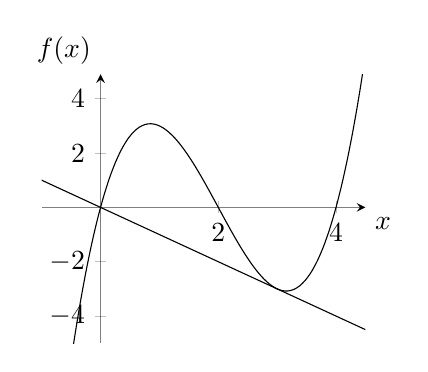
\begin{tikzpicture}
		\begin{axis}[scale=.6,draw opacity =.5,samples=100,smooth, 
		  axis x line=center, % no box around the plot, only x and y axis
		  axis y line=center, % the * suppresses the arrow tips
		  ylabel = {$f(x)$},
		  xlabel = {$x$},
		  xlabel style={below right},
		  ylabel style={above left},
		  xmin=-1,xmax=4,ymin=-5,ymax=4,
		  enlargelimits=upper] % extend the axes a bit to the right and top
		  \addplot[black,opacity=1]{x^3-6*x^2+8*x};
		  \addplot[black,opacity=1]{-x};
		\end{axis}
	    \end{tikzpicture}
	    \end{center}
	    \vspace{.5cm}
	    Primero calculemos la derivada de la recta y la curva, respectivamente
	    $$y'=-1,\qquad y_0'=3x^2-12x+8$$
	    Luego igualando estas ecuaciones obtenemos
	    $$y_1=3x^2-12x+8=-1\quad \Rightarrow \quad  x_1 = 3;\quad x_2=1.$$
	    Luego, para que la linea sea tangente a la curva, el punto debe estar en la curva $y_0=x^3-6x^2+8x$ como sigue,
	    \begin{itemize}
		\item Para $x_1=3$, se tiene $y(3)=-3=-x$ por lo que $y=-x$ es tangente a la curva en $(3,-3)$.\\
		\item Para $x_2=1$, se tiene $y(1)=1\neq -x$ por lo que $x_2$ no es tangente a la curva.\\
	    \end{itemize}
	    Esta linea tangente también corta la curva en $(0,0)$.\\\\

    %--------------------8.
    \item Dibujar la gráfica de la función cúbica $f(x)=x-x^3$ en el intervalo cerrado $-2\leq x\leq 2$. Hallar las constantes $m$ y $b$ de modo que la recta $y=mx+b$ sea tangente a la gráfica de $f$ en el punto $(-1,0)$. Una segunda recta que pasa por $(-1,0)$ es también tangente a la gráfica de $f$ en el punto $(a,c)$. Determinar las coordenadas $a$ y $c$.\\\\
	Respuesta.-\; 
	    \begin{center}
		\begin{tikzpicture}
		\begin{axis}[scale=.6,draw opacity =.5,samples=100,smooth, 
		  axis x line=center, % no box around the plot, only x and y axis
		  axis y line=center, % the * suppresses the arrow tips
		  ylabel = {$f(x)$},
		  xlabel = {$x$},
		  xlabel style={below right},
		  ylabel style={above left},
		  xmin=-2,xmax=2,ymin=-7,ymax=7,
		  enlargelimits=upper] % extend the axes a bit to the right and top
		  \addplot[black,opacity=1]{x-x^3};
		\end{axis}
	    \end{tikzpicture}
	    \end{center}
	    \vspace{.5cm}
	    Sea $f'(x)=1-3x^2$, entonce la tangente de la linea en el punto $(-1,0)$ será
	    $$f'(-1)=1-3(-1)^2 = -2 \quad \Rightarrow \quad m=-2.$$
	    de donde $b$ estará dado por,
	    $$y=mx+b\quad \Rightarrow \quad 0=-2(-1)+b \quad \Rightarrow \quad b=-2.$$
	    Por lo tanto 
	    $$y=-2x-2.$$
	    Después, supongamos otra linea tangente $y_1=m_1x+b_1$ a $f$ en el punto $(a,c)$ con pendiente 
	    $$f'(a)=1-3a^2=m_1$$
	    sabiendo que esta recta pasa por $(-1,0)$, entonces 
	    $$y_1(1)=0\quad \Rightarrow \quad (1-3a^2)(-1)+b_1=0\quad \Rightarrow \quad b_1=1-3a^2$$
	    Por lo que la recta $y_1$ es de la forma,
	    $$y_1=(1-3a^2)x+(1-3a^2).$$
	    Por último, dado que el punto $(a,c)$ está tanto en esta linea $y_1$ como en la curva $f$ tenemos
	    $$f(a)=c\quad \Rightarrow \quad a-a^3=c$$
	    $$\mbox{y}\qquad$$ 
	    $$y_1(a)=c\quad \Rightarrow \quad (1-3a^2)a+(1-3a^2)=c.$$
	    Igualando $c$ se tiene,
	    $$a-a^3=(1-3a^2)a+(1-3a^2) \quad \Rightarrow\quad 2a^3+3a^2-1=0 \quad \Rightarrow \quad 2a=\dfrac{1}{2}.$$
	    Ya que $a-a^3=c$ entonces $c=\dfrac{3}{8}.$ Así, el otro punto tangente está dado por $\left(\frac{1}{2},\frac{3}{8}\right).$\\\\

    %--------------------9.
    \item Una función $f$ está definida del modo siguiente:
    $$f(x)=\left\{\begin{array}{rcl}
	    \dfrac{1}{|x|}&\mbox{si}&|x|>c,\\\\
	    a+bx^2 &\mbox{si}&|x|\leq c.\\\\
    \end{array}\right.$$
    Hallar los valores de $a$ y $b$ (en función de $c$) tales que $f'(c)$ exista.\\\\
	Respuesta.-\; Sabemos que la derivada $f'(c)$ existe si y sólo si
	$$\lim_{h\to 0}\dfrac{f(c+h)-f(c)}{h}$$
	Existe. También sabemos que el límite existe si
	$$\lim_{h\to 0^+}\dfrac{f(c+h)-f(c)}{h} = \lim_{h\to 0^-}\dfrac{f(c+h)-f(c)}{h}.$$
	Por lo que si tomamos $c$ y nos acercamos a $ax+b$ desde la derecha, a $x^2$ desde la izquierda y tomando a $f(c)=c^2$, entonces 
	$$\begin{array}{rcl}
	    \lim\limits_{h\to 0^+} \dfrac{f(c+h)-f(c)}{h} &=& \lim\limits_{h\to 0^-} \dfrac{f(c+h)-f(c)}{h} \\\\
	    \lim\limits_{h\to 0^+} \dfrac{a(c+h)+b-c^2}{h} &=& \lim\limits_{h\to 0^-} \dfrac{(c+h)^2-c^2}{h} \\\\
	    \lim\limits_{h\to 0^+} \dfrac{ac+b-c^2}{h} + a &=& 2c.\\\\
	\end{array}$$
	Dado que $ac+b-c^2$ es una constante, entonces $\lim\limits_{h\to 0^+}\dfrac{ac+b-c^2}{h} = 0.$ Por lo que nos queda la ecuación 
	$$a=2c.$$
	Ahora dado que $\lim\limits_{h\to 0^+}\dfrac{ac+b-c^2}{h} = 0$, entonces
	$$ac+b-c^2=0 \quad \Rightarrow \quad b=-c^2.$$\\

    %--------------------10.
    \item Resolver el ejercicio 9 cuando $f$ es:
    $$f(x)=\left\{\begin{array}{lcl}
	    \dfrac{1}{|x|}&\mbox{si}&|x|>c,\\\\
	    a+bx^2 &\mbox{si}&|x|\leq c.\\
    \end{array}\right.$$\\
	Respuesta.-\; Supongamos que $c>0$ de lo contrario $f(x)=\dfrac{1}{|x|}$ para todo $x$. Entonces, existe la derivada para todo los valores de las constantes de $a$ y $b$. Luego sabemos que si una función tiene derivada en un punto $x$, entonces también es continua en $x$, por lo tanto la función $f$ es continua en $c$, así,\\
	$$\begin{array}{rcl}
	    \lim\limits_{x\to c^+}f(x)&=&\lim\limits_{x\to c^-}f(x)\\\\
	    \lim\limits_{x\to c^+}\dfrac{1}{|x|}&=&\lim\limits_{x\to c^-}a+bx^2\\\\
	    \dfrac{1}{c}&=&a+bc^2\\\\
			ac+bc^3&=&1\\\\
	\end{array}$$
	por otro lado,
	$$\begin{array}{rcl}
	    \lim\limits_{x\to 0^+}f(x)&=&\lim\limits_{x\to 0^-}f(x)\\\\
	    \lim\limits_{x\to 0^+}\dfrac{\frac{1}{|c+h|}-a+bc^2}{h}&=&\lim\limits_{x\to 0^-}\dfrac{a+b(c+h)^2-(a+bc^2)}{h}\\\\
	    \lim\limits_{x\to 0^+}\dfrac{\frac{1}{c+h}-a+bc^2}{h}\cdot \dfrac{c+h}{c+h}&=&\lim\limits_{x\to 0^-}\dfrac{2bch+bh^2}{h}\\\\
	    \lim\limits_{x\to 0^+}\dfrac{1-ac-bc^3-ah-bc^2h}{h(c+h)}&=&\lim\limits_{x\to 0^-}\dfrac{h(2bc+bh)}{h}\\\\
	    \lim\limits_{x\to 0^+}\dfrac{ac+bx^3-ac-bc^3-ah-bc^2h}{h}&=&\lim\limits_{x\to 0^-}2bc+bh\\\\
	    \lim\limits_{x\to 0^+}\dfrac{-h(a+bc^2)}{h(c+h)}&=&2bc+\lim\limits_{x\to 0^-}bh\\\\
	    \lim\limits_{x\to 0^+}-\dfrac{a+bc^2}{c+h}&=&2bc.\\\\
	    -\dfrac{a+bc^2}{c}&=&2bc.\\
	\end{array}$$
	Por último resolvemos las dos ecuaciones anteriores:
	$$\left\{\begin{array}{rcl}
		-\dfrac{a+bc^2}{c}&=&2bc\\\\
			   ac+bc^3&=&1\\
	\end{array}\right.
	\quad \Rightarrow \quad 
	\left\{\begin{array}{rcl}
		b &=& -\dfrac{1}{2c^3}\\\\
		a &=& -\dfrac{3}{2c}\\
	    \end{array}\right.$$\\\\

    %--------------------11.
    \item Resolver el ejercicio 9 cuando $f$ es:
    $$f(x)=\left\{\begin{array}{lcl}
	\sen x &\mbox{si}&x\leq c\\\\
	ax+b &\mbox{si}&x>c.\\
    \end{array}\right.$$\\\\
	Respuesta.-\; Sabemos que $f'(c)$ existe si y sólo si 
	$$\lim_{h\to 0}\dfrac{f(c+h)-f(c)}{h}$$
	Existe. También sabemos que el límite existe si y sólo si los dos límites unilaterales existen y son iguales, es decir
	$$\lim_{h\to 0^+}\dfrac{f(c+h)-f(c)}{h}=\lim_{h\to 0^-}\dfrac{f(c+h)-f(c)}{h}$$
	Por lo tanto usando la definición de $f$ tenemos,
	$$\begin{array}{rcl}
	    \lim\limits_{h\to 0^+} \dfrac{a(c+h)+b-\sen c}{h} &=& \lim\limits_{h\to 0^-} \dfrac{\sen (c+h)-\sen c}{h} \\\\
	    \lim\limits_{h\to 0^+} \left(\dfrac{ac + b-\sen c}{h}\right)+a &=& \lim\limits_{h\to 0^-} \dfrac{\sen c \cos h + \sen h \cos c - \sen c}{h}\\\\
	    \lim\limits_{h\to 0^+} \left(\dfrac{ac + b-\sen c}{h}\right)+a &=& \lim\limits_{h\to 0^-} \left[\dfrac{\sen c ( \cos h -1)}{h}\right] + \cos c \\\\
	\end{array}$$

	Al simplificar el lado derecho usamos el hecho de que $\lim\limits_{h\to 0}\dfrac{\sen h}{h}=1$. Además para que existe el límite por el lado izquierdo debemos tener $ac+b-\sen c = 0$ de lo contrario el límite divergirá como $h\to 0$. Ahora, para la expresión de la derecha, vemos que el límite tiende a $0$. Eso se puede ver ya que 
	$$\lim_{h\to 0^-}\dfrac{\sen c(\cos h - 1)}{h}=\sen c \lim_{h\to c^-}\dfrac{\cos h - 1}{h} = \sen c \lim_{h\to c^-}\dfrac{\cos(0+h)-\cos 0}{h}$$
	Pero este límite es la derivada de $\cos x$ en $x=0$. Luego ya que $(\cos x)'=-\sen x$ y $\sen 0 =0$ el termino tiende a $0$. Por lo tanto
	$$\lim\limits_{h\to 0^+} \left(\dfrac{ac + b-\sen c}{h}\right)+a = \lim\limits_{h\to 0^-} \left[\dfrac{\sen c ( \cos h -1)}{h}\right] + \cos c \quad \Rightarrow \quad a=\cos c.$$
	Así, dado que $ac+b-\sen c=0$ entonces 
	$$b=\sen c - c\cos c.$$\\

    %--------------------12.
    \item Si $f(x)=\dfrac{1-\sqrt{x}}{1+\sqrt{x}}$ para $x>0$, hallar fórmulas para $Df(x),\; D^2f(x)$ y $D^3f(x)$.\\\\
	Respuesta.- \; La fórmula para $Df(x)$ es:
	$$Df(x)=\dfrac{(1+\sqrt{x})\cdot \dfrac{-1}{2\sqrt{x}}- (1-\sqrt{x})\cdot \dfrac{1}{2\sqrt{x}}}{(1+\sqrt{x})^2} = \dfrac{\dfrac{1}{2}-\dfrac{1}{2}-\dfrac{1}{2\sqrt{x}}-\dfrac{1}{2\sqrt{x}}}{(1+\sqrt{x})^2}=\dfrac{-\dfrac{2}{2\sqrt{x}}}{(1+\sqrt{x})^2} =\dfrac{-1}{\sqrt{x}(1+\sqrt{x})^2}.$$

	Para $D^2f(x)$,

	$$D^2f(x)=\dfrac{\dfrac{1}{2\sqrt{x}}(1+\sqrt{x})^2+2\sqrt{x}(1+\sqrt{x})\dfrac{1}{2\sqrt{x}}}{x(1+\sqrt{x})^4} = \dfrac{1+3\sqrt{x}}{2(x+\sqrt{x})^3}.$$

	Por último para $D^3f(x)$,

	$$D^3f(x)=\dfrac{\dfrac{3}{2\sqrt{x}}\cdot 2(x+\sqrt{x})^3-6(1+3\sqrt{x})(x+\sqrt{x})^2\left(1+\dfrac{1}{2\sqrt{x}}\right)}{4(x+\sqrt{x})^6}=- \dfrac{3(1+4\sqrt{x}+5x)}{4\left[\sqrt{x}(x+\sqrt{x})^4\right]}.$$\\

    %--------------------13.
    \item Existe un polinomio $P(x)=ax^3+bx^2+cx+d$ tal que $P(0)=P(1)=-2,\; P'(0)=-1$ y $P''(0)=10.$Calcular $a,b,c,d.$\\\\
	Respuesta.-\; Primeramente calculamos la primera y segunda derivada de $P(x)$:
	$$P'(x)=ax^3+bx^2+cx+d,\qquad P''(x)=6ax+2b.$$
	De donde 
	$$P''(0)=6\cdot a\cdot 0+2b=10\quad \Rightarrow \quad b=5.$$
	$$\mbox{y}$$
	$$P'(0)=3\cdot a\cdot 0^2+2\cdot b \cdot 0 + c = -1 \quad \Rightarrow \quad c=-1.$$

	Luego calculamos $d$ y $a$ de la siguiente manera:
	$$P(0)=a\cdot 0^3+5\cdot 0^2-0+d=-2\quad \Rightarrow \quad d=-2.$$

	$$P(1)=a\cdot 1^3+5\cdot 1^2-1-2=-2\quad \Rightarrow \quad a=-4.$$

	Por lo tanto,
	$$a=-4,\quad b=5,\quad c=-1,\quad d=-2.$$\\

    %--------------------14.
    \item Dos funciones $f$ y $g$ admiten primera y segunda derivada en $0$ y satisfacen las relaciones 
	$$f(0)=\dfrac{2}{g(0)},\quad f'(0)=2g'(0)=4g(0),\quad g''(0)=5f''(0)=6f(0)=3.$$\\

	\begin{enumerate}[a)]

	    %---------- a)
	    \item Póngase $h(x)=\dfrac{f(x)}{g(x)}$, y calcular $h'(0).$\\\\
		Respuesta.-\; Usando la regla de derivada se tiene,
		$$h(x)=\dfrac{f(x)}{g(x)}\quad \Rightarrow \quad h'(x)=\dfrac{f'(x)-g(x)-f(x)g'(x)}{g^2(x)}.$$
		de donde sustituyendo obtenemos,
		$$\begin{array}{rcccl}
		    h'(0)&=&\dfrac{f'(0)g(0)-f(0)g'(0)}{g^2(0)}&=&\dfrac{4g^2(0)-f(0)g'(0)-\frac{2}{g(0)}2g(0)}{g^2(0)}\\\\
			 &=&\dfrac{4g^2(0)}{g^2(0)}-\dfrac{4}{g^2(0)} &=& 4-\dfrac{4}{\frac{4}{f^2(0)}}\\\\
			 &=& 4-\dfrac{4}{\frac{4}{\left(\frac{1}{2}\right)^2}}&=&\dfrac{15}{4}
		\end{array}$$
		\vspace{.7cm}

	    %---------- b)
	    \item Póngase $k(x)=f(x)g(x)\sen x$, y calcular $k'(0).$\\\\
		Respuesta.-\; Usando la propiedad del producto derivamos como sigue,\\
		$$k'(x)=f'(x)g'(x)\sen x + f(x)g'(x)\sen x + f(x)g(x)\cos x$$
		Luego evaluamos en $0$,
		$$k'(0)=f'(0)g'(0)\sen 0 + f(0)g'(0)\sen 0 + f(0)g(0)\cos 0 = f(0)g(0)=2.$$\\

	    %---------- c)
	    \item Calcular el límite de $\dfrac{g'(x)}{f'(x)}$ cuando $x\to 0$.\\\\
		Respuesta.-\; Sabemos que si $f$ y $g$ son diferenciables entonces son continuos, esto significa
		$$\lim_{x\to 0}f'(x)=f'(0)\quad \mbox{y}\quad \lim_{x\to 0}g'(x)=g'(0)$$
		Además $f'(0)\neq 0$ ya que $f'(0)=4g(0)$ y $g(0)=\dfrac{2}{f(0)}=\dfrac{2}{\frac{1}{2}}=4$, por lo tanto
		$$\lim_{x\to 0}\dfrac{g'(x)}{f'(x)}=\dfrac{\lim\limits_{x\to 0}g'(x)}{\lim\limits_{x\to 0}f'(x)}=\dfrac{g'(0)}{f'(0)}=\dfrac{g'(0)}{2g'(0)}=\dfrac{1}{2}.$$\\

	\end{enumerate}

    %--------------------15.
    \item Supóngase que existe la derivada $f'(a)$. Indicar cuáles de las desigualdades siguientes son ciertas y cuáles falsas. Expresar el fundamento de la decisión en cada caso.

	\begin{enumerate}[(a)]

	    %---------- (a)
	    \item $f'(a)=\lim\limits_{h\to a}\dfrac{f(h)-f(a)}{h-a}$.\\\\
		Respuesta.-\; Sea $j=h-a$ entonces
		$$\lim_{h\to a}\dfrac{f(h)-f(a)}{h-a}=\lim_{h\to a}\dfrac{f(a-a+h)-f(a)}{h-a}=\lim_{j\to 0}\dfrac{f(a+j)-f(a)}{j}=f'(a).$$
		Por lo que $f'(a)$ es verdadera.\\\\

	    %---------- (b)
	    \item $f'(a)=\lim\limits_{h\to 0}\dfrac{f(a)-f(a+h)}{h}$.\\\\
		Respuesta.-\; Sea $j=-h$, entonces
		$$\lim_{h\to 0}\dfrac{f(a)-f(a-h)}{h}=\lim_{h\to a}\dfrac{f(a)-f(a+j)}{-j}=\lim_{t\to 0}\dfrac{f(a+j)-f(a)}{j}.$$\\
		Por lo tanto $f'(a)$ es verdadera.\\\\

	    %---------- (c)
	    \item $f'(a)=\lim\limits_{t\to 0}\dfrac{f(a+2t)-f(a)}{t}$.\\\\
		Respuesta.-\; Sea $j=2t$, entonces
		$$\lim_{t\to 0}\dfrac{f(a+2t)-f(a)}{t}=\lim_{t\to 0}=2\cdot\dfrac{f(a+2t)-f(a)}{2t}=2\cdot \lim_{t\to 0}\dfrac{f(a+j)-f(a)}{j}=2f'(a)\neq f'(a).$$\\
		Por lo tanto $f'(a)$ es falsa.\\\\

	    %---------- (d)
	    \item $f'(a)=\lim\limits_{t\to 0}\dfrac{f(a+2t)-f(a+t)}{2t}$.\\\\
		Respuesta.-\; Sea $j=2t$, entonces
		$$\begin{array}{rcl}
		    \lim\limits_{t\to 0}\dfrac{f(a+2t)-f(a+t)}{2t}&=&\lim\limits_{t\to 0}\dfrac{f(a+2t)-f(a+t)+f(a)-f(a)}{2t}\\\\
						  &=&\lim\limits_{t\to 0}\dfrac{f(a+2t)-f(a)}{2t}-\lim\limits_{t\to 0}\dfrac{f(a+t)-f(a)}{2t}\\\\
						  &=&\lim\limits_{t\to 0}\dfrac{f(a+j)-f(a)}{j}-\dfrac{1}{2}\cdot \lim\limits_{t\to 0}\dfrac{f(a+t)-f(a)}{t}\\\\
						  &=&f'(a)-\dfrac{1}{2}f'(a)\\\\
						  &=&\dfrac{1}{2}f'(a)\neq f'(a).\\\\
		\end{array}$$
		Por lo tanto $f'(a)$ es falsa.\\\\

	\end{enumerate}

    %--------------------16.
    \item Supóngase que en lugar de la definición usual de derivada $Df(x)$ se define una nueva clase de derivada $D^*f(x)$ por fórmula:
	$$D^*f(x)=\lim_{h\to 0}\dfrac{f^2(x+h)-f^2(x)}{h},$$
	donde $f^2(x)$ significa $[f(x)]^2.$\\

	\begin{enumerate}[(a)]

	    %---------- (a)
	    \item Hallar fórmulas para calcular la derivada $D^*$ de una suma, diferencia, producto y cociente.\\\\
		Respuesta.-\; Sea $f$ y $g$. Para la suma se tiene,
		$$\begin{array}{rcl}
		    D^*\left[f(x)+g(x)\right]&=&\lim\limits_{h\to 0}\dfrac{\left[f(x+h)+g(x+h)\right]^2-\left[f(x)+g(x)\right]^2}{h}\\\\
					     &=&\lim\limits_{h\to 0}\dfrac{f^2(x+h)+2f(x+h)(x+h)+g^2(x+h)-f^2(x)-2f(x)g(x)-g^2(x)}{h}\\\\
					     &=&\lim\limits_{h\to 0}\left[\dfrac{f^2(x+h)-f^2(x)}{h}\right]+2\lim\limits_{h\to 0}\left[\dfrac{f(x+h)g(x+h)-f(x)g(x)}{h}\right]\\\\
					     &+&\lim\limits_{h\to 0}\left[\dfrac{g^2(x+h)-g^2(x)}{h}\right]\\\\
					     &=&D^*f(x)+d^*g(x)+2\lim\limits_{h\to 0}\left[\dfrac{f(x+h)g(x+h)-f(x)g(x)}{h}\right].\\\\
		\end{array}$$
		Luego multiplicamos el límite anterior por $\dfrac{f(x+h)g(x+h)+f(x)g(x)}{f(x+h)g(x+h)+f(x)g(x)}$, de donde
		$$\begin{array}{rcl}
		    &=&D^*f(x)+f^*g(x)+2\lim\limits_{h\to 0}\left[\dfrac{f(x+h)g(x+h)-f(x)g(x)}{h}\cdot \dfrac{f(x+h)g(x+h)+f(x)g(x)}{f(x+h)g(x+h)+f(x)g(x)}\right]\\\\
		    &=&D^*f(x)+D^*g(x)+2\lim\limits_{h\to 0}\left[\dfrac{f^2(x+h)g^2(x+h)-f^2(x)g^2(x)}{h\left(f(x+h)g(x+h)+f(x)g(x)\right)}\right]\\\\
		    &=&D^*f(x)+D^*g(x)+\dfrac{1}{f(x)g(x)}\lim\limits_{h\to 0}\dfrac{\left[f(x+h)g(x+h)\right]-\left[f(x)g(x)\right]^2}{h}.\\\\
		\end{array}$$
		Ahora, para el límite restante, usamos la regla del producto para la derivada en esta definición alternativa, que derivamos a continuación. (Este último límite es $D^* (f(x)g(x))$. Luego derivamos que $D^* (f(x)g(x)) = g^2 D^*f + f^2 D^* g)$. Por lo tanto,
		$$\begin{array}{rcl}
		    D^*\left[f(x)+g(x)\right] &=&D^*f(x)+D^*g(x)+\dfrac{1}{f(x)g(x)}\lim\limits_{h\to 0}\dfrac{\left[f(x+h)g(x+h)\right]-\left[f(x)g(x)\right]^2}{h}.\\\\
					      &=&D^*f(x)+D^*g(x)+\dfrac{1}{f(x)g(x)}\left[g^2(x)D^*f(x)+f^2(x)D^*g(x)\right]\\\\
					      &=&D^*f(x)+D^*g(x)+\dfrac{g(x)}{f(x)}D^*f(x)+\dfrac{f(x)}{g(x)}D^*g(x)\\\\
					      &=&\left(1+\dfrac{g(x)}{f(x)}\right)D^*f(x)+\left(1+\dfrac{f(x)}{g(x)}\right)D^*g(x)\\\\
		\end{array}$$

		Para la diferencia se sigue similar a la suma,

		$$D^*\left[f(x)-g(x)\right]=\left(1-\dfrac{g(x)}{f(x)}\right)D^*f(x)+\left(1-\dfrac{f(x)}{g(x)}\right)D^*g(x)$$

		Para el producto tenemos,

		$$\begin{array}{rcl}
		    D^*\left[f(x)g(x)\right] &=&\lim\limits_{h\to 0}\dfrac{\left[f(x+h)g(x+h)\right]^2-\left[f(x)g(x)\right]^2}{h}\\\\ 
					     &=&\lim\limits_{h\to 0}\dfrac{f^2(x+h)g^2(x+h)-f^2(x)g^2(x)}{h}\\\\
					     &=&\lim\limits_{h\to 0}\dfrac{f^2(x+h)g^2(x+h)-f^2(x)g^2(x)+f^2(x+h)g^2(x)-f^2(x+h)g^2(x)}{h}\\\\
					     &=&\lim\limits_{h\to 0}\left[g^2(x)\dfrac{f^2(x+h)-f^2(x)}{h}\right]+\lim\limits_{h\to 0}\left[f^2(x+h)\dfrac{g^2(x+h)-g^2(x)}{h}\right]\\\\
					     &=&g^2(x)D^*f+f^2(x)D^*g.\\\\

		\end{array}$$

		Por último para el cociente tenemos,

		$$\begin{array}{rcl}
		    D^*\left[\dfrac{f(x)}{g(x)}\right]&=&\lim\limits_{h\to 0}\dfrac{\frac{f^2(x+h)}{g^2(x+h)}-\frac{f^2(x)}{g^2(x)}}{h}\\\\
						      &=&\lim\limits_{h\to 0}\left[\dfrac{g^2(x)f^2(x+h)-f^2(x)g^2(x+h)}{h\cdot g^2(x+h)g^2(x)}\right]\\\\
						      &=&\dfrac{1}{g^4(x)}\lim\limits_{h\to 0}\left[\dfrac{g^2(x)f^2(x+h)-f^2(x)g^2(x+h)+g^2(x)f^2(x)-g^2(x)f^2(x)}{h}\right]\\\\
						      &=&\dfrac{1}{g^4(x)}\lim\limits_{h\to 0}\left[g^2(x)\dfrac{f^2(x+h)-f^2(x)}{h}-f^2(x)\dfrac{g^2(x+h)-g^2(x)}{h}\right]\\\\
						      &=&\dfrac{g^2D^*f-f^2D^*g}{g^4}\\\\
		\end{array}$$



	    %---------- (b)
	    \item Expresar $D^*f(x)$ en función de $Df(x)$.\\\\
		Respuesta.-\; Usaremos la idea de $\lim_{h \to 0} f(x+h) = f(x)$, y que $f(x)$ es una constante en $h$, por lo que podemos sacar el límite. 
		$$D^*f(x)=\lim_{h\to 0}\dfrac{f^2(x+h)-f^28x)}{h}=\lim_{h\to 0}\dfrac{\left[f(x+h)+f(x)\right]\left[f(x+h)-f(x)\right]}{h}=2f(x)\cdot Df(x).$$\\


	    %---------- (c)
	    \item ¿Para qué funciones es $D^*f=Df$?.\\\\
		Respuesta.-\; Para encontrar la función $f$ tal que $Df=D^*f$ igualamos las dos expresiones y resolvemos $f$ usando $D^*f=2D f$, como sigue
		$$Df=D^*f\quad \Rightarrow \quad Df=2f(x)Df\quad \Rightarrow \quad Df=0\; \mbox{o}\; 2f(x)=1.$$
		En cualquier caso tenemos $f(x)=c$ para alguna constante $c$.\\\\

	\end{enumerate}

\end{enumerate}


\section{Regla de la cadena para la derivación de funciones compuestas}

\begin{teo}[Regla de la cadena]
    Sea $f$ la función compuesta de dos funciones $u$ y $v$, expresado por $f=u\circ v.$ Suponga que ambas derivadas $v'(x)$ y $u'(y)$ existen, donde $y=v(x)$, entonces la derivada $f'(x)$ también existe y es dado por la fórmula 
    $$f'(x)=u'(y)\cdot v'(x)\quad \mbox{o}\quad f'(x)=u'[v(x)]\cdot v'(x)\quad \mbox{o}\quad (u\circ v)'=(u'\circ v)\cdot v'\quad \mbox{o}\quad u(v)'=u'(v)\circ v'.$$
    Dicho de otro modo, para calcular la derivada de $u\circ v$ respecto a $x$ se calcula primero la derivada de $u$ en el punto $y$ donde $y=v(x)$, y se multiplica ésta por $v'(x)$.\\\\
	Demostración.-\;  Se trata aquí de demostrar $f'(x)=u'(v)\cdot v'(x)$. Se supone que $v$ tiene derivada en $x$ y $u$ tiene derivada en $v(x)$ y se trata de demostrar que $f$ tiene derivada en $x$ dada por el producto $u'\left[v(x)\right]\cdot v'(x)$. El cociente de diferencia para $f$ es:
	$$\dfrac{f(x+h)-f(x)}{h}=\dfrac{u\left[v(x+h)\right]-y\left[v(x)\right]}{h}$$
	Ahora es conveniente introducir la siguiente notación: Sean $y=v(x)$ y sea $k=v(x+h)-v(x)$. Es importante poner de manifiesto que $k$ depende de $h$. Entonces se tiene $v(x+h)=y+k$, por lo que el cociente de diferencias de $f$ se transforma en:
	$$\dfrac{f(x+h)-f(x)}{h}=\dfrac{u(y+k)-u(y)}{h}$$
	El segundo miembro sería el cociente de diferencias cuyo límite define $u'(y)$, si en el denominador en vez de $h$ apareciera $k$. Si $k\neq 0$ se completa fácilmente la demostración multiplicando el numerador y el denominador por $k$ toma la forma:
	$$\dfrac{u(y+k)-u(y)}{k}\cdot \dfrac{k}{h}=\dfrac{u(y+k)-u(y)}{k}\cdot \dfrac{v(x+h)-v(x)}{h}.$$
	Cuando $h\to 0$ el último cociente del segundo miembro tiende a $v'(x)$. Puesto que $k=v(x+h)-v(x)$ y $v$ es continua en $x$, al tender $h\to 0$ también $k\to 0$; por tanto, el primer cociente del segundo miembro tiende a $u'(y)$ cuando $h\to 0$.\\
	Aunque el razonamiento precedente parece el camino más natural para la demostración, sin embargo no es completamente general. Como $k=v(x+h)-v(x)$, puede ocurrir que $k=0$ para infinitos valores de $h$ cuando $h\to 0$, en cuyo caso pasar a $\dfrac{u(y+k)-u(y)}{k}\cdot \dfrac{k}{h}=\dfrac{u(y+k)-u(y)}{k}\cdot \dfrac{v(x+h)-v(x)}{h}$ no es válido. Para soslayar esta dificultad es necesario modificar ligeramente la demostración.\\
	Volviendo a la ecuación $\dfrac{f(x+h)-f(x)}{h}=\dfrac{u(y+k)-u(y)}{h}$ se expresa el cociente del segundo miembro de manera que no aparezca $k$ en el denominador, para lo cual se introduce la diferencia entre la derivada $u'(y)$ y el cociente de diferencias cuyo límite es $u'(y)$. Es decir, se define una nueva función $g$ como sigue:
	$$g(t)=\dfrac{u(y+t)}{t}-u'(y)\, \mbox{si}\; t\neq 0.$$
	Esta ecuación define $g(t)$ sólo si $t\neq 0$. Multiplicando por $t$ y transponiendo términos, se puede escribir en la forma:
	$$u(y+t)-u(y)=t[g(t)+u'(y)].$$
	Aunque esta última forma se había deducido en la hipótesis de ser $t\neq 0$, es válida también para $t=0$ mientras se asigne algún valor definido a $g(0)$. El valor que se asigne a $g(0)$ no tiene importancia para esta demostración, pero ya que $g(t)\to 0$ cuando $t\to 0$ parece natural definir $g(0)$ igual a $0$. Si ahora se sustituye $t$ por $k$, donde $k=v(x+h)-v(x)$ y se sustituye el segundo miembro de $u(y+t)-u(y)=t[g(t)+u'(y)]$ en $\dfrac{f(x+h)-f(x)}{h}=\dfrac{u(y+k)-u(y)}{h}$ se obtiene:
	$$\dfrac{f(x+h)-f(x)}{k}=\dfrac{k}{h}[g(k)+u'(y)]$$
	fórmula que es válida aun cuando $k=0$. Si $h\to 0$ el cociente $k/h\to v'(x)$ y $g(k)\to 0$; por lo tanto el segundo miembro tiende al límite $u'(y)\cdot v'(x).$ Queda pues completada la demostración de la regla de la cadena.\\\\
\end{teo}

\section{Aplicaciones de la regla de cadena. Coeficientes de variación ligados y derivación implícita}

Introducimos los símbolos $$y=v(x)\qquad \mbox{y}\qquad z=u(y).$$

Y designando con $dy/dx$ la derivada $v'(x)$ y con $dz/dy$ la de $u(y)$, la formación de la función compuesta queda indicada por:
$$z=u(y)=u[v(x)]=f(x),$$
siguiente lo notación de Leibniz, $dz/dx$ designa la derivada $f'(x)$, la regla de la cadena tal como estaba expresada se presenta ahora en la forma:
$$\dfrac{dz}{dx}=\dfrac{dz}{dy}\cdot \dfrac{dy}{dx}$$

Si $y=v(x)$ y $z=f(x)$, entonces $z=y^n$, $dz/dx=f'(x)$ y la regla de la cadena da:
$$\dfrac{dz}{dx}=\dfrac{dz}{dy}\cdot \dfrac{dy}{dx}=ny^{n-1}v'(x)=n[v(x)]^{n-1}v'(x).$$\\

\begin{ejem}
    Si $f(x)=[v(x)]^n$ donde $n$ es un entero positivo, calcular $f'(x)$ en función de $v(x)$ y $v'8x)$. \\\\
	Respuesta.-\; La solución $f$ es una composición, $f(x)=u[v(x)]$, donde $y(x)=x^n$. Puesto que $u'(x)=nx^{n-1}$, se tiene $u'[v(x)]$ $u'[v(x)]=n[v(x)]^{n-1}v'(x).$ Y la regla de la cadena da:
	$$f'(x)=n[v(x)]^{n-1}v'(x).$$
	Si se omite la referencia a $x$ y se escribe como una igualdad entre funciones, se obtiene la importante fórmula:
	$$(v^n)'=nv^{n-1}v'$$
	que indica cómo se deriva la potencia n-ésima de $v$ cuando $v'$ existe. La fórmula es también válida para las potencias racionales si $v^n$ y $v^{n-1}$ están definidas.\\\\
\end{ejem}


\section{Ejercicios}
En los ejercicios del 1 al 14, determinar la derivada $f'(x)$. En cada caso se sobrentiende que $x$ toma sólo los valores para los que $f(x)$ tiene sentido.

\begin{enumerate}[\bfseries 1.]

    %--------------------1.
    \item $f(x)\cos 2x-2\sen x$.\\\\
	Respuesta.-\; Usando las reglas de derivación tenemos,
	$$f'(x)=(-\sen 2x )2-\left(0\cdot \sen x + 2\cos x\right) = -2\sen 2x-2\cos x.$$\\

    %--------------------2.
    \item $f(x)=\sqrt{1+x^2}$.\\\\
	Respuesta.-\; Usando las reglas de derivación tenemos,
	$$f'(x)=\dfrac{1}{2}(1+x^2)^{-\frac{1}{2}}\cdot 2x = \dfrac{x}{\sqrt{1+x^2}}.$$

    %--------------------3.
    \item $f(x)=(2-x^2)\cos x^2+2x\sen x^3.$\\\\
	Respuesta.-\; Usando las reglas de derivación tenemos,
	$$\begin{array}{rcl}
	    f'(x)&=&-2x\cos x^2+(2-x^2)(-2x\sen x^2)+2\sen x^3 \cdot 2\sen x^3+2x\cdot 3x^3\cdot \cos x^3\\
		 &=&(2x^3-4x)\sen x^2 - 2x \cos x^2 + 2\sen x^2 + 6x^3\cos x^3.\\\\
	\end{array}$$

    %--------------------4.
    \item $f(x)=\sen (\cos^2 x)\cdot \cos (\sen^2 x)$.\\\\
	Respuesta.-\; Usando las reglas de derivación tenemos,
	$$\begin{array}{rcl}
	    f'(x)&=&\cos\left(\cos^2 x\right)\left(-2\cos x \sen x\right)\cos\left(\sen^2 x\right)+\sen\left(\cos^2 x\right)\left[-\sen\left(\sen^2 x\right)\right]2\sen x \cos x\\
		 &=&\left(-2\sen x \cos x\right)\left[\cos\left(\cos^2 x\right)\cos\left(\sen^2 x\right)+\sen \left(\cos^2 x\right)\sen \left(\sen^2 x\right)\right]\\
		 &=&-\sen(2x)\left[\cos \left(\cos^2 x - \sen^2 x\right)\right]\\
		 &=&-\sen(2x)\cos\left(\cos 2 x\right).\\\\
	\end{array}$$


    %--------------------5.
    \item $f(x)=\sen^n x \cdot \cos nx$.\\\\
	Respuesta.- \; Por el hecho de que $(v^n)'=nv^{n-1}v'$ tenemos,
	$$\begin{array}{rcl}
	    f'(x)&=&n\left(\sen^{n-1}x\right)\cos x \cos nx + \sen^n x (-\sen nx)n\\
		 &=&\left(n\sen^{n-1}x\right)\left[\cos x \cos nx - \sen x \sen nx\right]\\
	 \end{array}$$
	 Luego por la identidad $\cos(x+y) = \cos x \cos y - \sen x \sen y$ concluimos que,
	 $$f'(x)=\left(n\sen^{n-1}x\right)\cos\left[(n+1)x\right].$$\\


    %--------------------6.
    \item $f(x)=\sen [\sen(\sen x)]$.\\\\
	Respuesta.-\; Usando las reglas de derivación tenemos,
	$$f'(x)=\cos\left[\sen(\sen x)\right]\cdot \cos(\sen x)\cdot \cos x.$$\\

    %--------------------7.
    \item $f(x)=\dfrac{\sen^2 x}{\sen x^2}$.\\\\
	Respuesta.- \; Usando las reglas de derivación tenemos,
	$$\begin{array}{rcl}
	    f'(x)&=&\dfrac{(2\sen x \cos x)\left[\sen\left(x^2\right)\right]-\left(\sen^2 x\right)\left[2x\cos \left(x^2\right)\right]}{\sen^2\left(x^2\right)}\\\\
		 &=&\dfrac{2\sen x\left[\cos x \sen \left(x^2\right)-x\sen x\cos \left(x^2\right)\right]}{\sen^2\left(x^2\right)}.\\\\
	\end{array}$$
	\vspace{.7cm}

    %--------------------8.
    \item $f(x)=\tan\dfrac{x}{2}-\cot\dfrac{x}{2}$.\\\\
	Respuesta.-\; Sabemos que $(\tan x)'=\sec^2 x$ y $(\cot x)'=csc^2 x$ por lo tanto,
	$$\begin{array}{rcl}
	    f'(x)&=&\dfrac{1}{2}\sec^2\left(\dfrac{x}{2}\right)+\dfrac{1}{2}\csc^2\left(\dfrac{x}{2}\right)\\\\
		 &=&\dfrac{1}{2}\left[\dfrac{1}{\cos^2\left(\dfrac{x}{2}\right)}+\dfrac{1}{\sen^2\left(\dfrac{x}{2}\right)}\right]\\\\
		 &=&\dfrac{1}{2}\left[\dfrac{\sen^2\left(\dfrac{x}{2}\right)+\cos^2\left(\dfrac{x}{2}\right)}{\sen^2\left(\dfrac{x}{2}\right)\cdot \cos^2\left(\dfrac{x}{2}\right)}\right]\\\\
		 &=&\dfrac{1}{2\left[\sen \left(\dfrac{x}{2}\right)\cos \left(\dfrac{x}{2}\right)\right]\left[\sen \left(\dfrac{x}{2}\right)\cos \left(\dfrac{x}{2}\right)\right]}\\\\
	\end{array}$$
	Luego ya que $\sen(2x)=2\sen x \cos x$, es decir 
	$$\sen x = \sen\left(\dfrac{2x}{2}\right)=2\sen \left(\dfrac{x}{2}\right)\cos \left(\dfrac{x}{2}\right)\quad \Rightarrow \quad \sen\left(\dfrac{x}{2}\right)\cos \left(\dfrac{x}{2}\right)=\dfrac{1}{2}\sen x.$$
	Se tiene,
	$$\dfrac{1}{2\cdot \dfrac{1}{2}\sen x\cdot \dfrac{1}{2}\sen x}=\dfrac{2}{\sen^2 x}.$$\\


    %--------------------9.
    \item $f(x)=\sec^2 x + csx^2 x$.\\\\
	Respuesta.-\; Simplificando la expresión dada, tenemos
	$$f(x)=\sec^2 x + \csc^2 x = \dfrac{1}{\cos^2x}+\dfrac{1}{\sen^2 x}=\dfrac{\sen^2 x + \cos^2 x}{\cos^2 x \sen^2 x}=\dfrac{1}{\dfrac{1}{4}\cdot \sen^2(2x)}=\dfrac{4}{\sen^2(2x)}$$
	Por lo tanto la derivada de $f$ estará dada por,
	$$f'(x)=\dfrac{-4[\cos(2x)][\sen(2x)]2}{\sen^4(2x)}=-\dfrac{16\cos(2x)}{\sen^3(2x)}.$$\\

    %--------------------10.
    \item $f(x)=x\sqrt{1+x^2}$.\\\\
	Respuesta.- \; Usando las reglas de derivación tenemos,
	$$f'(x)=\sqrt{1+x^2}+\dfrac{1}{2}\left(1+x^2\right)^{-\frac{1}{2}}\cdot2x = \sqrt{1+x^2}+\dfrac{x}{\sqrt{1+x^2}}=\dfrac{1+2x^2}{\sqrt{1+x^2}}.$$\\

    %--------------------11.
    \item $f(x)=\dfrac{x}{\sqrt{4-x^2}}$.\\\\
	Respuesta.- Usando las reglas de derivación tenemos,
	$$f'(x)=\dfrac{\sqrt{-x^2}-x\dfrac{1}{2}\left(4-x^2\right)^{-\frac{1}{2}}(-2x)}{\left(\sqrt{4-x^2}\right)^2}=\dfrac{4-x^2+x^2}{\left(4-x^2\right)^{\frac{3}{2}}}=\dfrac{4}{\left(4-x^2\right)^{\frac{3}{2}}}.$$\\

    %--------------------12.
    \item $f(x)=\left(\dfrac{1+x^3}{1-x^3}\right)^{1/3}$.\\\\
	Respuesta.- Usando las reglas de derivación tenemos,
	$$\begin{array}{rcl}
	    f'(x)&=&\dfrac{1}{3}\left(\dfrac{1+x^3}{1-x^3}\right)^{-\frac{2}{3}}\left[\dfrac{3x^2\left(1-x^3\right)-\left(1+x^3\right)\left(-3x^2\right)}{\left(1-x^3\right)^2}\right]\\\\
		 &=&\dfrac{1}{3}\left(\dfrac{1+x^3}{1-x^3}\right)^{-\frac{2}{3}}\cdot \dfrac{6x^2}{\left(1-x^3\right)^2}\\\\
		 &=&\dfrac{2x^2}{1-x^3}\cdot \dfrac{1}{1-x^3}\cdot \left(\dfrac{1+x^3}{1-x^3}\right)^{-\frac{2}{3}}\\\\
		 &=&\dfrac{2x^2\left(1-x^3\right)}{\left(1-x^3\right)\left(1+x^3\right)}\cdot \dfrac{1}{1-x^3}\cdot \left(\dfrac{1+x^3}{1-x^3}\right)^{-\frac{2}{3}}\\\\
		 &=&\dfrac{2x^2}{1-x^6}\cdot \dfrac{1+x^3}{1-x^3}\cdot \left(\dfrac{1+x^3}{1-x^3}\right)^{-\frac{2}{3}}\\\\
		 &=&\dfrac{2x^2}{1-x^6}\cdot \left(\dfrac{1+x^3}{1-x^3}\right)^{\frac{1}{3}}\\\\
	\end{array}$$
	\vspace{.7cm}

    %--------------------13.
    \item $f(x)=\dfrac{1}{\sqrt{1+x^2}\left(x+\sqrt{1+x^2}\right)}$.\\\\
	Respuesta.- \; Primeramente simplifiquemos la expresión dada,
	$$\begin{array}{rcl}
	    f(x)&=&\dfrac{1}{\sqrt{1+x^2}\left(\sqrt{1+x^2}+x\right)}\\\\
		&=&\dfrac{\sqrt{1+x^2}-x}{\sqrt{1+x^2}\left(\sqrt{1-x^2}-x\right)\left(\sqrt{1+x^2}-x\right)}\\\\
		&=&\dfrac{\sqrt{1+x^2}-x}{\sqrt{1+x^2}\left(1+x^2-x^2\right)}\\\\
		&=&1-\dfrac{x}{\sqrt{1+x^2}}.\\\\
	\end{array}$$
	Ahora, derivemos $f$ de la siguiente manera,
	$$f'(x)=-\left[\dfrac{\sqrt{1+x^2}-\dfrac{1}{2}\dfrac{x}{\sqrt{1+x^2}}2x}{1+x^2}\right]=-\dfrac{\sqrt{1+x^2}-\dfrac{x^2}{\sqrt{1+x^2}}}{1+x^2}=\dfrac{1}{\left(1+x^2\right)^{\frac{3}{2}}}.$$\\

    %--------------------14.
    \item $f(x)=\sqrt{x+\sqrt{x+\sqrt{x}}}$.\\\\
	Respuesta.-\; Sea $g(x)=\sqrt{x+\sqrt{x}}$, entonces
	$$g'(x)=\dfrac{1}{2\sqrt{x\sqrt{x}}}\left(1+\dfrac{1}{2\sqrt{x}}\right)=\dfrac{1}{2\sqrt{x+\sqrt{x}}}+\dfrac{1}{4\sqrt{x}\sqrt{x+\sqrt{x}}}=\dfrac{1}{2g(x)}+\dfrac{1}{3\sqrt{x}g(x)}.$$
	Luego usando $g(x)$ en la ecuación del enunciado tenemos,
	$$\begin{array}{rcl}
	    g'(x)&=&\sqrt{x+g(x)}\\\\
		 &=&\dfrac{1}{2\sqrt{x+g(x)}}\left(1+g'(x)\right)\\\\
		 &=&\dfrac{1}{2\sqrt{x+g(x)}}\left(1+\dfrac{1}{2g(x)}+\dfrac{1}{4\sqrt{x}g(x)}\right)\\\\
		 &=&\dfrac{4\sqrt{x}g(x)+2\sqrt{x}+1}{8\sqrt{x}g(x)\sqrt{x+g(x)}}.\\\\
	\end{array}$$
	\vspace{.7cm}

    %--------------------15.
    \item Calcular $f'(x)$ si $f(x)=(1+x)(2+x^2)^{1/2}(3+x^3)^{1/3}, \; x^3\neq -3.$\\\\
	Respuesta.-\; Aplicando las reglas de derivación tenemos,
	$$\begin{array}{rcl}
	    f'(x)&=&\left(2+x^2\right)^{1/2}\left(3+x^3\right)^{1/3}+(1+x)\left[\dfrac{1}{2}\left(2+x^2\right)^{-1/2}\left(3+x^3\right)^{1/3}+\left(2+x^2\right)^{1/2}\dfrac{1}{3}\left(\right)^{-2/3}3x^2\right]\\\\
		 &=&\left(\right)^{1/2}\left(3+x^3\right)^{1/3}+(1+x)\left(3+x^3\right)^{1/3}\dfrac{x}{\left(2+x^2\right)^{1/2}}+(1+x)\left(2+x^2\right)^{1/2}\dfrac{x^2}{\left(3+x^3\right)^{2/3}}\\\\
		 &=&\dfrac{3x^5+2x^4+4x^3+8x^2+3x+6}{\left(2+x^2\right)^{1/2}\left(3+x^3\right)^{2/3}}.\\\\
	\end{array}$$
	\vspace{.7cm}

    %--------------------16.
    \item Sean $f(x)=\dfrac{1}{1+1/x}$ si $x\neq 0\;$ y $\;g(x)=\dfrac{1}{1+1/f(x)}.$ Calcular $f'(x)$ y $g'(x)$.\\\\
	Respuesta.-\; Sea $f(x)=\dfrac{1}{1+1/x}=\dfrac{x}{x+1}$, entonces aplicando las reglas de derivación tenemos,
	$$f'(x)=\dfrac{(x+1)-x}{(x+1)^2}=\dfrac{1}{(x+1)^2}.$$

	Luego sea $g(x)=\dfrac{1}{1+1/f(x)}=\dfrac{1}{1+\dfrac{1}{\frac{1}{1+1/x}}}=\dfrac{1}{2+x^{-1}}$ entonces la derivada de $g$ estará dada por,
	$$g'(x)=\dfrac{x^{-2}}{\left(2+x^{-1}\right)^2}=\dfrac{1}{x^2\left(4+4x^{-1}+x^{-2}\right)^2}=\dfrac{1}{(2x+1)^2}.$$\\

    %--------------------17.
    \item La siguiente tabla de valores se calculó sus derivadas respectivas para  $f'$ y $g'$. Construir la correspondiente tabla para las dos funciones compuestas $h$ y $k$ dadas por $h(x)=f[g(x)]$, $k(x)=g[f(x)]$.\\

	$$\begin{array}{c|c|c|c|c}
	    x&f(x)&f'(x)&g(x)&g'(x)\\\\
	    \hline\\
	     0&1&5&2&-5\\
	     1&3&-2&0&1\\
	     2&0&2&3&1\\
	     3&2&4&1&-6\\
	\end{array}$$
	\vspace{.7cm}

	Respuesta.-\;

	$$h(x)=\left\{\begin{array}{rclclcl}
	    h(0)&=&f(g(0))&=&f(2)&=&0\\
	    h(1)&=&f(g(1))&=&f(0)&=&1\\
	    h(2)&=&f(g(2))&=&f(3)&=&2\\
	    h(3)&=&f(g(3))&=&f(1)&=&3\\
	\end{array}\right. 
	\qquad 
	k(x)=\left\{\begin{array}{rclclcl}
	    k(0)&=&g(f(0))&=&g(1)&=&0\\
	    k(1)&=&g(f(1))&=&g(3)&=&1\\
	    k(2)&=&g(f(2))&=&g(0)&=&2\\
	    k(3)&=&g(f(3))&=&g(2)&=&3\\
	\end{array}\right.$$

	$$h'(x)=f'(g(x))g'(x)=\left\{\begin{array}{rclclcr}
	    h'(0)&=&f'(g(0))g'(0)&=&f'(2)(-5)&=&-10\\
	    h'(1)&=&f'(g(1))g'(1)&=&f'(0)(1)&=&5\\
	    h'(2)&=&f'(g(2))g'(2)&=&f'(3)(1)&=&4\\
	    h'(3)&=&f'(g(3))g'(3)&=&f'(1)(-6)&=&12\\
	\end{array}\right.$$

	$$k(x)=g'(f(x))f'(x)=\left\{\begin{array}{rclclcr}
	    k'(0)&=&g'(f(0))f'(0)&=&g'(1)(5)&=&5\\
	    k'(1)&=&g'(f(1))f'(1)&=&g'(3)(-2)&=&12\\
	    k'(2)&=&g'(f(2))f'(2)&=&g'(0)(2)&=&-10\\
	    k'(3)&=&g'(f(3))f'(3)&=&g'(2)(4)&=&4\\
	\end{array}\right.$$
	\vspace{.7cm}

    %--------------------18.
    \item Una función $f$ y sus dos primeras derivadas se han tabulado como se indica. Poner $g(x)=xf\left(x^2\right)$ y construir una tabla de $g$ y sus dos primeras derivadas para $x=0,1,2.$
	$$\begin{array}{c|c|c|c}
	    x&f(x)&f'(x)&f''(x)\\\\
	    \hline\\
	     0&0&1&2\\
	     1&1&1&1\\
	     2&3&2&1\\
	     3&6&3&0\\
	\end{array}$$
	\vspace{.5cm}

	Respuesta.-\; Sean $f'(x)=f\left(x^2\right)+2x^2f'\left(x^2\right)\quad$ y $\quad g''(x)=6xf'\left(x^2\right)+4x^3f''\left(x^2\right)$, entonces

	$$\begin{array}{c|c|c|c}
	    x&g(x)&g'(x)&g''(x)\\\\
	    \hline\\
	     0&0&0&0\\
	     1&1&3&10\\
	     2&30&2&36\\
	\end{array}$$
	\vspace{.7cm}

    %--------------------19.
    \item Determinar la derivada $g'(x)$ en función de $f'(x)$ si:

	\begin{enumerate}[(a)]

	    %---------- (a)
	    \item $g(x)=f\left(x^2\right)$.\\\\
		Respuesta.-\; Usando las reglas de derivación se tiene,
		$$g'(x)=f'\left(x^2\right)\left(x^2\right)'=2xf'\left(x^2\right).$$\\

	    %---------- (b)
	    \item $g(x)=\left(\sen^2 x\right)+f\left(\cos^2 x\right)$.\\\\
		Respuesta.-\; Usando las reglas de derivación se tiene,
		$$g'(x)=f'\left(\sen^2 x\right)2\sen x \cos x+f'\left(\cos^2 x\right)2\cos x (-\sen x).$$\\

	    %---------- (c)
	    \item $g(x)=f[f(x)]$.\\\\
		Respuesta.-\; Usando las reglas de derivación se tiene,
		$$g'(x)=f'\left[f(x)\right]f'(x).$$\\

	    %---------- (d)
	    \item $g(x)=f\left\{f[f(x)]\right\}$.\\\\
		Respuesta.-\; Usando las reglas de derivación se tiene,
		$$g'(x)=f'\left\{f\left[f(x)\right]\right\}f'\left[f(x)\right]f'(x).$$\\

	\end{enumerate}

    %--------------------20.
    \item Cada arista de un cubo se dilata a razón de $1$ cm por segundo. ¿Cuál es la razón de variación del volumen cuando la longitud de cada arista es (a) $5$ cm, (b) $10$ cm, (c) $x$ cm?.\\\\
	Respuesta.-\; El volumen de un cubo está dado por:
	$$V=a^3$$
	donde $a$ es la longitud de la arista. Por tanto la razón de variación es,
	$$\dfrac{dV}{da}=3a^2.$$
	Así,
	\begin{enumerate}[(a)]

	    \item $\dfrac{dV}{da}=3(5)^2=75 \; cm^3/seg.$\\

	    \item $\dfrac{dV}{da}=3(10)^2=300 \; cm^3/seg.$\\

	    \item $\dfrac{dV}{da}=3x^2 \; cm^3/seg.$\\\\

	\end{enumerate}

    %--------------------21.
    \item Un avión se desplaza en vuelo horizontal, a $8$ millas de altura. (En este Ejercicio se supone la Tierra llana.) La ruta de vuelo pasa por encima de un punto $P$ del suelo. La distancia entre el avión y el punto $P$ disminuye a razón de 4 millas por minuto en el instante en el que esta distancia es de 10 millas. Calcular la velocidad del avión en millas por hora.\\\\
	Respuesta.-\; Sea $x$ la distancia desde el punto del avión en el suelo hasta el punto $P$ e $y$ sea la distancia desde el avión hasta el punto $P$.

	\begin{center}
	    \begin{tikzpicture}[scale=.7]
		\draw[] (-2,0) -- (8,0);
		\draw[dashed] (0,0) -- (0,4)--(6,0)node[below]{$P$};
		\draw[](2.5,0)node[below]{$x$};
		\draw[](0,4)node[above]{Avión};
		\draw[](2.8,2.5)node[above]{$y$};
		\draw[](0,2)node[left]{$8$};
	    \end{tikzpicture}
	\end{center}
	Estamos tratando de calcular $\dfrac{dx}{dt}$ la velocidad del avión. Sabemos que la distancia desde el avión hasta el punto $P$ está cambiando a razón de $4$ millas por minuto cuando $y=4$. Por tanto tenemos,
	$$\dfrac{dy}{dt}=4 \; \mbox{si}\; y=10.$$
	Además por la identidad de Pitágoras podemos derivar,
	$$x^2=y^2-64\quad \Rightarrow \quad \dfrac{dx}{dy}=\dfrac{y}{\sqrt{y^2-64}}.$$
	Entonces en $10$ millas tenemos 
	$$\dfrac{dx}{dy}=\dfrac{5}{3}.$$
	De este modo,
	$$\dfrac{dx}{dt}=\dfrac{dy}{dt}\dfrac{dx}{dy}=10\cdot \dfrac{5}{3}=\dfrac{50}{3}.$$\\

    %--------------------22.
    \item En campo de baseball es un cuadrado cuyo lado tiene 90 pies de longitud. Una pelota es lanzada por el bateador a lo largo de una línea que pasa por la tercera base con una velocidad constante de $100$ pies por segundo. ¿Cuál es la rapidez con que varía la distancia de la pelota a la primera base, (a) cuando la pelota se encuentra a mitad de camino de la tercera base, (b) cuando la pelota alcanza la tercera base.\\\\
	Respuesta.-\; Primero damos la configuración general para el problema.
	\begin{center}
	    \begin{tabular}{rcl}
		x&=&La distancia de la pelota a la primera base.\\
		y&=&La distancia de la pelota al plato de home.\\
	    \end{tabular}
	\end{center}

	Por lo que 
	$$\dfrac{dy}{dt}=100\, ft/s$$
	Además $x^2=y^2+90^2$, así $x=\sqrt{y^2+90^2}$, de donde
	    $$\dfrac{dx}{dy}=\dfrac{y}{\sqrt{y^2+90^2}}$$

	Si la pelota está a medio camino de la tercera base, significa que $y=45$ pies, ya que el diamante es un cuadrado con lado de $90$ pies de largo. Entonces tenemos
	$$\dfrac{x}{dt}=\dfrac{dy}{dt}\dfrac{dx}{dy}=100\dfrac{45}{\sqrt{45^2+90^2}}=\dfrac{100}{\sqrt{5}}=20\sqrt{5}\; ft/s.$$

	Por último si la pelota está en la tercera base, significa que $y=90$ ya que $y$ es la distancia desde la pelota hasta el plato. Entonces tenemos,
	$$\dfrac{x}{dt}=\dfrac{dy}{dt}\dfrac{dx}{dy}=100\dfrac{90}{\sqrt{90^2+90^2}}=\dfrac{100}{\sqrt{2}}=50\sqrt{2}\; ft/s.$$\\

    %--------------------23.
    \item Un barco navega paralelamente a una costa recta, a una velocidad de $12$ millas por hora y a una distancia de $4$ millas. ¿Cuál es su velocidad de aproximación a un faro de la costa en el instante en que diste precisamente $5$ millas del faro?.\\\\
	Respuesta.-\; Sea 
	\begin{center}
	    \begin{tabular}{rcl}
		x&=&la distancia a lo largo de la orilla hasta el faro.\\
		y&=&la distancia del barco al faro.\\
	    \end{tabular}
	\end{center}
	El problema nos da que la distancia a lo largo de la costa hasta el faro está cambiando a razón de $12$ millas por hora (ya que el bote se mueve a $12$ millas por hora y se mantiene paralelo a la línea de costa). Así, $\dfrac{dy}{dt} = 12$. Entonces, usando el teorema de Pitágoras, cuando $x = 5$ tenemos $y = 3$. Además, resolviendo $x$ en términos de $y$, derivando tenemos 
	$$x=\sqrt{y^2+16}\quad \Rightarrow \quad \dfrac{dy}{dx}=\dfrac{y}{\sqrt{y^2+16}}$$
	Por lo tanto, tenemos en $y=3$,
	$$\dfrac{dx}{dt}=\dfrac{dy}{dt}\dfrac{dx}{dy}=12\dfrac{3}{\sqrt{9+16}}=\dfrac{36}{5}=7.5\, mph.$$\\


    %--------------------24.
    \item  Un recipiente tiene forma de cono circular. La altura es 10 pies y el radio de la base 4 pies. Se introduce agua en el recipiente a una velocidad constante de 5 pies cúbicos por minuto, ¿con qué velocidad se eleva el nivel del agua cuando la profundidad del agua es de 5 pies, si (a) el vértice del cono está hacia arriba, (b) lel vértice del cono está hacia abajo?.\\\\
	Respuesta.-\; Calculamos el radio del recipiente en terminos de altura $h$,
	$$r=-\dfrac{4}{10}h=\dfrac{2}{5}h\quad \Rightarrow \quad \dfrac{dr}{dt}=-\dfrac{2}{5}\dfrac{dh}{dt}.$$
	Luego, usando la fórmula para el volumen de un cono circular recto que tenemos y dejando $V$ que el volumen del agua que tenemos $V$ sea igual al volumen de todo el tanque menos el volumen del cono vacío (más pequeño) sobre el agua:
	$$V=\dfrac{1}{3}\pi4^2 10^2 -\dfrac{1}{3}\pi r^2(10-h)=\dfrac{1600 \pi}{3}-\dfrac{10}{3}\pi r^2 + \dfrac{1}{3}\pi r^2 h = \dfrac{1600 \pi}{3}-r^2\left(\dfrac{10 \pi}{3}-\dfrac{\pi}{3}h\right)$$
	que implica
	$$\dfrac{dV}{dt}=-2 r \left(\dfrac{10 \pi}{3}-\dfrac{\pi}{3} h\right)\dfrac{dr}{dt}-r^2 \left(-\dfrac{\pi}{3}\dfrac{dh}{dt}\right).$$
	(Aquí, necesitábamos usar la regla del producto para las derivadas, ya que ambos $r$ y $h$ son funciones de $t$, por lo que cuando diferenciamos su producto, debemos tener cuidado de usar la regla del producto y obtener los dos términos que se muestran arriba).\\
	El problema nos da que la tasa de cambio en el volumen de agua es de $5$ pies cúbicos por minuto, entonces,
	$$\dfrac{dV}{dt}=5.$$
	Cuando $h=5$, tenemos $r=2$. Sustituyendo estos valores y se teniendo $\dfrac{dr}{dt}=-\dfrac{2}{5}\dfrac{dh}{dt}$,
	$$5=-2\cdot 2 \left(\dfrac{10\pi}{3}-\dfrac{\pi}{3}5\right)\left(-\dfrac{2}{5}\dfrac{dh}{dt}\right)-2^2\left(-\dfrac{\pi}{3}\dfrac{dh}{dt}\right)=\dfrac{-20\pi}{3}\dfrac{-2}{5}\dfrac{dh}{dt}+\dfrac{4\pi}{3}\dfrac{dh}{dt}=\dfrac{60\pi}{15}\dfrac{dh}{dt}$$
	entonces,
	$$\dfrac{dh}{dt}=\dfrac{5}{4\pi}.$$\\
	Para la parte (b) será casi igual que la parte (a). Ahora, el radio de la línea de flotación en términos de la altura del agua $h$ es
	$$r=\dfrac{4}{10}h=\dfrac{2}{5} h \quad \Rightarrow \quad \dfrac{dr}{dt}=\dfrac{2}{5}\dfrac{dh}{dt}.$$
	Luego, usando el volumen de un cono circular recto y dejando $V$ denotar el volumen del agua (las cosas son un poco más simples esta vez ya que el agua es un cono y no tenemos que restar nada) tenemos
	$$V=\dfrac{1}{3}\pi r^2h\quad \Rightarrow \quad \dfrac{dV}{dt}=\dfrac{2}{3}\pi r h \dfrac{dr}{dt}+\dfrac{1}{3}\pi r^2 \dfrac{dh}{dt}.$$
	(Como en la parte (a), tuvimos que tener cuidado al usar la regla del producto ya que ambas $h$ y $r$ son funciones de $t$). Entonces, el problema nos da que la tasa de cambio en el volumen de agua es de $5$ pies cúbicos por minuto, así que de nuevo,
	$$\dfrac{dV}{dt}=5.$$
	Cuando $h=5$ todavía tenemos $r=2$. Sustituyendo estos valores junto con $\dfrac{dr}{dt}=\dfrac{2}{5}\dfrac{dh}{dt}$ se tiene,
	$$5=\dfrac{2}{3}\pi\cdot 2 \cdot 5 \left(\dfrac{2}{5}\dfrac{dh}{dt}\right)+\dfrac{1}{3}\pi 2^2 \dfrac{dh}{dt}=\dfrac{8\pi}{3}\dfrac{dh}{dt}+\dfrac{4\pi}{3}\dfrac{dh}{dt}=\dfrac{12\pi}{3}\dfrac{dh}{dt}\quad \Rightarrow \quad \dfrac{dh}{dt}=\dfrac{5}{4\pi}.$$\\

    %--------------------25.
    \item Un tanque de agua tiene la forma de un cono circular recto con su vértice hacia abajo. Su altura es de $10$ pies y el radio de la base es de $15$ pies. El agua se filtra por el fondo a una tasa constante de $1$ pie cúbico por segundo. Se vierte agua en el tanque a una tasa constante de c pies cúbicos por segundo. Calcule $c$ para que el nivel del agua aumente a razón de $4$ pies por segundo en el instante en que el agua tenga $2$ pies de profundidad.\\\\
	Respuesta.-\; Se tiene,
	$$\dfrac{H}{h}=\dfrac{R}{r}\quad \Rightarrow \quad \dfrac{10}{h}=\dfrac{15}{r} \quad \Rightarrow \quad r=\dfrac{3}{2} h.$$
	Luego el volumen del cono está dando por,
	$$V=\dfrac{1}{3}\pi r^2 h$$
	substituyendo $r$,
	$$V=\dfrac{1}{3}\pi \left(\dfrac{3}{2} h\right)^2 h$$
	Luego, derivando con respecto de $t$, tenemos
	$$\dfrac{dV}{dt}=\dfrac{9}{4}\pi h^2\dfrac{dh}{dt}$$
	Se nos dice que el nivel del agua subirá a razón de 4 pies por segundo $\dfrac{dh}{dt}=4$, cuando el agua es $h=2$ pies de profundidad, por lo tanto
	$$\dfrac{dV}{dt}=\dfrac{9}{4}\pi h^2 \dfrac{dh}{dt}\quad \Rightarrow \quad \dfrac{dV}{dt}=\dfrac{9}{4} \pi 2^2 4 = 36 \pi.$$
	Finalmente,
	$$\dfrac{dV}{dt}=c-1\quad \Rightarrow \quad 36\pi = c - 1 \quad \Rightarrow \quad c=36\pi +1.$$\\

    %--------------------26.
    \item El agua fluye hacia un tanque hemisférico de $10$ pies de radio (la parte plana hacia arriba). En cualquier instante, sea $h$ la profundidad del agua, medida desde el fondo, $r$ el radio de la superficie del agua y $V$ el volumen del agua en el tanque. Calcule $dV/dh$ en el instante en que $h = 5$ pies. Si el agua fluye a una tasa constante de $5\sqrt{3}$ pies cúbicos por segundo, calcule $dr/dt$, la tasa a la que $r$ está cambiando, en el instante $t$ cuando $h = 5$ pies.\\\\
	Respuesta.-\; Primero encontramos una fórmula para el volumen del agua en el tanque en función de $h$. Hacemos esto considerando el sólido de revolución de $\sqrt{20y - y^2}$ alrededor del eje $y$:
	$$V=\pi\int_0^h \sqrt{20 y -y^2}^2 \; dy = \pi \int_0^h 20y - y^2\; dy = \pi \left(10y^2-\dfrac{y^3}{3}\right)\bigg|_0^h = 10\pi h^2 - \dfrac{\pi h^3}{3}.$$
	Diferenciando con respecto a $h$ tenemos
	$$\dfrac{dV}{dh}=20\pi h - \pi h^2.$$
	Entonces cuando $h=5$,
	$$\dfrac{dV}{dh}=75\pi.$$
	Luego nos dan $\dfrac{dV}{dt}=5\sqrt{3}$ pies cúbicos por segundo. Sabemos también $\dfrac{dV}{dh}=20\pi h - \pi h^2$. Así,
	$$r^2+(10-h)^2=100\quad \Rightarrow \quad r=\sqrt{20h-h^2}\quad \Rightarrow \quad \dfrac{dr}{dh}=\dfrac{10-h}{\sqrt{20 h - h^2}}.$$
	De este modo,
	$$\dfrac{dr}{dt}=\dfrac{dh}{dt}\dfrac{dr}{dh}=\dfrac{5\sqrt{3}}{20\pi h - \pi h^2}\cdot \dfrac{10-h}{\sqrt{20 h -h^2}}.$$
	Por lo tanto, si $h=5$ tenemos
	$$\dfrac{dr}{dt}=\dfrac{\sqrt{3}}{15\pi}\dfrac{5}{\sqrt{75}}=\dfrac{1}{15\pi}\; \mbox{pies por segundo.}$$\\

    %--------------------27.
    \item Un triángulo rectángulo $ABC$ variable en el plano $xy$ tiene su ángulo recto en el vértice $B$, un vértice $A$ fijo en el origen y el tercer vértice $C$ restringido para estar en la parábola $y = 1 + \dfrac{7}{36}x^2$. El punto $B$ comienza en el punto $(0, 1)$ en el tiempo $t = 0$ y se desplaza hacia arriba a lo largo del eje $y$ a una velocidad constante de $2\; cm/seg$. ¿Qué tan rápido aumenta el área del triángulo cuando $t = 7/2 \;seg$?\\\\
	Respuesta.-\; Se nos da que el vértice $B$ se mueve hacia arriba a lo largo del eje $y$ a una velocidad constante de $2$ centímetros por segundo, esto significa 
	$$\dfrac{dy}{dt}=2.$$
	Luego, calculamos el área del triángulo, la llamamos $A_{ABC}$, en términos de $x$ e $y$,
	$$A_{ABC} = \dfrac{1}{2}xy\quad \Rightarrow \quad \dfrac{dA_{ABC}}{dt}=\dfrac{y}{2}\dfrac{dx}{dt}+\dfrac{x}{2}\dfrac{dy}{dt}.$$
	Donde usamos la regla del producto para diferenciar con respecto a $t$, recordando que ambos $x$ e $y$ son funciones de $t$ también. Luego se nos da la fórmula para $y$ con respecto a $x$,
	$$y=1+\dfrac{1}{36}x^2\quad \Rightarrow \quad \dfrac{dy}{dt}=\dfrac{14}{36} x \dfrac{dx}{dt}=\dfrac{7x}{18}\dfrac{dx}{dt} \quad \Rightarrow \quad \dfrac{dx}{dt}=\dfrac{18}{7x}\dfrac{dy}{dt}=\dfrac{36}{7x}.$$
	Entonces, cuando $t=\frac{7}{2}$ tenemos $y=8$ lo que implica $x=6$. Por tanto,
	$$\dfrac{dA_{ABC}}{dt}=4\dfrac{dx}{dt}+3\dfrac{dy}{dt}=\dfrac{24}{7}+6=\dfrac{66}{7}.$$\\

    %--------------------28.
    \item El radio de un cilindro circular recto aumenta a una tasa constante. Su altitud es una función lineal del radio y aumenta tres veces más rápido que el radio. Cuando el radio es de $1$ pie, la altura es de $6$ pies. Cuando el radio es de $6$ pies, el volumen aumenta a razón de $1$ pie cúbico por segundo. Cuando el radio es de $36$ pies, el volumen aumenta a razón de $n$ pies cúbicos por segundo, donde $n$ es un número entero. Calcula $n$.\\\\
	Respuesta.-\; Dado que la altitud (que denotamos $h$) es una función lineal del radio y aumenta tres veces más rápido, tenemos
	$$h=3r+c\quad \Rightarrow \quad \dfrac{dh}{dr}=3.$$
	Cuando $r=1$, se nos da $h=6$. Por tanto, resolvemos para $c$ y obtenemos $c=3$. Cuando $r=6$, tenemos 
	$$\dfrac{dV}{dt}=1\;\mbox{pies cubico por segundo.}$$
	Entonces, dado que $r=6$ implica $h=3\cdot 6 + 3 = 21$ y 
	$$V=\pi r^2 h \quad \Rightarrow \quad \dfrac{dV}{dt}=\pi r^2\dfrac{dh}{dt}+2\pi r h \dfrac{dr}{dt}=1,$$
	luego,
	$$\pi(36)\left(3\dfrac{dr}{dt}\right)+2\pi \cdot 6 \cdot 21 \dfrac{dr}{dt}=1.$$
	Resolviendo para $\dfrac{dr}{dt}$ obtenemos,
	$$\dfrac{dr}{dt}=\dfrac{1}{360\pi}.$$
	Así, cuando $r=36 \;\Rightarrow \; h=111$, 
	$$n=\pi \cdot 36^2 \cdot \dfrac{1}{120\pi} + 2\pi \cdot 36 \cdot 111 \cdot \dfrac{1}{360\pi}=\dfrac{54}{5}+\dfrac{111}{5}=33.$$\\

    %--------------------29.
    \item Una partícula está restringida a moverse a lo largo de una parábola cuya ecuación es $y = x^2$. (a) ¿En qué punto de la curva la abscisa y la ordenada cambian al mismo ritmo? (b) Encuentre esta velocidad si el movimiento es tal que en el tiempo $t$ tenemos $x = \sen t$ e $y = sen^2 t$.\\\\
	Respuesta.-\; Ya que $y=x^2$ tenemos 
	$$\dfrac{dy}{dt}=2x\dfrac{dx}{dt}.$$
	Así, $\dfrac{dy}{dt}=\dfrac{dx}{dt}$ cuando $x=\dfrac{1}{2}$. Entonces $y=x^2$ implica $y=\dfrac{1}{4}.$.\\
	Para (b). Si tenemos $x=\sen t$ y $\sen^2 t$ en el tiempo $t$ y $\dfrac{dx}{dt}=\dfrac{dy}{dt}$, entonces
	$$x=\dfrac{1}{2}\quad \Rightarrow \quad t=\sen^{-1}\left(\dfrac{1}{2}\right)$$
	$$\dfrac{dx}{dt}=\cos t \quad \Rightarrow \quad \dfrac{dx}{dt}=\cos\left[\sen^{-1}\left(\dfrac{1}{2}\right)\right]=\dfrac{\sqrt{3}}{2}.$$\\

    %--------------------30.
    \item La ecuación $x^3 + y^3 = 1$ define a $y$ como una o más funciones de $x$. (a) Suponiendo que existe la derivada $y'$, y sin intentar resolver para $y$, demuestre que $y'$ satisface la ecuación $x^2 + y^2 y' = 0$. (b) Suponiendo que existe la segunda derivada $y"$, demuestre que $y" = -2xy^{-5}$ siempre que $j\neq 0$.\\\\
	Respuesta.-\; Para esta parte diferenciamos cada lado con respecto a $x$, teniendo en cuanta que $y$ es una función de $x$, por lo que necesitamos usar la regla de la cadena para diferenciar $y^3$.
	$$x^3+y^3=1\quad \Rightarrow \quad 3x^2+3y^2 y' = 0 \quad \Rightarrow \quad x^2+y^2y'=0 \quad \Rightarrow \quad y'=-\dfrac{x^2}{y^2}$$
	Luego ya que $y^2 = 2y\cdot y'$; derivamos $y'$ para encontrar $y''$,
	$$y''=-\dfrac{y^2 2x - x^2 2yy'}{\left(y^2\right)^2}=\dfrac{-2xy^2+x^22y\left(-\dfrac{x^2}{y^2}\right)}{y^4}=\dfrac{-2xy^3-2x^4}{y^5}=\dfrac{-2x\left(y^3+x^3\right)}{y^5}=-2xy^{-5}.$$\\
    %--------------------31.
    \item Si $0 < x < 5$, la ecuación $x^{1/2} + y^{l/2} =5$ define a $y$ como una función de $x$. Sin resolver para $y$, demuestre que la derivada $y'$ tiene un signo fijo. (Puede asumir la existencia de $y'$.)\\\\
	Demostración.-\; Diferenciando con respecto de $x$ se tiene,
	$$\dfrac{1}{2}x^{-\frac{1}{2}}+\dfrac{1}{2}y^{-\frac{1}{2}}y'=0\quad \Rightarrow \quad \dfrac{1}{2\sqrt{x}}+\dfrac{1}{2\sqrt{y}}y'=0\quad \Rightarrow \quad \dfrac{2\sqrt{y}}{2\sqrt{x}}+y'=0 \quad \Rightarrow \quad y'=-\dfrac{\sqrt{y}}{\sqrt{x}}<0.$$\\

    %--------------------32.
    \item La ecuación $3x^2 + 3y^2 = 12$ define a $y$ implícitamente como dos funciones de $x$ si $|x| \leq 2$. Suponiendo que existe la segunda derivada $y"$, demuestre que satisface la ecuación $4y^3y" = - 9$.\\\\
	Demostración.-\; Derivamos teniendo en cuenta que debemos usar la regla de la cadena para derivar $y$ ya que es función de $x$,
	$$3x^2+4y^2=12\quad \Rightarrow \quad 6x+8yy'=0\quad \Rightarrow \quad y'=-\dfrac{3x}{4y}$$
	de donde 
	$$y''=\dfrac{-12y+12xy'}{16y^2}=\dfrac{-12y-\dfrac{9x^2}{4y}}{4y^2}=\dfrac{-12y^2-9x^2}{16y^2}=\dfrac{-3\left(4y^2+3x^2\right)}{16y^3}=-\dfrac{9}{4}y^{-3}.$$
	Por lo tanto,
	$$3y^3y''=9.$$\\

    %--------------------33.
    \item La ecuación $x \sen xy + 2x^2 = 0$ define a $y$ implícitamente como una función de $x$. Suponiendo que existe la derivada $y'$, demuestre que satisface la ecuación $y'x^2 \cos xy + xy \cos xy + \sen xy + 4x = 0$.\\\\
	Demostración.-\; Derivamos la ecuación dada con respecto a $x$, teniendo en cuenta que $y$ es función de $x$, por lo que debemos usar la regla de la cadena,
	$$\begin{array}{rcl}
	    x\sen(xy)+2x^2=0&\Rightarrow&\left[x\sen (xy) + 2x^2\right]'=0\\
			    &\Rightarrow&\sen (xy) +x\left(xy'+y\right)\cos(xy)+4x=0\\
			    &\Rightarrow&y'x^2\cos(xy)+xy\cos(xy)+\sen(xy)+4x=0\\
	\end{array}$$
	\vspace{.7cm}

    %--------------------34.
    \item Si $y = x^r$, donde $r$ es un número racional, digamos $r = m/n$, entonces $y^n = x^m$. Suponiendo la existencia de la derivada $y'$, obtenga la fórmula $y' = rx^{r-1}$ utilizando la diferenciación implícita y la fórmula correspondiente para exponentes enteros.\\\\
	Demostración.-\; Sean $y=r^r$, $y^n=x^m$ y $r=\dfrac{m}{n}\; \Rightarrow \; m=nr$, entonces
	$$ny^{n-1}y'=mx^{m-1}\quad \Rightarrow \quad y'=\dfrac{mx^{m-1}}{ny^{n-1}}=\dfrac{m}{n} \dfrac{x^{m-1}}{\left(x^r\right)^{n-1}}=\dfrac{m}{n} \dfrac{x^{m-1}}{x^{nr-r}}=rx^{m-1-m+r}=rx^{r-1}.$$\\

\end{enumerate}


\section{Aplicaciones de la derivación a la determinación de los extremos de las funciones}

Recordemos que se dice que una función $f$ de valores reales tiene un máximo absoluto en un conjunto $S$ si existe por lo menos un punto $c$ en $S$ tal que
\begin{center}
    $f(x)\leq f(c)$ para todo $x$ en $S$.
\end{center}

El concepto de máximo relativo se define así:

%-------------------- Definición de máximo relativo
\begin{tcolorbox}
    \begin{def.}[Definición de máximo relativo]
	Una función $f$, definida en un conjunto $S$, tiene un máximo relativo en un punto $c$ de $S$ si existe un cierto intervalo abierto $I$ que contiene $c$ tal que 
	\begin{center}
	    $f(x)\leq f(c)$ para todo $x$ situado en $I\cap S$.
	\end{center}
	el concepto de mínimo relativo se define del mismo modo con la desigualdad invertida.\\\\
	Es decir, un máximo relativo en e es un máximo absoluto en un cierto entorno de $c$, si bien no es necesariamente un máximo absoluto en todo el conjunto $S$. Naturalmente, cualquier máximo absoluto es, en particular, un máximo relativo.
    \end{def.}
\end{tcolorbox}

% -------------------- Definición de extremo
\begin{tcolorbox}
    \begin{def.}[Definición de extremo]
	Un número que es o un máximo relativo o un mínimo relativo de un función $f$ se denomina valor extremo o un extremo de $f$.
    \end{def.}
\end{tcolorbox}

%------------------- teorema 4.3.
\begin{teo}[Anulación de la derivada en un extremo interior]
    Sea $f$ definida en un intervalo abierto $I$ y supongamos que $f$ tiene un máximo relativo o un mínimo relativo en un punto $c$ interior a $I$. Si la derivada $f'(c)$ existe, es $f'(x)=0$.\\\\
	Demostración.-\; Definamos en $I$ un función $Q$ como sigue:
	\begin{center}
	    $Q(x)=\dfrac{f(x)-f(c)}{x-c}\quad$ si $\quad x\neq c$, $\quad Q(c)=f'(c).$
	\end{center}
	Puesto que $f'(c)$ existe, $Q(x)\to Q(c)$ cuando $x\to c$, entonces $Q$ es continua en $c$. Queremos probar que $Q(c)=0$. Esto lo conseguiremos demostrando que cada una de las desigualdades $q(c)>0$ y $Q(c)<0$ nos lleva a una contradicción.\\
	Supongamos $Q(c)>0$. Según la propiedad de conservación del signo de las funciones continuas, existe un intervalo que contiene a $c$ en el que $Q(x)$ es positiva. Por tanto el numerador del cociente $Q(x)$ tiene el mismo signo que el denominador para todo $x\neq c$ en ese intervalo. Dicho de otro modo, $f(x)>f(c)$ cuando $x>c$ y $f(x)<f(c)$ cuando $x<c$. Esto contradice la hipótesis de que $f$ tiene un extremo en $c$. De similar manera se muestra que no puede ser $Q(c)<0.$ Por lo tanto $Q(c)=0$. Puesto que $Q(c)=f'(c)$, esto demuestra el teorema.\\
\end{teo}

Es importante notar que el hecho de ser derivada nula en $c$ no implica extremo en $c$. Por ejemplo sea $f(c)=x^3$. Puesto que $f'(x)=3x^2$, $f'(0)=0$. Sin embargo, esta función es creciente en todo intervalo que contenga el origen por lo cual no existe extremo en $c$. Cabe mencionar que el teorema anterior supone que hay un extremo, es decir, en ausencia de puntos angulosos, la derivada necesariamente debe anularse en un extremo, si éste se presenta en el interior de un intervalo. Este criterio se expone más adelante en el teorema 4.8 y nos dice que un extremo siempre se presenta en un punto en el que la derivada cambia de signo. Pero como no es difícil de demostrar deduciremos este resultado como una consecuencia del teorema del valor medio para derivadas.\\\\

\section{Teorema del valor medio para derivadas}
El teorema del valor medio para derivadas es importante en cálculo porque muchas de las propiedades de las funciones pueden deducirse fácilmente a partir de él. Antes de establecer el teorema del valor medio, examinaremos uno de sus casos particulares a partir del cual puede deducirse el teorema general. Este caso particular lo descubrió en 1690 Michel Rolle (1652-1719), matemático francés.\\

%------------------- teorema 4.4.
\begin{teo}[Teorema de Rolle]
    Sea $f$ una función continua en todos los puntos de un intervalo cerrado $[a,b]$ y derivable en cada punto del intervalo abierto $(a,b)$. Supongamos también que 
    $$f(a)=f(b).$$
    Entonces existe por lo menos un punto $c$ en el intervalo abierto $(a,b)$ tal que $f'(c)=0.$\\

    En este teorema se afirma tan sólo que la curva debe tener una tangente horizontal en algún punto entre $a$ y $b$.\\\\
	Demostración.-\; Supongamos que $f'(x)\neq 0$ para todo $x$ en el intervalo abierto $(a,b)$ y llegamos a una contradicción como se ve a continuación. Según el teorema de los valores extremos para funciones continuas, $f$ debe alcanzar su máximo absoluto $M$ y su mínimo absoluto $m$ en algún punto del intervalo cerrado $[a,b]$. El teorema 4.3 nos dice que ningún extremo puede ser alcanzado en puntos interiores (de otra manera sería nula la derivada ahí). Luego, ambos valores extremos son alcanzados en los extremos $a$ y $b$. Pero como $f(a)=f(b)$, esto significa que $m=M$ y por tanto $f$ es constante en $[a,b]$. Esto contradice el hecho de que $f'(x)=0$ para todo $x$ en $(a,b)$. Resulta pues que $f'(x)=0$ por lo menos en un $c$ que satisfaga $a<c<b$, lo que demuestra el teorema.\\\\
\end{teo}

%------------------- teorema 4.5.
\begin{teo}[Teorema del valor medio para derivadas]
    Si $f$ es una función continua en todo un intervalo cerrado $[a,b]$ que tiene derivada en cada punto del intervalo abierto $(a,b)$, existe por lo menos un punto $c$ interior a $(a,b)$, para el que 
    $$f(b)-f(a)=f'(c)(b-a).$$\\
	Demostración.-\; Para aplicar el teorema de Rolle necesitamos una función que tenga valores iguales en los extremos $a$ y $b$. A fin de construirla, modificamos $f$ en la forma siguiente:
	$$h(x)=f(x)(b-a)-x[f(b)-f(a)].$$
	Entonces $h(a)=h(b)=bf(a)-af(b)$. También, $h$ es continua en $[a,b]$ y tiene derivada en el intervalo abierto $(a,b)$. Aplicando el teorema de Rolle a $h$, encontramos que $h'(c)=0$ para un cierto $c$ de $(a,b)$. Pero
	$$h'(x)=f'(x)(b-a)-[f(b)-f(a)],$$
	cuando $x=c$, se obtiene la igualdad $h(x)=f(x)(b-a)-x[f(b)-f(a)].$\\
\end{teo}

Con frecuencia es útil la siguiente extensión del teorema del valor medio.\\

%------------------- teorema 4.6.
\begin{teo}[Fórmula del valor medio de Cauchy]
    Sean $f$ y $g$ dos funciones continuas en un intervalo cerrado $[a,b]$ y que admitan derivadas en todo el intervalo abierto $(a,b)$. Entonces, para un cierto $c$ de $(a,b)$, tenemos
    $$f'(c)=[g(b)-g(a)]=g'(c)[f(b)-f(a)].$$\\
	Demostración.- La demostración es parecida a la del teorema 4.5 (Tom Apostol). Pongamos 
	$$h(x)=f(x)[g(b)-g(a)]-g(x)[f(b)-f(a)].$$
	Entonces $h(a)=h(b)=f(a)g(b)-g(a)f(b)$. Aplicando el teorema de Rolle a $h$, encontramos que $h'(c)$ a partir de la fórmula que define $h$, obteniendo la fórmula del valor medio de Cauchy. El teorema 4.5 (Tom Apostol) es un caso particular de este teorema obtenido tomando $g(x)=x.$\\
\end{teo}


\section{Ejercicios}

\begin{enumerate}[\bfseries 1.]

    %-------------------- 1.
    \item Probar que en la parabola $y=Ax^2+Bx + C$, la cuerda que une los puntos para los cuales $x=a$ y $x=b$ es paralela a la tangente en el punto para el cual $x=\dfrac{a+b}{2}.$\\\\
	Demostración.-\; Observamos que la propiedad de que dos rectas sean paralelas es la misma que la propiedad de que las dos rectas tengan la misma pendiente. Para cualquier polinomio de grado dos podemos escribir,
	$$f(x)=Ax^2+Bx+C \quad \Rightarrow \quad f'(x)=2Ax+B.$$
	Por tanto, la pendiente de la recta tangente en el punto $x=\dfrac{a+b}{2}$ es,
	$$f'\left(\dfrac{a+b}{2}\right)=A(b+a)+B.$$
	Así, la pendiente de la cuerda que uno a $\left[a,f(a)\right]$ y $\left[b,f(b)\right]$ viene dada por el cociente de diferencias:
	$$\dfrac{f(b)-f(a)}{b-a}=\dfrac{Ab^2+Bb+C-Aa^2-Ba-C}{b-a}=\dfrac{A\left(b^2-a^2\right)+B(b-a)}{b-a}=A(b-a)+B.$$\\
 
    %-------------------- 2.
    \item Aplicando el teorema de Rolle, demostrar que la ecuación cúbica $x^3-3x+b=0$ no puede tener más de una raíz en el intervalo $-1\leq x\leq 1$, cualquiera que sea el valor de $b$.\\\\
	Demostración.-\; Supongamos que existe en $x^3-3x+b=0$ dos puntos $c_1$ y $c_2$ en el intervalo $[-1,1]$ por el cual $f(c_1)=f(c_2)=0$ tal que,
	$$-1\leq c_1 < c_2 \leq 1.$$
	Dado que $f(x)=x^3-3x+b$ es continua en $[-1,1]$, derivable en $(-1,1)$ donde aplicamos el teorema de Rolle en el intervalo $[c_1,c_2]$ para concluir que existe $c\in(c_1,c_2)$ tal que
	$$f'(c)=0\quad \Rightarrow \quad 3c^2-3=0 \quad \Rightarrow \quad c^2=1 \quad \Rightarrow \quad c=\pm 1.$$
	Pero esto contradice que $c\in (-1,1)$. Por lo tanto, puede haber a lo sumo un punto $x\in [-1,1]$ tal que $f(x)=0.$\\\\

    %-------------------- 3.
    \item Se define la función $f$ como sigue:
	\begin{center}
	    $f(x)=\dfrac{3-x^2}{2}$ si $x\leq 1$, $\quad f(x)=\dfrac{1}{x}$ si $x\geq 1.$
	\end{center}

	\begin{enumerate}[(a)]

	    %---------- (a)
	    \item Dibujar la gráfica de $f(x)$ para $x$ en el intervalo $0\leq x\leq 2.$\\\\
		Respuesta.-\; 
	    \begin{center}
		\begin{tikzpicture}
		\begin{axis}[scale=.6,draw opacity =.5,samples=100,smooth, 
		  axis x line=center, % no box around the plot, only x and y axis
		  axis y line=center, % the * suppresses the arrow tips
		  ylabel = {$f(x)$},
		  xlabel = {$x$},
		  xlabel style={below right},
		  ylabel style={above left},
		  xmin=0,xmax=2,ymin=0,ymax=2,
		  enlargelimits=upper] % extend the axes a bit to the right and top
		  \addplot[black,opacity=1,domain=0:1]{(3-x^2)/2};
		  \addplot[black,opacity=1,domain=1:2]{1/x};
		\end{axis}
	    \end{tikzpicture}
	    \end{center}
	    \vspace{.5cm}

	    %---------- (b)
	    \item Probar que $f$ satisface las condiciones del teorema del valor medio en el intervalo $[0,2]$ y determinar todos los valores medios dados por el teorema.\\\\
		Demostración.-\; Dado que $\frac{3-x^2}{2}$ y $\frac{1}{x}$ son continuos en $[0,1]$ y $[1,2]$ respectivamente y diferenciables en $(0,1)$ y $(1,2)$. Donde el único punto donde la función podría ser discontinua y no diferenciable es en $x=1$. Analicemos este punto. Sea $x=1$ por lo que,
		$$\lim_{x\to 1-}\dfrac{3-x^2}{2}=1,\qquad \lim_{x\to 1^+}\dfrac{1}{1}=1.$$
		Ya que los límites por la izquierda y la derecha son iguales, entonces $f$ es continua en $x=1.$ Luego verifiquemos que la derivada existe en $x=1$. Sea $f'(1)=\left(\frac{3-x^2}{2}\right)'=-x=-1=-\frac{1}{x^2}=\left(\frac{1}{x}\right)'$, entonces la derivada existe.\\
		Sabiendo esto, podemos aplicar el teorema del valor medio en el intervalo $[0,2]$, como sigue:
		$$f(2)-f(0)=f'(c)(2-0) \quad \Rightarrow \quad \dfrac{1}{2}-\dfrac{3-0^2}{2}=2\cdot f'(c) \quad \Rightarrow \quad f'(c)=-\dfrac{1}{2}.$$
		Por último hallemos $c$ para $x\leq 1$ y para $x\geq 1$, de la siguiente manera.
		$$f'(c)=-c \quad \Rightarrow \quad -\dfrac{1}{2}=-c \quad \Rightarrow \quad c=\dfrac{1}{2}.$$
		y
		$$f'(c)=-\dfrac{1}{c^2}\quad \Rightarrow \quad -\dfrac{1}{2}=-\dfrac{1}{c^2} \quad \Rightarrow \quad c=\pm \sqrt{2}.$$
		Por lo tanto los valores medios serán,
		$$c=\dfrac{1}{2} \quad \mbox{y}\quad c=\sqrt{2}.$$\\

	\end{enumerate}

    %-------------------- 4.
    \item Sea $f(x)=1-x^{2/3}$. Probar que $f(1)=f(-1)=0$, pero que $f'(x)$ no es nunca cero en el intervalo $[-1,1]$. Explicar por qué este resultado contradice aparentemente el teorema de Rolle.\\\\
	Demostración.-\; Calculemos directamente para $f(1)$ y $f(-1)$.
	$$f(1)=1-1^{2/3}=0=1-(-1)^{2/3}=f(-1).$$
	Luego calculamos su derivada,
	$$f'(x)=-\dfrac{2}{3}x^{-1/3}.$$
	Para mostrar que $f'(x)\neq 0$ en $[-1,1]$ consideraremos tres casos:
	\begin{itemize}
	    \item Si $x<0$ entonces $x^{-1/3}$ implica $f'(x)>0$, ya que $-\frac{2}{3}$ veces un negativo es positivo.
	    \item Si $x>0$ entonces $x^{-1/3}>0$ implica $f'(x)<0$, ya que $-\frac{2}{3}$ veces un positivo es negativo.
	    \item Si $x=0$, entonces $f'(x)$ no está definida, ya que $x^{-1/3}=\frac{1}{x^{1/3}}.$
	\end{itemize}

	Por lo tanto, $f'(x)\neq 0$ para cualquier $x$ en $[-1,1]$.\\
	Esto no es una violación del teorema de Rolle, ya que el teorema requiere que $f(x)$ sea diferenciable para todo $x$ en el intervalo abierto $(-1,1)$. Como $f'(x)$ no está definido en $x=0$, tenemos que $f(x)$ no es derivable en todo el intervalo.\\\\

    %-------------------- 5.
    \item Probar que $x^2=x\sen x+\cos x$ se verifica exactamente para dos valores de $x$.\\\\
	Demostración.-\; Queremos encontrar los ceros de esta función ya que serán los puntos que satisfacen a la ecuación. Sea $f(x)=x^2-x\sen x -\cos x$, entonces
	$$f'(x)=2x-\sen x-x\cos x+\sen x = x(2-\cos x).$$
	Ya que $2-\cos x \neq 0$ para cualquier $x$ con $\cos x\leq 1$, tenemos
	$$f'(x)=0\quad \Leftrightarrow \quad  x=0.$$
	Por lo tanto $f$ es continua y derivable en todas partes. Por el teorema de Rolle sabemos que $f$ tiene como máximo dos ceros. (Si hubiera tres o más, por ejemplo $x_1,x_2$ y $x_3$ entonces debe haber números distintos $c_1$ y $c_2$ con $x_1<c_1<x_2<c_2<x_3$ tal que $f'(c_1)=f'(c_2)=0$, pero sabemos que solo hay un $c$ tal que $f'(c)=0$). Además, $f$ tiene al menos dos ceros desde $f(-\pi)=\pi^2+1>0,\; f(0)=-1<0$ y $f(\pi)=\pi^2+1>0$. Así por el teorema de Bolzano hay ceros entre cada uno de estos puntos. Tenemos que el número de ceros de $f$ es como máximo dos y como mínimo dos. Por lo tanto, el número de ceros debe ser exactamente dos.\\\\

    %-------------------- 6.
    \item Probar que la fórmula del valor medio se puede expresar en la forma:
    $$f(x+h)=f(x)+hf'(x+\theta h)\quad \mbox{donde} \quad 0<\theta < 1.$$
    Determinar $\theta$ en función de $x$ y $h$ cuando (a) $f(x)=x^2,$ (b) $f(x)=x^3.$ Dejar $x$ fijo, $x\neq 0$ y determinar en cada caso el límite de $\theta$ cuando $h\to 0$.\\\\
	Demostración.-\; Si $f$ es continua en $[a,b]$ y derivable en $(a,b)$, entonces por el teorema del valor medio tenemos
	$$f(b)-f(a)=f'(c)(b-a), \quad \mbox{para algún}\; c\in [a,b].$$

	Sea $a=x$ y $b=x+h$ para algún $h>0$ con $b>a$, entonces
	$$c\in [a,b]\quad \Rightarrow \quad c=x+\theta h\quad \mbox{para algún}\; \theta \in (0,1)$$

	Esto se deduce de nuestras definiciones, ya que $h$ es la distancia desde $b-a$. Entonces, dado que $c$ está en algún lugar del intervalo $[a,b]$, su valor debe ser $a$ más una parte de la distancia hasta $b$. Esta parte es $\theta$, con $0 < \theta < 1$. Luego sustituyendo $x = a$, $x + h = b$ y $c = x + \theta h$, se tiene
	$$f(b)-f(a)=f'(c)(b-a)\; \Rightarrow \; f(x+h)-f(x)=f'(x+\theta h)(x+h-x) \; \Rightarrow \; f(x+h)=f(x)+hf'(x+\theta h)$$
	donde $0<\theta <1$ y $h>0.$\\

	\begin{enumerate}[(a)]
	    \item Si $f(x)=x^2$, tenemos $f'(x)=2x$. Entonces,
		$$f(x+h)=f(x)+hf'(x+\theta h)\; \Rightarrow \; (x+h)^2=x^2+2h(x+\theta h) \; \Rightarrow \; h^2=2\theta h^2 \; \Rightarrow \; \theta = \dfrac{1}{2} \; \Rightarrow \; \lim_{h\to 0}\dfrac{1}{2}.$$

	    \item Si $f(x)=x^3$, tenemos $f'(x)=3x^2$. Entonces,
		$$\begin{array}{rcl}
		    f(x+h)=f(x)+hf'(x+\theta h) &\Rightarrow& x^3+3x^3h+3xh^2+h^3 = x^3+3hx^2+6 \theta x h^2 + 3\theta^2 h^3\\\\
						&\Rightarrow&0=\left(3h^3\right) \theta^2 + \left(6xh^2\right)\theta - \left(3xh^2+h^3\right)\\\\
						&\Rightarrow&0=h\theta^2 + 2x\theta + \left(-x-\dfrac{h^2}{3}\right)\\\\
		\end{array}$$
		Por lo tanto,\\
		$$\begin{array}{rcl}
		    \theta &=&\dfrac{-2x+\sqrt{4x^2+4hx+\frac{4h^2}{3}}}{2h}\\\\
		    \theta &=& \dfrac{\sqrt{x^2+xh+\frac{h^2}{3}}-x}{h}\\\\
		    \theta &=& \dfrac{\left(\sqrt{x^2+xh+\frac{h^2}{3}}-x\right)\left(\sqrt{x^2+xh+\frac{h^2}{3}}+x\right)}{h\left(\sqrt{x^2+hx+\frac{h^2}{3}}+x\right)}\\\\
		    \theta &=& \dfrac{x^2+xh+\frac{h^2}{3}-x^2}{h\left(\sqrt{x^2+hx+\frac{h^2}{3}}+x\right)}\\\\
		    \theta &=& \dfrac{x+\frac{h}{3}}{x+\sqrt{x^2+xh+\frac{h^2}{3}}}\\\\
		    \theta &=& \lim\limits_{h\to 0}\theta = \dfrac{1}{2}.\\\\
		\end{array}$$
	\end{enumerate}
	\vspace{.5cm}

    %-------------------- 7.
    \item Sea $f$ un polinomio. Se dice que un número real $\alpha$ es un cero de $f$ de multiplicidad $m$ si $f(x)=(x-\alpha)^m g(x)$, donde $g(\alpha)\neq 0$.

	\begin{enumerate}[(a)]

	    %---------- (a)
	    \item Si $f$ tiene $r$ ceros en el intervalo $[a,b]$, probar que $f'$ tiene por lo menos $r-1$ ceros, y que en general la derivada k-ésima $f^{(k)}$ tiene por lo menos $r-k$ ceros en $[a,b]$. (Los ceros se cuentan tantas veces como indica su multiplicidad.)\\\\
		Demostración.-\; Sea $\alpha_1,\ldots,\alpha_k$ los $k$ distintos ceros de $f$ en $[a,b]$ y sea $m_1,\ldots , m_k$ sus multiplicidades. Por lo tanto el número total de ceros está dado por:  
		$$r=\sum\limits_{i=1}^n m_i.$$ 
		Si $\alpha_i$ es un cero de $f$ multiplicidad $m_i$ entonces,
		$$f'(x)=r(x-\alpha_i)^{m_i-1}g(x)-(x-\alpha_i)^{m_i} g'(x)=m_i(x-\alpha_i)^{m_i-1}\left[m_ig(x)+(x-\alpha)g'(x)\right].$$
		Luego pongamos $g_1(x)=m_ig(x)+(x-\alpha_i)g'(x)$, de donde
		$$f'(x)=m_i(x-\alpha_i)^{m_i-1}g_1(x).$$
		Ya que $g_1(\alpha_i)=m_ig(\alpha_i)\neq 0$. Por lo tanto, $\alpha_i$ es un cero de multiplicidad $m_i-1$ para $f'(x).$\\

		Demostremos la generalización. La función $f$ es una función continua en $[\alpha_i,\alpha_j]$ tal que $\alpha_i<\alpha_j$ que tiene derivada en $(\alpha_i,\alpha_j)$. Además,
		$$f(\alpha_i)=f(\alpha_j).$$
		Entonces por el teorema de Rolle, existe al menos un punto $c_1$ en $(\alpha_i,\alpha_j)$ tal que $f'(c_1)=0.$ Por lo tanto, si $f$ tiene $k$ distintos ceros, entonces por el teorema del valor medio tenemos al menos $k-1$ números $c$ tal que $f'(c)=0.$ Así $f'$ tiene al menos:
	    $$\left[\sum_{i=1}^k (m_i-1)\right]+k-1 = \left(\sum_{i=1}^k m_i\right)-1=r-1$$
	    Después derivamos la función $k$ veces, donde tenemos $k(k-1)$ de ceros. Entonces los números ceros para $f'$ son al menos,
	    $$k(k-1)+\sum_{i=1}^k (m_i-k)=k^2-k+\sum_{i=1}^k m_i-k\sum_{i=1}^k 1 = k^2-k+\sum_{i=1}^k m_i-k^2=\sum_{i=1}^k - k = r-k.$$
		Por lo que la $k$-ésima  derivada $f^{(k)}(x)$ tiene al menos $r-k$ ceros en $[a,b]$.\\\\

	    %---------- (b)
	    \item Si la derivada k-ésima $f^{(k)}$ tiene exactamente $r$ ceros en $[a,b]$ ¿qué se puede decir acerca del número de ceros de $f$ en $[a,b]$?.\\\\
		Respuesta.-\; Si la $k$-ésima $f^{(k)}$ tiene exactamente $r$ ceros en $[a,b]$, entonces podemos concluir que $f$ tiene como máximo $r+k$ ceros en $[a,b]$.\\\\

	\end{enumerate}

    %-------------------- 8.
    \item Utilizar el teorema del valor medio para deducir las desigualdades siguientes:\\
	\begin{enumerate}[a)]

	    %---------- (a)
	    \item $|\sen x - \sen y|\leq |x-y|$.\\\\
		Respuesta.-\; Definamos $f(t)=\sen t$ y $g(t)=t$. Entonces $f$ y $g$ son continuos y diferenciables donde sea. Aplicando el teorema de valor medio se tiene para algún $c\in (x-y)$,
		$$\begin{array}{rcl}
		    f'(c)\left[g(x)-g(y)\right]&=&g'(c)\left[f(x)-f(y)\right]\\
		    (\cos c)(x-y)&=&\sen x-\sen y\\
				 |\cos c||x-y|&=&|\sen x -\sen y|\\
		\end{array}$$
		Ya que $|\cos c|\leq 1$ para todo $c$, entonces
		$$|x-y|\geq|\sen x-\sen y|.$$\\

	    %---------- (b)
	    \item $ny^{n-1}(x-y)\leq x^n -y^n \leq nx^{n-1}(x-y)$ si $n=1,2,3,\ldots.$\\\\
		Respuesta.-\; Sea $f(t)=t^n$ y $g(t)=t$. Entonces $f'(t)=nt^{n-1}$ y $g'(t)=1$. Así por el teorema de valor medio tenemos que existe un $c\in (x,y)$ tal que,
		$$f'(c)=\left[g(x)-g(y)\right]=g'(c)\left[f(x)-f(y)\right]$$
		Ya que $x^{n-1}$ es una función creciente en los reales positivos, y  $0<y\leq c \leq x$, se sigue que
		$$y^{n-1}\leq c^{n-1}\leq x^{n-1}.$$
		Por lo tanto sustituyendo $nc^{n-1}(x-y)=x^n-y^n$ obtenemos
		$$ny^{n-1}(x-y)\leq x^n -y^n\leq nx^{n-1}(x-y).$$\\

	\end{enumerate}

    %-------------------- 9.
    \item Una función $f$, continua en $[a, b]$, tiene derivada segunda $f''$ en todo punto del intervalo abierto $(a, b)$. El segmento de recta que une $(a, f(a)$ y $(b, f(b))$ corta la gráfica de $f$ en un tercer punto $(c, f(c))$, siendo $a < c < b$, Demostrar que $f''(t) = 0$ por lo menos en un punto $t$ de $(a, b)$.\\\\
	Demostración.-\; Sea $g(x)$ la ecuación de la recta que une $\left[a,f(a)\right]$ y $\left[b,f(b)\right]$. Luego definimos una función
	$$h(x)=f(x)-g(x).$$
	Dado que $f$ y $g$ se intersecan en los valores $a,b$ y $c$ se tiene
	$$f(a)=g(a),\qquad f(b)=g(b),\qquad f(c)=g(c).$$
	Luego por la definición que construimos de $h$ tenemos que
	$$h(a)=h(b)=h(c)=0.$$
	Además, dado que $f'$ y $g'$ son continuas y derivables en $(a,b)$. Aplicando el teorema de Rolle, en los intervalos $[a,c]$ y $[c,b]$ se tiene dos puntos $c_1$ y $c_2$ tales que
	$$h'(c_1)=c'(c_2)=0,\quad \mbox{con}\; a<c_1<c<c_2<b.$$
	Así, aplicando una vez más el teorema de Rolle a la función $h'$ en $[c_1,c_2]$ sabremos que existe $t\in (c_1,c_2)$ tal que $h''(t)=0$. Por último, ya que  $t\in (a,b)$ entonces
	$$h(x)=f(x)-g(x)\quad \Rightarrow \quad h'(x)=f'(x)-g'(x)\quad \Rightarrow \quad h''(x)=f''(x).$$
	Por lo tanto concluimos que $f''(x)=0$ para algunos $t\in (a,b)$.\\\\

    %-------------------- 10.
    \item Este ejercicio es un esbozo de demostración del teorema del valor intermedio para derivadas. Supongamos que $f$ posee derivada en todo punto de un intervalo abierto $I$. Elijamos $a<b$ en $I$. La derivada $f'$ toma cualquier valor comprendido entre $f'(a)$ y $f'(b)$ en algún punto de $(a,b)$.\\
	\begin{enumerate}[a)]

	    %---------- (a)
	    \item Definir una nueva función $g$ en $[a,b]$ del modo siguiente:
	    \begin{center}
		$g(x)=\dfrac{f(x)-f(a)}{x-a}\quad $ si $x\neq a,\quad g(a)=f'(a).$ 
	    \end{center}
	    Demostrar que g toma cualquier valor comprendido entre $f'(a)$ y $g(b)$ en el intervalo abierto $(a, b)$. Utilizar el teorema del valor medio para derivadas, para demostrar que $f'$ toma cualquier valor comprendido entre $f'(a)$ y $g(b)$ en el intervalo abierto $(a, b)$.\\\\
		Demostración.-\; Por el hecho de que $f$ es diferenciable en todo intervalo $I$. Sabemos que $f$ es continuo en $[a,b]$ y diferenciable en $(a,b)$. Así, si $x\in [a,b]$ y $x\neq a$ entonces $g$ es continuo en $x$. Ahora si $x=a$, entonces
		$$\lim_{x\to a}g(x)=\lim_{x\to a}\dfrac{f(x)-f(a)}{x-a}=f'(a)=g(a),$$
		Por lo tanto $g$ es continua en $x=a$ también, el cual implica que $g$ es continua en $[a,b]$ tal que $g(a)\neq g(b)$. Luego por el teorema del valor intermedio para funciones continuas, sabemos que $g$ toma todos los valores entre $g(a)$ y $g(b)$ en algún lugar del intervalo $(a,b)$. Dado que $g(a)=f'(a)$, esta media toma todos los valores entre $f'(a)$ y $g(b)$ en algún intervalo $(a,b)$.\\
		Por el teorema del valor medio, sabemos que existe algún $c\in (a,b)$tal que 
		$$f(x)-f(a)=f'(c)(x-a)\; \Rightarrow \; f'(x)=\dfrac{f(x)-f(a)}{x-a}\;\Rightarrow \; f'(c)=g(x), \; \mbox{para algunos } c \in (a,x).$$
		Como la función $g$ toma todos los valores entre $f'(a)$ y $g(b)$ en algún lugar del intervalo $(a,b)$, entonces la función $f'$ toma todos los valores entre $f'(a)$ y $g(b)$ en algún lugar del intervalo $(a,b)$.\\\\

	    %---------- (b)
	    \item Definir una nueva función $h$ en $[a,b]$ del modo siguiente:
	    \begin{center}
		$g(x)=\dfrac{f(x)-f(b)}{x-b}\quad $ si $x\neq a,\quad g(b)=f'(b).$ 
	    \end{center}
	    Razonando en forma parecida a la que se ha seguido en la parte a), demostrar que $f'$ toma cualquier valor comprendido entre $f'(b)$ y $h(a)$ en $(a, b)$. Puesto que $h(a) = g(b)$, queda demostrado el teorema del valor intermedio para derivadas.\\\\
		Demostración.-\; Por el hecho de que $f$ es diferenciable en todo intervalo $I$. Sabemos que $f$ es continuo en $[a,b]$ y diferenciable en $(a,b)$. Así, si $x\in [a,b]$ y $x\neq b$ entonces $g$ es continuo en $x$. Ahora si $x=b$, entonces
		$$\lim_{x\to b} h(x)=\lim_{x\to a}\dfrac{f(x)-f(b)}{x-b}=f'(b)=h(b),$$
		Por lo tanto $h$ es continua en $x=b$ también, el cual implica que $g$ es continua en $[a,b]$ tal que $h(a)\neq h(b)$. Luego por el teorema del valor intermedio para funciones continuas, sabemos que $h$ toma todos los valores entre $h(a)$ y $h(b)$ en algún lugar del intervalo $(a,b)$. Dado que $h(a)=f'(b)$, esta media toma todos los valores entre $h(a)$ y $f'(b)$ en algún intervalo $(a,b)$.\\
		Por el teorema del valor medio, sabemos que existe algún $c\in (a,b)$tal que 
		$$f(x)-f(b)=f'(c)(b-a)\; \Rightarrow \; f'(c)=\dfrac{f(x)-f(b)}{x-b}\;\Rightarrow \; f'(c)=h(x), \; \mbox{para algunos } c \in (a,x).$$
		Como la función $h$ toma todos los valores entre $h(a)$ y $f'(b)$ en algún lugar del intervalo $(a,b)$, entonces la función $f'$ toma todos los valores entre $h(a)$ y $f'(b)$ en algún lugar del intervalo $(a,b)$.\\
		Dado que $h(a) = g(b)$, esto prueba el teorema del valor intermedio para las derivadas.\\\\

	\end{enumerate}

\end{enumerate}


\section{Aplicación del teorema del valor medio a propiedades geométricas de las funciones}

\begin{teo}
    Sea $f$ una función continua en un intervalo $[a,b]$ y que admite derivada en cada punto de un intervalo abierto $(a,b)$. Tenemos entonces:

    \begin{enumerate}[a)]
	\item Si $f'(x)>0$ para todo $x$ de $(a,b)$, $f$ es estrictamente creciente en $[a,b]$.
	\item Si $f'(x)<0$ para todo $x$ de $(a,b)$, $f$ es estrictamente decreciente en $[a,b]$.
	\item Si $f'(x)=0$ para algún $x$ de $(a,b)$, entonces $f$ es constante en $[a,b]$.\\
    \end{enumerate}

	Demostración.-\; Para probar a) tenemos que demostrar que $f(x)<f(y)$ siempre que $a\leq x<y\leq b$. Por consiguiente, supongamos $x<y$ y apliquemos el teorema del valor medio al intervalo cerrado $[x,y]$. Obtenemos
	$$f(y)-f(x)=f'(c)(y-x),\quad \mbox{donde}\quad x<c<y.$$
	Puesto que $f'(c)$ e $y-x$ son positivos, lo mismo le ocurre a $f(y)-f(x)$, y esto significa $f(x)<f(y)$, como se afirmó. La demostración de b) es parecida. Para demostrar c), utilizamos la igualdad dada haciendo $x=a$. Ya que $f'(c)=0,$ tenemos $f(y)=f(a)$ para todo $y$ en $[a,b]$, con lo que $f$ es constante en $[a,b]$.\\\\
	Este teorema podemos emplearlo para demostrar que se presenta un extremo siempre que la derivada cambia de signo.\\\\
\end{teo}

\begin{teo}
    Supongamos $f$ continua en un intervalo cerrado $[a,b]$ y que existe la derivada $f'$ en todo punto del intervalo abierto $(a,b)$, excepto posiblemente en un punto $c$.

    \begin{enumerate}[a)]
	\item Si $f'(x)$ es positiva para todo $x<c$ y negativa para todo $x>c$, $f$ tiene un máximo relativo en $c$.
	\item Si, por otra parte, $f'(x)$ es negativa para todo $x<c$, y positiva para todo $x>c$, $f$ tiene un mínimo relativo en $c$.\\
    \end{enumerate}
    Demostración.-\; En el caso a), el teorema 4.7 nos dice que $f$ es estrictamente creciente en $[a,c]$ y estrictamente decreciente en $[c,b]$. Luego $f(x)<f(c)$ para todo $x\neq c$ en $(a,b)$, con lo que $f$ tiene un máximo relativo en $c$. Esto demuestra a) y la demostración de b) es completamente análoga.
\end{teo}

\section{Criterio de la derivada segunda para los extremos}

Si una función $f$ es continua en un intervalo cerrado $[a, b]$, el teorema de los valores extremos nos dice que tiene un máximo absoluto y un mínimo absoluto en algún punto de $[a, b]$. Si $f$ tiene derivada en cada punto interior, entonces los únicos puntos en los que pueden presentarse los extremos son:
\begin{enumerate}[1)]
    \item En los extremos del intervalo a y b;
    \item en aquellos puntos interiores x en los que $f'(x) = O$.
\end{enumerate}
Los puntos del tipo 2) se llaman con frecuencia puntos críticos de $f$. Para decidir si en un punto crítico $c$ existe un máximo o un mínimo (o ni uno ni otro), necesitamos más información acerca de la función $f$. Ordinariamente el comportamiento de $f$ en un punto crítico puede determinarse a partir del signo algebraico de la derivada en las proximidades de $c$. El teorema que sigue hace ver que un estudio del signo de la derivada segunda en las cercanías de e puede también sernos de utilidad.\\

%-------------------- teorema 4.9
\begin{teo}[Criterio de la derivada segunda para extremos en un punto crítico]
    Sea $c$ un punto crítico de $f$ en un intervalo abierto $(a,b)$; esto es, supongamos $a<c<b$ y que $f'(c)=0$. Supongamos también que exista la derivada segunda $f''$ en $(a,b)$. Tenemos entonces:
    \begin{enumerate}[a)]
	\item Si $f''$ es negativa en $(a,b)$, $f$ tiene un máximo relativo en $c$.
	\item Si $f''$ es positiva en $(a,b)$, $f$ tiene un mínimo relativo en $c$.\\
    \end{enumerate}
	Demostración.-\; Consideremos el caso $a)$, $f''<0$ en $(a,b)$. Según el teorema 4.7 Tom Apostol (aplicado a $f'$), la función $f'$ es estrictamente decreciente en $(a,b)$. Pero $f'(c)=0$, con lo que $f'$ cambia su signo de positivo a negativo en $c$. Luego, según el teorema 4.8 Tom Apostol, $f$ tiene un máximo relativo en $c$. La demostración en el caso b) es completamente análoga.\\
\end{teo}

El signo de la derivada segunda también está relacionado con la concavidad o la convexidad de $f$. El siguiente teorema demuestra que la función es convexa en los intervalos en los que $f"$ es positiva, $f$ es cóncava ya que $f"$ es negativa. Basta discutir tan sólo el caso de la convexidad, ya que si $f$ es convexa, $-f$ es cóncava.\\

%-------------------- teorema 4.10
\begin{teo}[Criterio de la derivada para la convexidad]
    Supongamos $f$ continua en $[a,b]$ y que tenga derivada en el intervalo abierto $(a,b)$. Si $f'$ es creciente en $(a,b)$ entonces $f$ es convexa en $[a,b]$. En particular, $f$ es convexa si $f''$ existe y es no negativa en $(a,b)$.\\\\
    Demostración.-\;  Consideremos $x<y$ en $[a,b]$ y pongamos $z=\alpha y + (1-\alpha)x$, donde $0<\alpha < 1.$ Queremos demostrar que $f(z)\leq \alpha f(y)+(1-\alpha)f(x)$. Puesto que $f(z)=\alpha f(z)+(1-\alpha) f(z)$, esto es lo mismo que demostrar que 
    $$(1-\alpha)[f(z)-f(x)]\leq \alpha [f(y)-f(z)].$$
    Según el teorema del valor medio (aplicando dos veces), existen puntos $c$ y $d$ que satisfacen $x<c<z$ y $z<d<y$ tales que
    \begin{center}
	$f(z)-f(x)=f'(c)(z-x), \quad $ y $\quad f(y)-f(z)=f'(d)(y-z).$ 
    \end{center}
    Puesto que $f'$ es creciente, tenemos $f'(c)\leq f'(d).$ Así mismo, tenemos $(1-\alpha)(z-x)=\alpha(y-z)$, de modo que podemos escribir
    $$(1-\alpha)[f(z)-f(x)]=(1-\alpha)f'(c)(z-x)\leq \alpha f'(d)(y-z)=\alpha[f(y)-f(z)],$$
    lo que demuestra la desigualdad exigida por la convexidad.\\
\end{teo}


\setcounter{section}{18}
\section{Ejercicios}

En los siguientes Ejercicios, a) hallar todos los puntos x tales que $f'(x) = 0$; b) examinar el signo de $f'$ y determinar aquellos intervalos en los que $f$ es monótona; c) examinar el signo de $f''$ y determinar aquellos intervalos en los que $f'$ es monótona; d) construir un boceto de la gráfica de $f$. En cada caso, la función está definida para todos los $x$ para los cuales tiene sentido $f(x)$.\\

\begin{enumerate}[\bfseries 1.]

    %-------------------- 1.
    \item $f(x)=x^2-3x+2.$\\\\
	Respuesta.-\; 
	\begin{enumerate}
	    \item Derivando $f(x)$, tenemos $f'(x)=2x-3$. Luego igualando a $0$,
		$$2x-3=0\quad \Rightarrow \quad x=\dfrac{3}{2}.$$
	    \item Por el teorema 4.7 (Tom Apostol, capítulo 4), podemos señalar que $f'$ es creciente si $x>\dfrac{3}{2}$ y decreciente si $x<\dfrac{3}{2}.$ 
	    \item Sea $f''(x)=2$. Ya que $2>0$, entonces por el mismo criterio del teorema 4.7 (tom Apostol, capítulo 4) $f'$ es creciente para todo $x$. 
	    \item \;
	    \begin{center}
		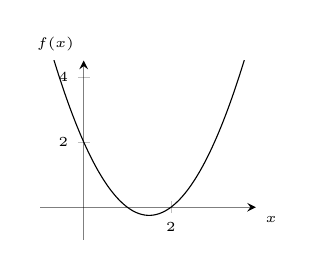
\begin{tikzpicture}
		\begin{axis}[scale=.4,draw opacity =.5,samples=100,smooth, 
		  axis x line=center, 
		  axis y line=center,
		  ylabel = {$f(x)$},
		  xlabel = {$x$},
		  xlabel style={below right},
		  ylabel style={above left},
		  xmin=-1,xmax=3.5,ymin=-1,ymax=4,
		  label style={font=\tiny},
		  tick label style={font=\tiny},
		  enlargelimits=upper] 
		  \addplot[black,opacity=1,domain=-2:5]{x^2-3*x+2};
		\end{axis}
	    \end{tikzpicture}
	    \end{center}
	    \vspace{.5cm}

	\end{enumerate}

    %-------------------- 2.
    \item $f(x)=x^3-4x$.\\\\
    	Respuesta.-\;

	\begin{enumerate}
	    \item Derivando $f(x)$, tenemos $f'(x)=3x^2-4$. Luego igualando a $0$,
		$$3x^2-4=0\quad \Rightarrow \quad x=\pm \dfrac{2}{\sqrt{3}}.$$
	    \item Por el teorema 4.7 (Tom Apostol, capítulo 4), podemos señalar que $f'$ es creciente si $|x|>\dfrac{2}{\sqrt{3}}$ y decreciente si $|x|<\dfrac{2}{\sqrt{3}}.$ 
	    \item Sea $f''(x)=6x$. Por lo tanto, $f'$ es creciente para $x>0$ y decreciente para $x<0$.
	    \item \;
	    \begin{center}
		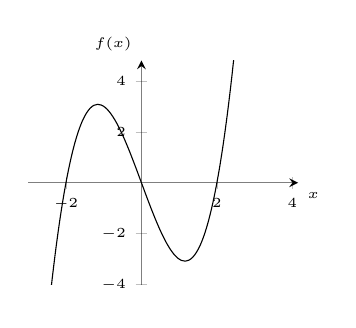
\begin{tikzpicture}
		\begin{axis}[scale=.5,draw opacity =.5,samples=100,smooth, 
		  axis x line=center, 
		  axis y line=center,
		  ylabel = {$f(x)$},
		  xlabel = {$x$},
		  xlabel style={below right},
		  ylabel style={above left},
		  xmin=-3,xmax=3.5,ymin=-4,ymax=4,
		  label style={font=\tiny},
		  tick label style={font=\tiny},
		  enlargelimits=upper] 
		  \addplot[black,opacity=1]{x^3-4*x};
		\end{axis}
	    \end{tikzpicture}
	    \end{center}
	    \vspace{.5cm}
	\end{enumerate}

    %-------------------- 3.
    \item $f(x)=(x-1)^2(x+2)$.\\\\
	Respuesta.-\;
	\begin{enumerate}
	\item Derivando $f(x)$, tenemos 
	    $$f'(x)=2(x-1)(x+2)+(x-1)^2=3(x^2-1)$$ 
	    Luego igualando a $0$,
		$$3(x^2-1)=0\quad \Rightarrow \quad x=\pm 1.$$
	    \item Por el teorema 4.7 (Tom Apostol, capítulo 4), podemos señalar que $f'$ es creciente si $|x|>1$ y decreciente si $|x|<-1.$ 
	    \item Sea $f''(x)=6x$. Por lo tanto, $f'$ es creciente para $x>0$ y decreciente para $x<0$.
	    \item \;
	    \begin{center}
		\begin{tikzpicture}
		\begin{axis}[scale=.5,draw opacity =.5,samples=100,smooth, 
		  axis x line=center, 
		  axis y line=center,
		  ylabel = {$f(x)$},
		  xlabel = {$x$},
		  xlabel style={below right},
		  ylabel style={above left},
		  xmin=-3,xmax=3.5,ymin=-4,ymax=6,
		  label style={font=\tiny},
		  tick label style={font=\tiny},
		  enlargelimits=upper] 
		  \addplot[black,opacity=1]{((x-1)^2)*(x+2)};
		\end{axis}
	    \end{tikzpicture}
	    \end{center}
	    \vspace{.5cm}
	\end{enumerate}

    %-------------------- 4.
    \item $f(x)=x^3-6x^2+9x+5.$\\\\
	Respuesta.-\;
	\begin{enumerate}
	\item Derivando $f(x)$, tenemos 
	    $$f'(x)=3x^2-12x+9.$$
	    Luego igualando a $0$,
		$$3(x^2-4x+3)=0\quad \Rightarrow \quad x_1=1,\quad x_2=3.$$
	    \item Por el teorema 4.7 (Tom Apostol, capítulo 4), podemos señalar que:
		$$\begin{array}{ccclcl}
		    \mbox{Si } &x<1 &\Rightarrow& f'(x)>0 &\Rightarrow& f\mbox{ es creciente.}\\
		    \mbox{Si } &1<x<3 &\Rightarrow& f'(x)<0 &\Rightarrow& f\mbox{ es decreciente.}\\
		    \mbox{Si } &x>3 &\Rightarrow& f'(x)>0 &\Rightarrow& f\mbox{ es creciente.}\\
		\end{array}$$
	    \item Sea $f''(x)=2x-4$. Entonces,
		$$2x-4>0 \; \Rightarrow \; x>2 \qquad \mbox{y} \qquad 2x-4<0 \; \Rightarrow \;x<2.$$
		Por lo tanto por el mismo criterio del teorema 4.7 (Tom Apostol, capítulo 4), se tiene que $f'$ es creciente si $x>2$ y decreciente si $x<2$.
	    \item \;
	    \begin{center}
		\begin{tikzpicture}
		\begin{axis}[scale=.5,draw opacity =.5,samples=100,smooth, 
		  axis x line=center, 
		  axis y line=center,
		  ylabel = {$f(x)$},
		  xlabel = {$x$},
		  xlabel style={below right},
		  ylabel style={above left},
		  xmin=-3,xmax=5,ymin=-5,ymax=15,
		  label style={font=\tiny},
		  tick label style={font=\tiny},
		  enlargelimits=upper] 
		  \addplot[black,opacity=1]{x^3-6*x^2+9*x+5};
		\end{axis}
	    \end{tikzpicture}
	    \end{center}
	    \vspace{.5cm}
	\end{enumerate}

    %-------------------- 5.
    \item $f(x)=2+(x-1)^4$.\\\\
	Respuesta.-\;
	\begin{enumerate}
	\item Derivando $f(x)$, tenemos 
	    $$f'(x)=4(x-1)^3.$$
	    Luego igualando a $0$,
		$$(x-1)^3=0\quad \Rightarrow \quad x=1.$$
	    \item Por el teorema 4.7 (Tom Apostol, capítulo 4), podemos señalar que:
		$$\begin{array}{ccclcl}
		    \mbox{Si } &x<1 &\Rightarrow& f'(x)<0 &\Rightarrow& f\mbox{ es decreciente.}\\
		    \mbox{Si } &x>1 &\Rightarrow& f'(x)>0 &\Rightarrow& f\mbox{ es creciente.}\\
		\end{array}$$
	    \item Sea $f''(x)=12(x-1)^2$. Ya que $(x-1)^2>0$. Por lo tanto por el mismo criterio del teorema 4.7 (Tom Apostol, capítulo 4), se tiene que $f'$ es creciente para todo $x$.
	    \item \;
	    \begin{center}
		\begin{tikzpicture}
		\begin{axis}[scale=.5,draw opacity =.5,samples=100,smooth, 
		  axis x line=center, 
		  axis y line=center,
		  ylabel = {$f(x)$},
		  xlabel = {$x$},
		  xlabel style={below right},
		  ylabel style={above left},
		  xmin=-2,xmax=4,ymin=-5,ymax=15,
		  label style={font=\tiny},
		  tick label style={font=\tiny},
		  enlargelimits=upper] 
		  \addplot[black,opacity=1]{2+(x-1)^4};
		\end{axis}
	    \end{tikzpicture}
	    \end{center}
	    \vspace{.5cm}
	\end{enumerate}

    %-------------------- 6.
    \item $f(x)=\dfrac{1}{x^2}.$\\\\
	Respuesta.-\;
	\begin{enumerate}
	\item Derivando $f(x)$, tenemos 
	    $$f'(x)=-\dfrac{2x}{x^4}=\dfrac{2}{x^3}.$$
	    Luego igualando a $0$,
	    $$-\dfrac{2}{x^3}=0\quad \Rightarrow \quad f'(x) \mbox{ es nunca cero}.$$
	    \item Por el teorema 4.7 (Tom Apostol, capítulo 4), podemos señalar que:
		$$\begin{array}{ccclcl}
		    \mbox{Si } &x<0 &\Rightarrow& f'(x)<0 &\Rightarrow& f\mbox{ es decreciente.}\\
		    \mbox{Si } &x>0 &\Rightarrow& f'(x)>0 &\Rightarrow& f\mbox{ es creciente.}\\
		\end{array}$$
	    \item Sea $f''(x)=\dfrac{6}{x^4}$. Por lo tanto $f'$ es decreciente para todo $x\neq 0$ y $x=0$ no está definido.
	    \item \;
	    \begin{center}
		\begin{tikzpicture}
		\begin{axis}[scale=.5,draw opacity =.5,samples=100,smooth, 
		  axis x line=center, 
		  axis y line=center,
		  ylabel = {$f(x)$},
		  xlabel = {$x$},
		  xlabel style={below right},
		  ylabel style={above left},
		  xmin=-3,xmax=3,ymin=-2,ymax=10.5,
		  label style={font=\tiny},
		  tick label style={font=\tiny},
		  enlargelimits=upper] 
		  \addplot[black,opacity=1]{1/(x^2)};
		\end{axis}
	    \end{tikzpicture}
	    \end{center}
	    \vspace{.5cm}
	\end{enumerate}

    %-------------------- 7.
    \item $f(x)=x+\dfrac{1}{x^2}.$\\\\
	Respuesta.-\;
	\begin{enumerate}
	\item Derivando $f(x)$, tenemos 
	    $$f'(x)=1+\dfrac{2}{x^3}.$$
	    Luego igualando a $0$,
	    $$1+\dfrac{2}{x^3}=0\quad \Rightarrow \quad x=\sqrt[3]{2}.$$
	    \item Por el teorema 4.7 (Tom Apostol, capítulo 4), podemos señalar que:
		$$\begin{array}{ccclcl}
		    \mbox{Si } &x<0 &\Rightarrow& f'(x)>0 &\Rightarrow& f\mbox{ es creciente.}\\
		    \mbox{Si } &1<x<\sqrt[3]{2} &\Rightarrow& f'(x)<0 &\Rightarrow& f\mbox{ es decreciente.}\\
		    \mbox{Si } &x>\sqrt[3]{2} &\Rightarrow& f'(x)>0 &\Rightarrow& f\mbox{ es creciente.}\\
		\end{array}$$
	    \item Sea $f''(x)=\dfrac{6}{x^4}$. Entonces, $f'$ es creciente para todo $x\neq 0$ y $x=0$ no está definido.
	    \item \;
	    \begin{center}
		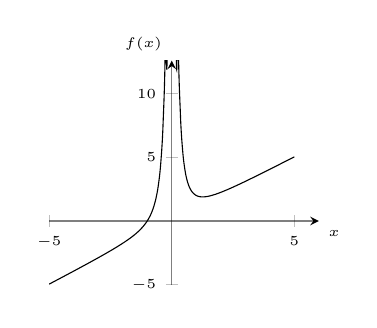
\begin{tikzpicture}
		\begin{axis}[scale=.5,draw opacity =.5,samples=100,smooth, 
		  axis x line=center, 
		  axis y line=center,
		  ylabel = {$f(x)$},
		  xlabel = {$x$},
		  xlabel style={below right},
		  ylabel style={above left},
		  xmin=-5,xmax=5,ymin=-5,ymax=11,
		  label style={font=\tiny},
		  tick label style={font=\tiny},
		  enlargelimits=upper] 
		  \addplot[black,opacity=1]{x+(1/x^2)};
		\end{axis}
	    \end{tikzpicture}
	    \end{center}
	    \vspace{.5cm}
	\end{enumerate}

    %-------------------- 8.
    \item $f(x)=\dfrac{1}{(x-1)(x-3)}$.\\\\
	Respuesta.-\;
	\begin{enumerate}
	\item Derivando $f(x)$, tenemos 
	    $$f'(x)=-\dfrac{2x-4}{(x-1)^2(x-3)^2}.$$
	    Luego igualando a $0$,
	    $$-\dfrac{2x-4}{(x-1)^2(x-3)^2}=0\quad \Rightarrow \quad x=2.$$
	    \item Por el teorema 4.7 (Tom Apostol, capítulo 4), y teniendo en cuenta que la función no está definida en $x=1$ y $x=3$, podemos señalar que:
		$$\begin{array}{ccclcl}
		    \mbox{Si } &x<1 &\Rightarrow& f'(x)>0 &\Rightarrow& f\mbox{ es creciente.}\\
		    \mbox{Si } &1<x<2 &\Rightarrow& f'(x)>0 &\Rightarrow& f\mbox{ es creciente.}\\
		    \mbox{Si } &2<x<3 &\Rightarrow& f'(x)<0 &\Rightarrow& f\mbox{ es decreciente.}\\
		    \mbox{Si } &x>3 &\Rightarrow& f'(x)<0 &\Rightarrow& f\mbox{ es decreciente.}\\
		\end{array}$$
	    \item Sea $f''(x)=\dfrac{1}{(x-3)^3}-\dfrac{1}{(x-1)^3}$. Entonces, $f'$ es creciente para todo $x\neq 1$ y $x>3$ y $f'$ es decreciente para $1<x<3$.\\\\
	    \item \;
	    \begin{center}
		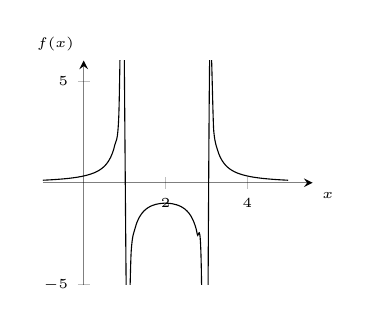
\begin{tikzpicture}
		\begin{axis}[scale=.5,draw opacity =.5,samples=100,smooth, 
		  axis x line=center, 
		  axis y line=center,
		  ylabel = {$f(x)$},
		  xlabel = {$x$},
		  xlabel style={below right},
		  ylabel style={above left},
		  xmin=-1,xmax=5,ymin=-5,ymax=5,
		  label style={font=\tiny},
		  tick label style={font=\tiny},
		  enlargelimits=upper] 
		  \addplot[black,opacity=1]{(1)/((x-1)*(x-3))};
		\end{axis}
	    \end{tikzpicture}
	    \end{center}
	    \vspace{.5cm}
	\end{enumerate}

    %-------------------- 9.
    \item $f(x)=\dfrac{x}{1+x^2}$.\\\\
	Respuesta.-\;
	\begin{enumerate}
	\item Derivando $f(x)$, tenemos 
	    $$f'(x)=\dfrac{1-x^2}{(1+x^2)^2}$$
	    Luego igualando a $0$,
	    $$\dfrac{1-x^2}{(1+x^2)^2}=0\quad \Rightarrow \quad x=\pm 1.$$
	    \item Por el teorema 4.7 (Tom Apostol, capítulo 4), podemos señalar que:
		$$\begin{array}{ccclcl}
		    \mbox{Si } &|x|<1 &\Rightarrow& f'(x)>0 &\Rightarrow& f\mbox{ es creciente.}\\
		    \mbox{Si } &|x|>1 &\Rightarrow& f'(x)<0 &\Rightarrow& f\mbox{ es decreciente.}\\
		\end{array}$$
	    \item Sea $f''(x)=\dfrac{2x(x^2-3)}{(1+x^2)^3}$. Entonces, $f'$ es creciente para todo $-\sqrt{3}<x<0$ o $x>\sqrt{3}$ y $f'$ es decreciente para $x<-\sqrt{3}$ o $0<x<\sqrt{3}.$
	    \item \;
	    \begin{center}
		\begin{tikzpicture}
		\begin{axis}[scale=.5,draw opacity =.5,samples=100,smooth, 
		  axis x line=center, 
		  axis y line=center,
		  ylabel = {$f(x)$},
		  xlabel = {$x$},
		  xlabel style={below right},
		  ylabel style={above left},
		  xmin=-5,xmax=5,ymin=-.8,ymax=.8,
		  label style={font=\tiny},
		  tick label style={font=\tiny},
		  enlargelimits=upper] 
		  \addplot[black,opacity=1]{(x)/(1+x^2)};
		\end{axis}
	    \end{tikzpicture}
	    \end{center}
	    \vspace{.5cm}
	\end{enumerate}

    %-------------------- 10.
    \item $f(x)=\dfrac{x^2-4}{x^2-9}$.\\\\
	Respuesta.-\;
	\begin{enumerate}
	    \item Derivando $f(x)$, tenemos 
	    $$f'(x)=-\dfrac{10x}{(x^2-9)^2}$$
	    Luego igualando a $0$,
	    $$-\dfrac{10x}{(x^2-9)^2}=0\quad \Rightarrow \quad x=0.$$
	    \item Por el teorema 4.7 (Tom Apostol, capítulo 4), podemos señalar que:
		$$\begin{array}{ccclcl}
		    \mbox{Si } &x<-3 &\Rightarrow& f'(x)>0 &\Rightarrow& f\mbox{ es creciente.}\\
		    \mbox{Si } &-3<x<0 &\Rightarrow& f'(x)>0 &\Rightarrow& f\mbox{ es creciente.}\\
		    \mbox{Si } &0<x<3 &\Rightarrow& f'(x)<0 &\Rightarrow& f\mbox{ es decreciente.}\\
		    \mbox{Si } &x>3 &\Rightarrow& f'(x)<0 &\Rightarrow& f\mbox{ es decreciente.}\\
		\end{array}$$
	    \item Sea $f''(x)=\dfrac{30(x^2+3)}{(x^2-9)^3}$. Entonces, $f'$ es creciente para $x<-3$ o $x>3$ y $f'$ es decreciente para $-3<x<3$.
	    \item \;
	    \begin{center}
		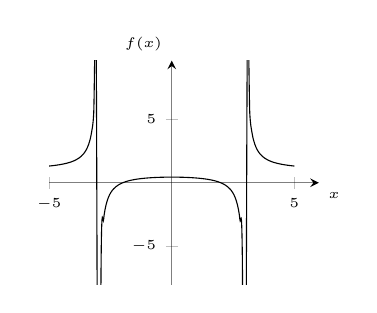
\begin{tikzpicture}
		\begin{axis}[scale=.5,draw opacity =.5,samples=100,smooth, 
		  axis x line=center, 
		  axis y line=center,
		  ylabel = {$f(x)$},
		  xlabel = {$x$},
		  xlabel style={below right},
		  ylabel style={above left},
		  xmin=-5,xmax=5,ymin=-8,ymax=8,
		  label style={font=\tiny},
		  tick label style={font=\tiny},
		  enlargelimits=upper] 
		  \addplot[black,opacity=1]{(x^2-4)/(x^2-9)};
		\end{axis}
	    \end{tikzpicture}
	    \end{center}
	    \vspace{.5cm}
	\end{enumerate}

    %-------------------- 11.
    \item $f(x)=\sen^2 x$.\\\\
	Respuesta.-\;
	\begin{enumerate}
	    \item Derivando $f(x)$, tenemos 
	    $$f'(x)=2\sen x \cdot \cos x=\sen(2x).$$
	    Luego igualando a $0$,
	    $$\sen(2x)=0\quad \Rightarrow \quad x=\dfrac{n\pi}{2}\qquad \mbox{para } n \mbox{ entero.}$$
	    \item $f$ es creciente si $n\pi < x < \left(n+\dfrac{1}{2}\right)\pi$ y decreciente si $\left(n-\dfrac{1}{2}\right)\pi<x<n\pi$
	    \item Sea $f''(x)=-2\cos(2x)$. Entonces, $f'$ es creciente si $\left(n-\dfrac{1}{4}\right)<x<\left(n+\dfrac{1}{4}\right)\pi$ y $f'$ es decreciente si  $\left(n+\dfrac{1}{4}\right)\pi<x<\left(n+\dfrac{3}{4}\right)\pi$.\\\\
	    \item \;
	    \begin{center}
		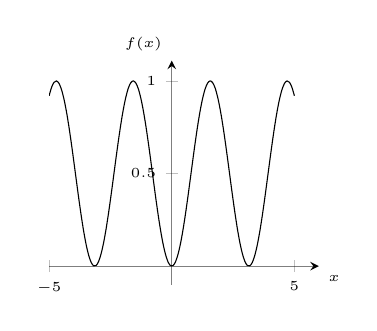
\begin{tikzpicture}
		\begin{axis}[scale=.5,draw opacity =.5,samples=100,smooth, 
		  axis x line=center, 
		  axis y line=center,
		  ylabel = {$f(x)$},
		  xlabel = {$x$},
		  xlabel style={below right},
		  ylabel style={above left},
		  xmin=-5,xmax=5,ymin=-.1,ymax=1,
		  label style={font=\tiny},
		  tick label style={font=\tiny},
		  enlargelimits=upper] 
		  \addplot[black,opacity=1]{(sin(deg(x)))^2};
		\end{axis}
	    \end{tikzpicture}
	    \end{center}
	    \vspace{.5cm}
	\end{enumerate}

    %-------------------- 12.
    \item $f(x)=x-\sen x$.\\\\
	Respuesta.-\;
	\begin{enumerate}
	    \item Derivando $f(x)$, tenemos 
	    $$f'(x)=1-\cos x.$$
	    Luego igualando a $0$,
	    $$1-\cos x=0\quad \Rightarrow \quad x=2n\pi.$$
	    \item $f$ es creciente para todo $x$ ya que $1-\cos x\geq 0$ para todo $x$.
	    \item Sea $f''(x)=\sen x$. Entonces, $f'$ es creciente si $2n\pi < x < (2+1)\pi$ y $f'$ es decreciente si $(2n-1)\pi<x<2n\pi.$ 
	    \item \;
	    \begin{center}
		\begin{tikzpicture}
		\begin{axis}[scale=.5,draw opacity =.5,samples=100,smooth, 
		  axis x line=center, 
		  axis y line=center,
		  ylabel = {$f(x)$},
		  xlabel = {$x$},
		  xlabel style={below right},
		  ylabel style={above left},
		  xmin=-5,xmax=5,ymin=-5,ymax=5,
		  label style={font=\tiny},
		  tick label style={font=\tiny},
		  enlargelimits=upper] 
		  \addplot[black,opacity=1]{x-sin(deg(x))};
		\end{axis}
	    \end{tikzpicture}
	    \end{center}
	    \vspace{.5cm}
	\end{enumerate}

    %-------------------- 13.
    \item $f(x)=x+\cos x$.\\\\
	Respuesta.-\;
	\begin{enumerate}
	    \item Derivando $f(x)$, tenemos 
		$$f'(x)=1-\sen x$$
	    Luego igualando a $0$,
	    $$1-\sen x=0\quad \Rightarrow \quad x=\left(2n+\dfrac{1}{2}\right)\pi.$$
	\item $f$ es creciente para todo $x$, ya que $1-\sen x \geq 0$ para todo $x$.
	    \item Sea $f''(x)=-\cos x$. Entonces, $f'$ es creciente si $\left(2n-\dfrac{1}{2}\right)<x<\left(2n+\dfrac{3}{2}\right)\pi$ y $f'$ es decreciente si  $\left(2-\dfrac{1}{2}\right)\pi<x<\left(2n+\dfrac{1}{2}\right)\pi$.\\\\
	    \item \;
	    \begin{center}
		\begin{tikzpicture}
		\begin{axis}[scale=.5,draw opacity =.5,samples=100,smooth, 
		  axis x line=center, 
		  axis y line=center,
		  ylabel = {$f(x)$},
		  xlabel = {$x$},
		  xlabel style={below right},
		  ylabel style={above left},
		  xmin=-5,xmax=5,ymin=-5,ymax=5,
		  label style={font=\tiny},
		  tick label style={font=\tiny},
		  enlargelimits=upper] 
		  \addplot[black,opacity=1]{x+cos(deg(x))};
		\end{axis}
	    \end{tikzpicture}
	    \end{center}
	    \vspace{.5cm}
	\end{enumerate}

    %-------------------- 14.
    \item $f(x)=\dfrac{1}{6}x^2+\dfrac{1}{12}\cos 2x$.\\\\
	Respuesta.-\;
	\begin{enumerate}
	    \item Derivando $f(x)$, tenemos 
		$$f'(x)=\dfrac{1}{3}x-\dfrac{1}{6}\sen(2x).$$
	    Luego igualando a $0$,
	    $$\dfrac{1}{3}x-\dfrac{1}{6}\sen(2x)=0\quad \Rightarrow \quad x=0.$$
	    \item $f$ es creciente si $x>0$ y decreciente si $x<0.$
	    \item Sea $f''(x)=\dfrac{1}{3}-\dfrac{1}{2}\cos(2x)$. Entonces, $f'$ es creciente para todo $x$.
	    \item \;
	    \begin{center}
		\begin{tikzpicture}
		\begin{axis}[scale=.5,draw opacity =.5,samples=100,smooth, 
		  axis x line=center, 
		  axis y line=center,
		  ylabel = {$f(x)$},
		  xlabel = {$x$},
		  xlabel style={below right},
		  ylabel style={above left},
		  xmin=-4,xmax=4,ymin=-.1,ymax=2,
		  label style={font=\tiny},
		  tick label style={font=\tiny},
		  enlargelimits=upper] 
		  \addplot[black,opacity=1]{1/6*x^2+1/12*cos(2*deg(x))};
		\end{axis}
	    \end{tikzpicture}
	    \end{center}
	    \vspace{.5cm}
	\end{enumerate}

\end{enumerate}


\end{comment}

\section{Ejemplos resueltos de problemas de extremos}

\begin{ejem}[Principio del producto máximo con suma constante]
    Dado un número positivo $S$. Demostrar que entre todos los pares de números positivos $x$ e $y$ tales que $x+y=S$, el producto $xy$ es el mayor cuando $x=y=\dfrac{1}{2}S.$\\\\
	Demostración.-\; Si $x+y=S,$ $y=S-x$ y el producto $xy$ es igual a $x(S-x)=xS-x^2$. Pongamos $f(x)=xS-x^2$. Este polinomio cuadrático tiene como deriva primera $f'(x)=S-2x$ que es positiva para $x<\frac{1}{2}S$ y negativa para $x>\dfrac{1}{2}S$. Por tanto el máximo de $xy$ se presenta cuando $x=\dfrac{1}{2}S$, $y=S-x=\dfrac{1}{2}S$. Esto también se puede demostrar sin utilizar el Cálculo. Pongamos simplemente $f(x)=\dfrac{1}{4}-\left(x-\dfrac{1}{2}S\right)^2$ y observamos que $f(x)$ es máximo cuando $x=\dfrac{1}{2}S$.\\
\end{ejem}

\begin{ejem}[Principio de suma mínima, con producto constante]
    Dado un número positivo $P$. Demostrar que entre todos los pares de números positivos $x$ e $y$ tales que $xy=P$, el que hace la suma $x+y$ mínima es $x=y=\sqrt{P}.$\\\\
    Demostración.-\; Tenemos que determinar el mínimo de la función $f(x)=x+\dfrac{P}{x}$ para $x>0$. La primera derivada es $f'(x)=1-\dfrac{P}{x^2}$. Esta es negativa para $x^2<P$ y positiva para $x^2>P$, de manera que $f(x)$ tiene su mínimo en $x=\sqrt{P}$. Luego, la suma $x+y$ es mínima cuando $x=y=\sqrt{P}.$\\\\
\end{ejem}

\begin{ejem}
    Entre los rectángulos de perímetro dado, el cuadrado es el de mayor área.\\\\
	Demostración.-\; Utilizando el resultado del ejemplo 4.1 Tom Apostol. Sea $x$ e $y$ los lados de un rectángulo cualquiera. Si el perímetro está fijado, entonces $x+y$ es constante, con lo que el área $xy$ tiene mayor valor cuando $x=y$. Luego, el rectángulo máximo es el cuadrado.\\\\
\end{ejem}

\begin{ejem}
    La media geométrica de dos números positivos no excede a su media aritmética. Esto es, $\sqrt{ab}\leq \frac{1}{2}(a+b).$\\\\
    Demostración.-\; Dados $a>0$, $b>0$, sea $P=ab$. Entre todos los positivos $x$ e $y$ siendo $xy=P$, la suma $x+y$ es la menor cuando $x=y=\sqrt{P}.$ Es decir, si $xy=P$ entonces $x+y\geq \sqrt{P}+\sqrt{P}=2\sqrt{P}.$ En particular, $a+b\geq 2\sqrt{P}=2\sqrt{ab}$, con lo que $\sqrt{ab}\leq \frac{1}{2}(a+b)$. La igualdad se presenta si y sólo si $a=b.$\\\\
\end{ejem}

\begin{ejem}
    Un bloque de peso $W$ es movido a lo largo de un plano por una fuerza que forma un ángulo $\theta$ con la recta de la dirección del movimiento, siendo $0\leq \theta \leq \frac{1}{2}\pi,$, como se ve en la figura 4.15 Tom Apostol. Supongamos que la resistencia por fricción es proporcional a la fuerza normal con la que el bloque presiona perpendicularmente contra el plano. Hallar el ángulo $\theta$ para el que la fuerza de propulsión necesaria para vencer la fricción sea lo más pequeña posible.\\\\
	Demostración.-\; 
\end{ejem}

\section{Ejercicios}

\begin{enumerate}[\bfseries 1.]

    %-------------------- 1.
    \item Demostrar que entre todos los rectángulos de área dada, el cuadrado es el de perímetro mínimo.\\\\
	Demostración.-\; Sea $x$ e $y$ denotado por los lados del rectángulo. Si el área es fija, entonces $xy$ es una constante, tal que $xy=A$. El perímetro de un rectángulo viene dado por $P(x,y)=2x+2y$, de donde
	$$P(x)=2x+2\dfrac{A}{x}.$$
	Para encontrar el valor mínimo, tomamos la derivada de $P(x)$,
	$$P'(x)=2-\dfrac{2A}{x^2}.$$
	Luego igualamos a cero y resolvemos para $x$,
	$$2-\dfrac{2A}{x^2}=0\quad \Rightarrow \quad x=\sqrt{A}.$$
	Ya que, $P'(x)<0$, cuando $x<\sqrt{A}$ y $P'(x)>0$, cuando $x>\sqrt{A}$ por el teorema 4.8 Apostol, se tiene que $f$ tiene un mínimo relativo en $\sqrt{A}.$. Como $x=\sqrt{A}$ implica $y=\sqrt{A}$, tenemos que el perímetro es mínimo cuando $x=y$. Es decir, cuando el rectángulo es un cuadrado.\\\\

    %-------------------- 2.
    \item Un granjero tiene $L$ pies de alambre para cercar un terreno de pasto rectangular adyacente a un muro de piedra. ¿Qué dimensiones darán el área máxima al terreno cercado?.\\\\
	Respuesta.-\; Sea $y$ el ancho de la pradera (es decir, la longitud de los lados perpendiculares a la pared) y sea $x$ la longitud de la pradera (es decir, la longitud del lado del rectángulo que es paralelo a la pared). Entonces, tenemos lo $2y + x = L$ que implica $x = L - 2$.  Entonces queremos maximizar
	$$A(y)=(L-2y)y=Ly-2y^2.$$
	Derivando se tiene,
	$$A'(y)=L-4y.$$
	Igualando a cero,
	$$L-4y=0\quad \Rightarrow \quad y=\dfrac{L}{4}y.$$ 
	Así, $A'(y)>0$ cuando $y<\dfrac{L}{4}$ y $A'(y)<0$ cuando $y>\dfrac{L}{4}$. Por el teorema 4.8 Apostol, $A(y)$ toma el valor máximo cuando $y=\dfrac{L}{4}.$ Luego,
	$$x=L-2y=L2\dfrac{L}{4}=\dfrac{L}{2}.$$
	De donde las dimensiones serán $\dfrac{L}{2}$ por $\dfrac{L}{4}.$\\\\

    %-------------------- 3.
    \item Un granjero quiere cercar un terreno de pasto rectangular de área $A$ adyacente a un muro de piedra. ¿Qué dimensiones exigen la mínima cantidad de alambre de cerca?.\\\\
	Respuesta.-\; Sea $x$ la longitud del lado paralelo al muro de piedra e $y$ la longitud de los lados perpendiculares al muro de piedra. Entonces, $A = xy$ fija, por lo que $y = \frac{A}{x}$. La función que queremos minimizar es $P = x + 2y = x + \frac{2A}{x}$. Luego, tomando la derivada que tenemos,
	$$P'(x)=1-\dfrac{2A}{x^2}.$$
	Igualando a cero,
	$$1-\dfrac{2A}{x^2}=0\quad \Rightarrow \quad x=\sqrt{2A}.$$
	Así, $P'(x)<0$ cuando $x<\sqrt{2A}$ y $P'(x)>0$ cuando $x>\sqrt{2A}$. Por el teorema 4.8 Apostol, $P(x)$ toma el valor mínimo cuando $x=\sqrt{2A}$. De donde,
	$$y=\dfrac{A}{x}\quad \rightarrow \quad y=\dfrac{A}{2\sqrt{2A}}=\dfrac{\sqrt{2A}}{2}.$$\\

    %-------------------- 4.
    \item Dado $S > O$. Probar que entre todos los números positivos $x$ e $y$ tales que $x + y = S$, la suma $x^2 + y^2$ es mínima cuando $x=y$.\\\\
	Demostración.-\;  Ya que $x+y=S$ que implica $y=S-x$. Entonces, la función que queremos minimizar es 
	$$f(x)=x^2+(S-x)^2.$$ 
	Luego, tomando la derivada se tiene,
	$$f'(x)=2x-2(S-x)=4x-2S.$$
	Igualando a cero,
	$$4x-2S=0\quad \Rightarrow \quad x=\dfrac{S}{2}.$$
	Así, $f'(x)<0$ cuando $x<\dfrac{S}{2}$ y $f'(x)>0$ cuando $x>\dfrac{S}{2}$. Por el teorema 4.8 Apostol, $f(x)$ toma el valor mínimo cuando $x=\dfrac{S}{2}$. De donde,
	$$y=S-x=S-\dfrac{S}{2}=\dfrac{S}{2}.$$
	Por lo tanto la suma es mínima, cuando 
	$$x=y.$$\\

    %-------------------- 5.
    \item Dado $R > 0$. Probar que entre todos los números positivos $x$ e $y$ tales que $x^2 + y^2 = R$, la suma $x + y$ es máxima cuando $x = y$.\\\\
	Demostración.-\; Por la ecuación $x^2+y^2=R$ se tiene,
	$$y=\sqrt{R-x^2}.$$
	Entonces, encontramos el máximo de la función de la siguiente manera,
	$$f(x)=x+\sqrt{R-x^2}\quad \Rightarrow \quad f'(x)=1-\dfrac{x}{\sqrt{R-x^2}}.$$
	Luego, igualamos a cero,
	$$\dfrac{x}{\sqrt{R-x^2}}=1\quad \Rightarrow \quad x=\sqrt{\dfrac{R}{2}}.$$
	Así, $f'(x)>0$ cuando $x<\sqrt{\dfrac{R}{2}}$ y $f'(x)<0$ cuando $x>\sqrt{\dfrac{R}{2}}$. Por el teorema 4.8 Apostol, $f(x)$ toma el valor máximo cuando $x=\sqrt{\dfrac{R}{2}}$. De donde,
	$$y=\sqrt{R-x^2}=\sqrt{R-\dfrac{R}{2}}=\sqrt{\dfrac{R}{2}}=x.$$
	Por lo tanto la suma $x+y$ es máxima, cuando $x=y$.\\\\

    %-------------------- 6.
    \item Cada lado de un cuadrado tiene una longitud $L$. Demostrar que entre todos los cuadrados inscritos en el cuadrado dado, el de área mínima tiene lados de longitud $\frac{1}{2}L\sqrt{2}$.\\\\
	Respuesta.-\; Sea un cuadrado con aristas de longitud $L$ de donde $x+y=L$. Vemos que $x$ e $y$ son longitudes de las dos secciones de $L$ creadas por el punto en el que la esquina del cuadrado inscrito se encuentra con el borde del cuadrado exterior. Sea $e$ la longitud de la arista del cuadrado inscrito. Entonces, $x+y=L$ implica $y=L-x$. Pongamos $f(x)=e^2$, por lo que 
	$$\mbox{Área}=f(x)=e^2=x^2+y^2=x^2+(L-x)^2=2x^2-2Lx+L^2.$$
	Sacando la derivada,
	$$f'(x)=4x-2L.$$
	Igualando a cero,
	$$4x-2L=0\quad \Rightarrow \quad x=\dfrac{L}{2}.$$
	Así, $f'(x)<0$ cuando $x<\dfrac{L}{2}$ y $f'(x)>0$ cuando $x>\dfrac{L}{2}$. Por el teorema 4.8 Apostol, $f(x)$ toma el valor mínimo cuando $x=\dfrac{L}{2}$. Usando nuestra ecuación para $y$, tenemos 
	$$y=L-x=L-\dfrac{L}{2}=\dfrac{L}{2}.$$
	Finalmente, resolviendo para la longitud de la arista $e$,
	$$e^2=\left(\dfrac{L}{2}\right)^2+\left(\dfrac{L}{2}\right)^2=\dfrac{L^2}{2} \quad \Rightarrow \quad e=\dfrac{L}{\sqrt{2}}=\dfrac{\sqrt{2}}{2}L.$$\\

    %-------------------- 7.
    \item Cada lado de un cuadrado tiene una longitud $L$. Hallar el tamaño del cuadrado de máxima área que puede circunscribirse al cuadrado dado.\\\\
	Respuesta.-\; Sea la longitud de la arista del cuadrado circunscrito. Después $e=x+y$. Además, si $L$ es la longitud de la arista del cuadrado dado, tenemos
	$$x^2+y^2=L^2\quad \Rightarrow \quad y=\sqrt{L^2-x^2}.$$
	Sea $f(x)=\mbox{Área}=(x+y)^2$, entonces
	$$\mbox{Área}=f(x)=(x+y)^2=\left(L^2+x^2\right)^2=x^2+2x\sqrt{L^2-x^2}+L^2-x^2=2x\sqrt{L^2-x^2}+L^2.$$
	Sacando la derivada,
	$$f'(x)=2\sqrt{L^2-x^2}-\dfrac{2x}{\sqrt{L^2-x^2}}=2\dfrac{L^2-x^2-x}{\sqrt{L^2-x^2}}.$$
	Igualando a cero,
	$$2\dfrac{L^2-x^2-x}{\sqrt{L^2-x^2}}=0\quad \Rightarrow \quad x=\dfrac{L}{\sqrt{2}}.$$
	Así, $f'(x)>0$ cuando $x<\dfrac{L}{\sqrt{2}}$ y $f'(x)<0$ cuando $x>\dfrac{L}{\sqrt{2}}$. Por el teorema 4.8 Apostol, $f(x)$ toma el valor máximo cuando $x=\dfrac{L}{\sqrt{2}}$. Usando nuestra ecuación para $y$, tenemos
	$$y=\sqrt{L^2-\dfrac{L^2}{2}}=\sqrt{\dfrac{L^2}{2}}=\dfrac{L}{\sqrt{2}}.$$
	Finalmente, dado que $e=x+y$ tenemos el área del cuadrado circunscrito dada por
	$$\mbox{Área}=e^2=(x+y)^2=\left(\dfrac{L}{\sqrt{2}}+\dfrac{L}{\sqrt{2}}\right)^2=\left(\dfrac{2L}{\sqrt{2}}\right)^2=2L^2.$$\\

    %-------------------- 8.
    \item Demostrar que entre todos los rectángulos que pueden inscribirse en un círculo dado, el cuadrado tiene el área máxima.\\\\
	Demostración.-\; Sean $x$ e $y$ que denotan las longitudes de los lados del rectángulo inscrito, y $r$ denota el radio del círculo. Entonces $x^2+y^2=4r^2$ que implica $y=\sqrt{4r^2-x^2}$. Sea $f(x)=x\cdot y$. Entonces, derivando se tiene,
	$$\mbox{Área}=f(x)=xy=x\sqrt{4r^2-x^2}\quad \Rightarrow \quad f(x)=\dfrac{4r^2-2x^2}{\sqrt{4r^2-x^2}}.$$
	Luego, Igualando a cero,
	$$\dfrac{4r^2-2x^2}{\sqrt{4r^2-x^2}}=0\quad \Rightarrow \quad x=\sqrt{2}r.$$
	Así, $f'(x)<0$ cuando $x<\sqrt{2}r$ y $f'(x)>0$ cuando $x>\sqrt{2}r$. Por el teorema 4.8 Apostol, $f(x)$ toma el valor máximo cuando $x=\sqrt{2}r$. Usando nuestra ecuación para $y$, tenemos
	$$y=\sqrt{4r^2-x^2}=\sqrt{4r^2-2r^2}=\sqrt{2r^2}=\sqrt{2}r.$$
	Finalmente, $x=y$ por lo que el rectángulo es un cuadrado.\\\\

    %-------------------- 9.
    \item Demostrar que entre todos los rectángulos de área dada, el cuadrado tiene el círculo circunscrito mínimo.\\\\
	Demostración.-\; Sean $x$ e $y$ los lados del rectángulo, $r$ el radio del circulo circunscrito y $A=xy$ el área del cuadrado. Entonces,
	$$A=xy\quad \Rightarrow \quad y=\dfrac{A}{x}.$$
	Además, dado que tenemos un triángulo rectángulo cuya hipotenusa es el diámetro del círculo (por lo tanto es $2r$) y cuyos catetos son los lados del cuadrado que tenemos,
	$$\begin{array}{rcl}
	    (2r)^2=x^2+y^2&\Rightarrow &r=\dfrac{1}{2}\sqrt{x^2+y^2}\\\\
			  &\Rightarrow&r=\dfrac{1}{2}\sqrt{x^2+\left(\dfrac{A}{x}\right)^2}\\\\
			  &\Rightarrow&r=\dfrac{\sqrt{x^4+A^2}}{2x}.\\\\
	\end{array}$$
	Luego queremos encontrar el valor mínimo de esta función (ya que esta función nos da el radio del círculo). Llamemos a la función $f(x)$ y tomemos su derivada de la siguiente manera, 
	$$f'(x)=\dfrac{(2x)\left(\dfrac{1}{2}\right)\left(4x^3\right)\left(x^4-A^2\right)^{-\frac{1}{2}}-\left(\sqrt{x^4+A^2}\right)(2)}{4x^2}=\dfrac{x^2}{\sqrt{x^4+A^2}}-\dfrac{\sqrt{x^4-A^2}}{2x^2}.$$
	Igualando a cero,
	$$\dfrac{x^2}{\sqrt{x^4+A^2}}-\dfrac{\sqrt{x^4-A^2}}{2x^2}=0\quad \Rightarrow \quad x^4=a^2\quad \Rightarrow \quad x_1=\sqrt{A},\quad x_2=\sqrt{A}.$$
	Luego el punto critico es un mínimo ya que, $f'(x)<0$ cuando $x<\sqrt{A}$ y $f'(x)>0$ cuando $x>\sqrt{A}$. Por lo tanto, el radio del círculo se minimiza cuando $x=y=\sqrt{A}$, por lo que el rectángulo es un cuadrado.\\\\

    %-------------------- 10.
    \item Dada una esfera de radio $R$. Hallar el radio $r$ y la altura $h$ del cilindro circular recto de mayor superficie lateral $2\pi rh$ que puede inscribirse en la esfera.\\\\
	Demostración.-\; Primero, sea $h$ una función de $r$. Luego sea, un triángulo rectángulo con hipotenusa de longitud $r$ y catetos de longitud $\frac{h}{2}$ (ya que el segundo cateto solo llega al centro de la esfera, no a la longitud total del cilindro). Por lo tanto,
	$$R^2=r^2+\dfrac{h^2}{4}\quad \Rightarrow \quad h=2\sqrt{R^2-r^2}.$$
	Entonces, sabemos que el área de la superficie lateral, , viene dada por la fórmula
	$$A=2 \pi rh = 2\pi r\sqrt{R^2-r^2}=4\pi r\sqrt{R^2-r^2}.$$
	Llamando a esta función $f(r)$ y diferenciando tenemos,
	$$f'(r)=4\pi \sqrt{R^2-r^2}+\dfrac{4\pi r}{\sqrt{R^2-r^2}}.$$
	Igualando a cero,
	$$4\pi \sqrt{R^2-r^2}+\dfrac{4\pi r}{\sqrt{R^2-r^2}}=0\quad \Rightarrow \quad 2r^2=R^2\quad \Rightarrow \quad r=\dfrac{R}{\sqrt{2}}.$$
	Luego, $f'(r)<0$ cuando $r<\dfrac{R}{\sqrt{2}}$ y $f'(r)>0$ cuando $r>\dfrac{R}{\sqrt{2}}$. Por el teorema 4.8 Tom Apostol, $f(r)$ toma el valor mínimo cuando $r=\dfrac{R}{\sqrt{2}}.$ Por lo tanto, el área de la superficie lateral es mínima cuando 
	$$r=\dfrac{h}{2}=\sqrt{R^2-\dfrac{R^2}{2}}=\dfrac{R}{\sqrt{2}}.$$\\

    %-------------------- 11.
    \item Entre todos los cilindros circulares rectos de área lateral dada, demostrar que la menor
	esfera circunscrita tiene el radio igual al radio del cilindro multiplicado por $\sqrt{2}.$\\\\
	Demostración.-\; El área de la superficie lateral $A=2\pi rh$ es constante y 
	$$R^2=r^2+\dfrac{h^2}{4}.$$
	Entonces, tenemos
	$$A=2\pi rh \quad \Rightarrow \quad h=\dfrac{A}{2\pi r}.$$
	Por lo tanto,
	$$R^2=r^2+\dfrac{h^2}{4}=r^2+\dfrac{A^2}{16\pi^2 r^2} \quad \Rightarrow \quad R=\sqrt{r^2+\dfrac{A^2}{16\pi^2r^2}}.$$
	Llamemos a esta función $f'(r)=0$. Luego tomando la derivada,
	$$f'(r)=\dfrac{1}{2}\left(r^2+\dfrac{A^2}{16\pi^2 r^2}\right)^{-\frac{1}{2}}\left(2r-\dfrac{2A^2}{16\pi^2 r^3}\right).$$
	Igualando a cero,
	$$\dfrac{1}{2}\left(r^2+\dfrac{A^2}{16\pi^2 r^2}\right)^{-\frac{1}{2}}\left(2r-\dfrac{2A^2}{16\pi^2 r^3}\right)=0\quad \Rightarrow \quad 2r=\dfrac{A^2}{8\pi^2r^3} \quad \Rightarrow \quad r^4=\dfrac{A^2}{16\pi^2}\quad \Rightarrow \quad r=\dfrac{1}{2}\sqrt{\dfrac{A}{\pi}}.$$
	Luego, $f'(r)<0$ cuando $r<\dfrac{1}{2}\sqrt{\dfrac{A}{\pi}}$ y $f'(r)>0$ cuando $r>\dfrac{1}{2}\sqrt{\dfrac{A}{\pi}}$. Por el teorema 4.8 Tom Apostol, $f(r)$ toma el valor mínimo cuando $r=\dfrac{1}{2}\sqrt{\dfrac{A}{\pi}}.$ Por lo tanto, el radio de la esfera circunscrita es mínimo cuando
	$$R=\sqrt{r^2+\dfrac{A^2}{16\pi^2r^2}}=\sqrt{\dfrac{2A}{2\pi}}=\sqrt{2}r.$$\\

    %-------------------- 12.
    \item Dado Un cono circular recto de radio R y altura H. Hallar el radio y la altura del cilindro circular recto de mayor área lateral que puede inscribirse en el cono.\\\\
	Respuesta.-\; El área de la superficie lateral del cilindro viene dada por $A = 2 \pi rh$, donde res el radio del cilindro y hes la altura del cilindro. Del diagrama encontramos una fórmula para $h$ en términos de las constantes $H$ y $R$, y el radio del cilindro $r$,
	$$h=-\dfrac{H}{R}r+H.$$
	Así, sea $f(r)$ el área de la superficie lateral tenemos
	$$A=f(r)=2\pi rh = 2\pi r\left(-\dfrac{H}{R}r+H\right)=2\pi rH-\dfrac{2\pi H}{R}r^2.$$
	Tomando la derivada con respecto a $r$ e igualando a cero,
	$$2\pi H - \dfrac{4\pi H}{R}r=0 \quad \Rightarrow \quad R-2r=0\quad \Rightarrow \quad r=\dfrac{R}{2}.$$
	Luego, $f'(r)>0$ cuando $r<\dfrac{R}{2}$ y $f'(r)<0$ cuando $r>\dfrac{R}{2}$. Por el teorema 4.8 Tom Apostol, $f(r)$ toma el valor máximo cuando $r=\dfrac{R}{2}$. Por lo tanto, el área de la superficie lateral es máxima cuando
	$$h=\dfrac{1}{2}H.$$\\

    %-------------------- 13.
    \item Hallar las dimensiones del cilindro circular recto de máximo volumen que puede inscribirse en un cono circular recto de radio R y altura H.\\\\
	Respuesta.-\; Tenemos la siguiente expresión para h,
	$$h=-\dfrac{H}{R}r+H.$$
	Entonces,
	$$V=\pi r^2 h = \pi r^2 \left(-\dfrac{H}{R}r+H\right)=\pi r^2-\dfrac{\pi H}{R}r^3.$$
	Derivando con respecto a $r$,
	$$\dfrac{dV}{dr}=2\pi Hr-\dfrac{3\pi H}{R}r^2.$$
	Igualando a cero,
	$$\begin{array}{rcl}
	    2\pi Hr-\dfrac{3\pi H}{R}r^2=0&\Rightarrow& 2\pi H - \dfrac{3\pi H}{R}r=0\\\\
					  &\Rightarrow& 1-\dfrac{3}{2R}r=0\\\\
					  &\Rightarrow& r=\dfrac{2}{3}R.
	\end{array}$$
	Luego, $f'(r)>0$ cuando $r<\dfrac{2}{3}R$ y $f'(r)<0$ cuando $r>\dfrac{2}{3}R$. Por el teorema 4.8 Tom Apostol, $f(r)$ toma el valor máximo cuando $r=\dfrac{2}{3}R$. Por lo tanto, el volumen es máximo cuando
	$$h=\dfrac{2}{3}H.$$\\

    %-------------------- 14.
    \item Dada una esfera de radio $R$. Calcular, en función de $R$, el radio $r$ y la altura $h$ del cono circular recto de mayor volumen que puede inscribirse en esa esfera.\\\\
	Respuesta.-\; Queremos maximizar el volumen del cono,
	$$V=\dfrac{1}{3}\pi r^2 h.$$
	Luego podemos encontrar la siguiente expresión para $h$ en términos de $R$ y $r$,
	$$h=R+\sqrt{R^2-r^2}.$$
	Por lo tanto, nuestra expresión para $V$ en términos de $r$ es
	$$V=\dfrac{1}{3}\pi r^2 R + \dfrac{1}{3}\pi r^2 \sqrt{R^2-r^2}.$$
	Derivando con respecto a $r$,
	$$\dfrac{dV}{dr}=\dfrac{2}{3}\pi r R + \dfrac{2}{3}\pi r \sqrt{R^2-r^2} - \dfrac{1}{3}\pi r^3 \left(\dfrac{1}{\sqrt{R^2-r^2}}\right)=\dfrac{2}{3}\pi r \left(R+\sqrt{R^2-r^2}\right)-\dfrac{\pi r^3}{3\sqrt{R^2-r^2}}.$$
	Igualando a cero,
	$$\begin{array}{rcl}
	    \dfrac{2}{3}\pi r \left(R+\sqrt{R^2-r^2}\right)-\dfrac{\pi r^3}{3\sqrt{R^2-r^2}}=0 &\Rightarrow& R+\sqrt{R^2-r^2}-\dfrac{r^2}{2\sqrt{R^2-r^2}}=0\\\\
											       &\Rightarrow& 9r^2=8r^2R^2\\\\
											       &\Rightarrow& r=\dfrac{2\sqrt{2}}{3}R.
	\end{array}$$
	Luego, $f'(r)>0$ cuando $r<\dfrac{2\sqrt{2}}{3}R$ y $f'(r)<0$ cuando $r>\dfrac{2\sqrt{2}}{3}R$. Por el teorema 4.8 Tom Apostol, $f(r)$ toma el valor máximo cuando $r=\dfrac{2\sqrt{2}}{3}R$. Por lo tanto, el volumen es máximo cuando
	$$h=R+\sqrt{R^2-\dfrac{8}{9}R^2}=\dfrac{4}{3}R.$$\\

    %-------------------- 15.
    \item Hallar el rectángulo de mayor área que puede inscribirse en un semicírculo, teniendo la base inferior en el diámetro.\\\\
	Respuesta.-\; Sean $r$ el radio del semicirculo, $x$ la mitad de la base del rectángulo e $y$ la altura del rectángulo. Queremos maximizar el área, $A=2xy$ tal que 
	$$y=\sqrt{r^2-x^2}.$$
	Luego,
	$$A=2x\left(\sqrt{r^2-x^2}\right).$$
	Derivando con respecto a $x$,
	$$f'(x)=\dfrac{dA}{dx}=2\sqrt{r^2-x^2}-\dfrac{2x^2}{\sqrt{r^2-x^2}}.$$
	Igualando a cero,
	$$\begin{array}{rcl}
	    2\sqrt{r^2-x^2}-\dfrac{2x^2}{\sqrt{r^2-x^2}}=0 &\Rightarrow& 2\sqrt{r^2-x^2}=2x^2\\\\
	    							      &\Rightarrow& 2r^2-4x^2=0\\\\
								      &\Rightarrow& x=\dfrac{r}{\sqrt{2}}.
	\end{array}$$

	Luego, $f'(x)>0$ cuando $x<\dfrac{r}{\sqrt{2}}$ y $f'(x)<0$ cuando $x>\dfrac{r}{\sqrt{2}}$. Por el teorema 4.8 Tom Apostol, $f(x)$ toma el valor máximo cuando $x=\dfrac{r}{\sqrt{2}}$. 
	Ya que $y=\sqrt{r^2-x^2}$, entonces 
	$$y=\sqrt{r^2-\left(\dfrac{r}{\sqrt{2}}\right)^2}=\dfrac{r}{\sqrt{2}}.$$
	Por lo tanto, la base del rectángulo tiene longitud $\dfrac{2r}{\sqrt{2}}$ y su altura tiene longitud $\dfrac{r}{\sqrt{2}}$.\\\\


    %-------------------- 16.
    \item Hallar el trapecio de mayor área que puede inscribirse en un semicírculo, teniendo la base inferior en el diámetro.\\\\
	Respuesta.-\; Sea rel radio del semicírculo, $b_1$ sea el borde inferior del trapezoide y $b_2$ el borde superior. Recordamos de la geometría que el área del trapezoide está dada por
	$$A=\dfrac{1}{2}(b_1+b_2)h.,$$
	donde $b_1$ y $b_2$ son las longitudes de las bases y $h$ es la altura del trapezoide. A continuación, queremos encontrar fórmulas para $b_1$ y $b_2$ en función al radio $r$. Como $b_1$ se encuentra en el diámetro del semicírculo, tenemos $b_1 = 2r$. La hipotenusa de cada uno de estos es $r$, y los catetos tienen longitudes $h$ y $\dfrac{b_2}{2}$. Por lo tanto, 
	$$\begin{array}{rcl}
	    r^2=h^2+\left(\dfrac{b_2}{2}\right)^2 & \Rightarrow & r^2=h^2+\dfrac{b_2^2}{4}\\\\
						  & \Rightarrow & b_2^2=4r^2-4h^2\\\\
						  & \Rightarrow & b_2=2\sqrt{r^2-h^2}.
	\end{array}$$
	Sustituyendo estos en la fórmula para el área de un trapezoide, obtenemos una expresión para el área del trapezoide en función de $r$ y $h$,
	$$A=\dfrac{1}{2}h(b_1+b_2)=hr+h\sqrt{r^2-h^2}.$$
	Derivando con respecto a $h$,
	$$f'(h)=\dfrac{dA}{dh}=r+\sqrt{r^2-h^2}-\dfrac{h^2}{\sqrt{r^2-h^2}}.$$
	Igualamos a cero para encontrar los puntos críticos,
	$$\begin{array}{rcl}
	    r+\sqrt{r^2-h^2}-\dfrac{h^2}{\sqrt{r^2-h^2}}=0 &\Rightarrow& r\sqrt{r^2-h^2}+r^2-h^2-h^2\\\\
	    						      &\Rightarrow& 4h^4=3r^2h^2\\\\
							      &\Rightarrow& h=\dfrac{\sqrt{3}}{2}r.
	\end{array}$$
	Luego, $f'(h)>0$ cuando $h<\dfrac{\sqrt{3}}{2}r$ y $f'(h)<0$ cuando $h>\dfrac{\sqrt{3}}{2}r$. Por el teorema 4.8 Tom Apostol, $f(h)$ toma el valor máximo cuando $h=\dfrac{\sqrt{3}}{2}r$. Finalmente, usamos este valor $h$ para resolver $b_2$ en función de $r$,
	$$b_2=2\sqrt{r^2-h^2}=2\sqrt{\dfrac{r^2}{4}}r.$$
	Como $b_1=2r$, entonces las longitudes de los bordes superiores e inferiores del trapezoide son:
	$$b_1=2r,\qquad b_2=r.$$\\

    %-------------------- 17.
    \item 

\end{enumerate}



